\documentclass[11pt]{beamer}
\usetheme{Luebeck}
\usepackage[utf8]{inputenc}
\usepackage[english]{babel}
\usepackage{amsmath}
\usepackage{siunitx}
\usepackage{amsfonts}
\usepackage{amssymb}
\usepackage{graphicx}
\usepackage{booktabs}
\usepackage{subcaption}
\author{Eugenia Spedicato, Lina Maria Ortiz Parra, Jonah Blank}
\title{Detector induced assymetry in CP violation measurements}
%\setbeamercovered{transparent}
%\setbeamertemplate{navigation symbols}{}
%\logo{}
%\institute{}
%\date{}
%\subject{}
\begin{document}

\begin{frame}
\titlepage
\end{frame}

%\begin{frame}
%\tableofcontents
%\end{frame}

\begin{frame}
\begin{LARGE}
Progress 04.12.19
\end{LARGE}
\end{frame}
\begin{frame}{Total Efficiencies}
\begin{table}
	\begin{tabular}{cS[table-format=2.4]S[table-format=2.4]S[table-format=2.4]S[table-format=2.4]S[table-format=2.4]}
		\toprule
		{Polarity} & {$\epsilon_{\pi} $} & {$\epsilon_{K} $} & {$ \epsilon_{\pi,s} $} & {$\epsilon_{D^0} $} & {$\epsilon_{D^*} $} \\
		\midrule
		$UP$ & 86.6106 & 84.6535 & 76.6145 & 73.3255 & 56.2636 \\
		$DOWN$ & 86.6086 & 84.6657 & 76.5371 & 73.332 & 56.2344 \\
		\bottomrule
	\end{tabular}
\end{table}
\end{frame}
\begin{frame}{$\pi$-efficiency}
\begin{figure}
\begin{subfigure}{0.45\textwidth}
\includegraphics[width=0.9\textwidth]{up_pdf/tot/h_pt_reco_Pi.pdf}
\end{subfigure}
\begin{subfigure}{0.45\textwidth}
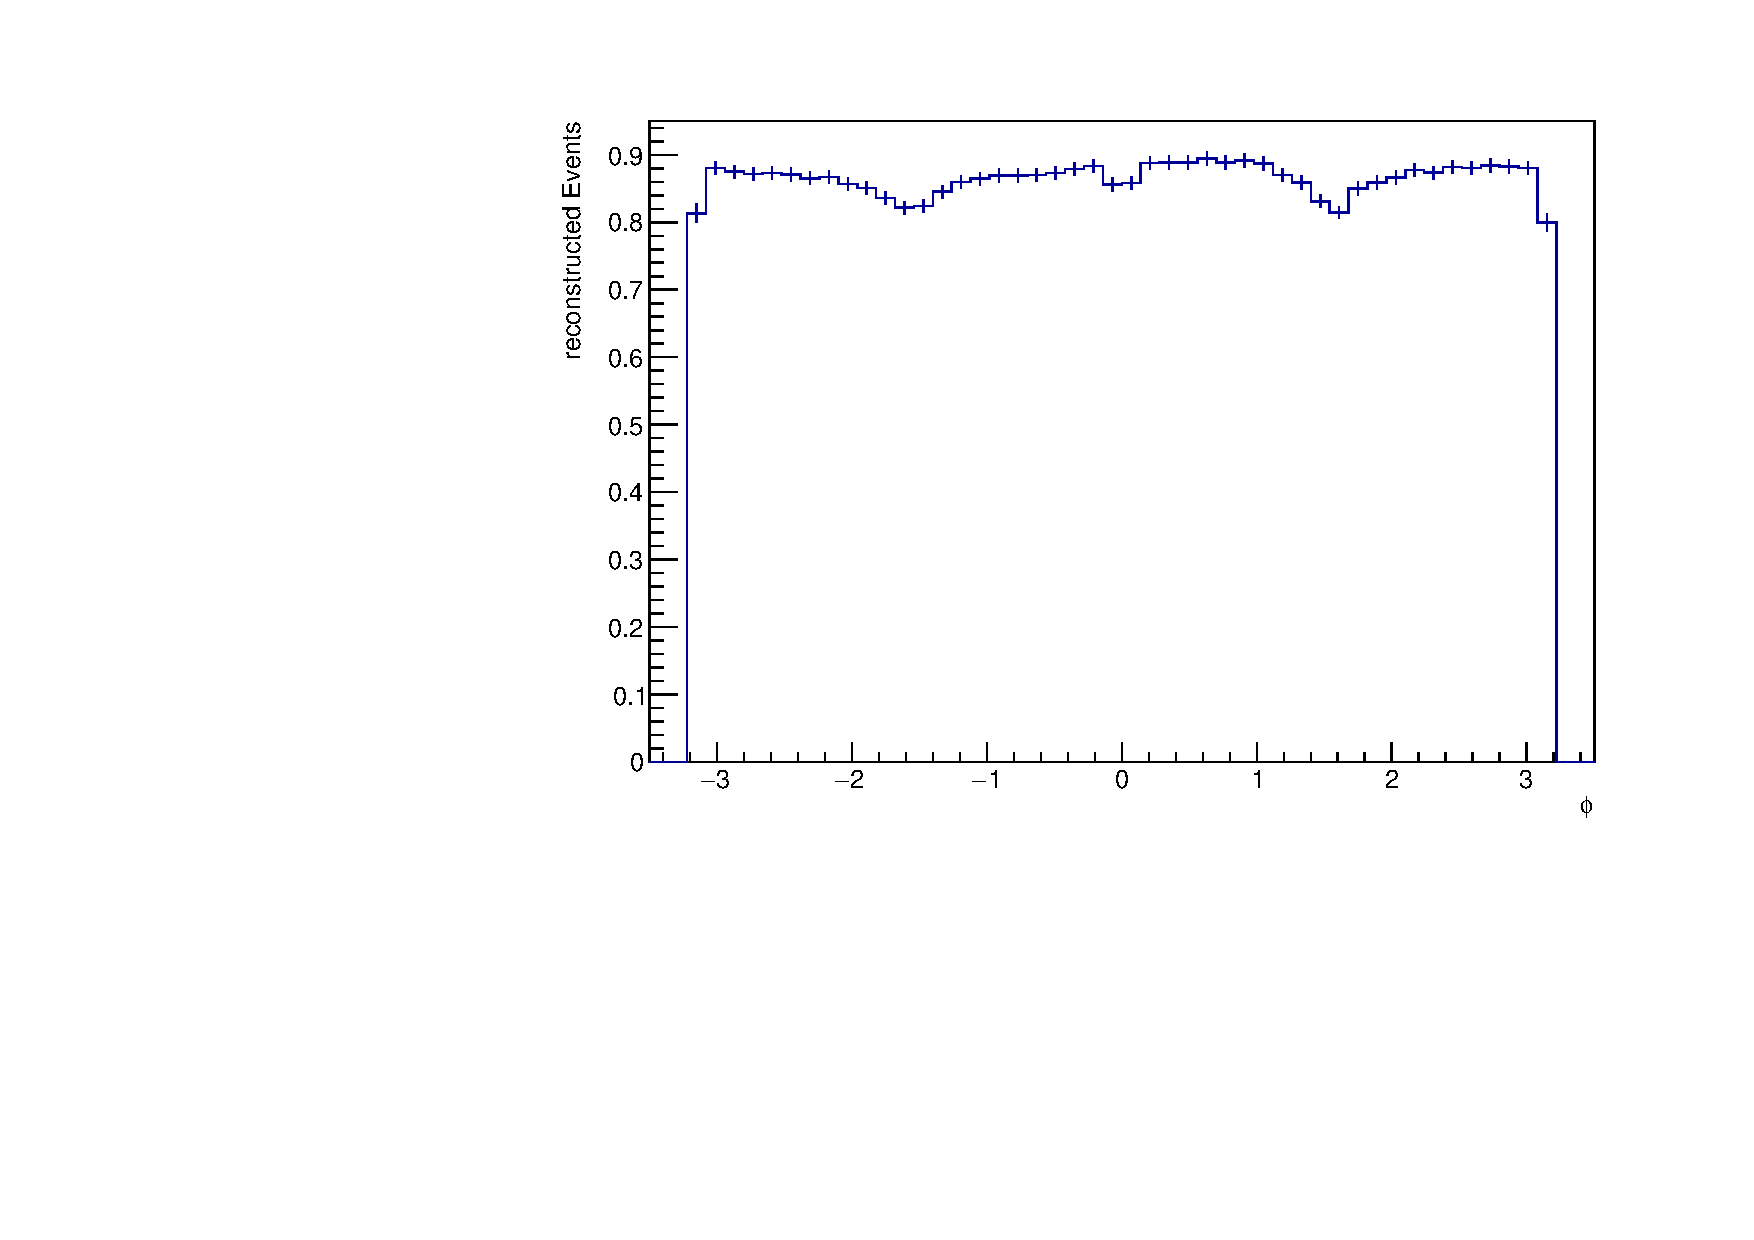
\includegraphics[width=0.9\textwidth]{up_pdf/tot/h_phi_reco_Pi.pdf}
\end{subfigure}
\begin{subfigure}{0.45\textwidth}
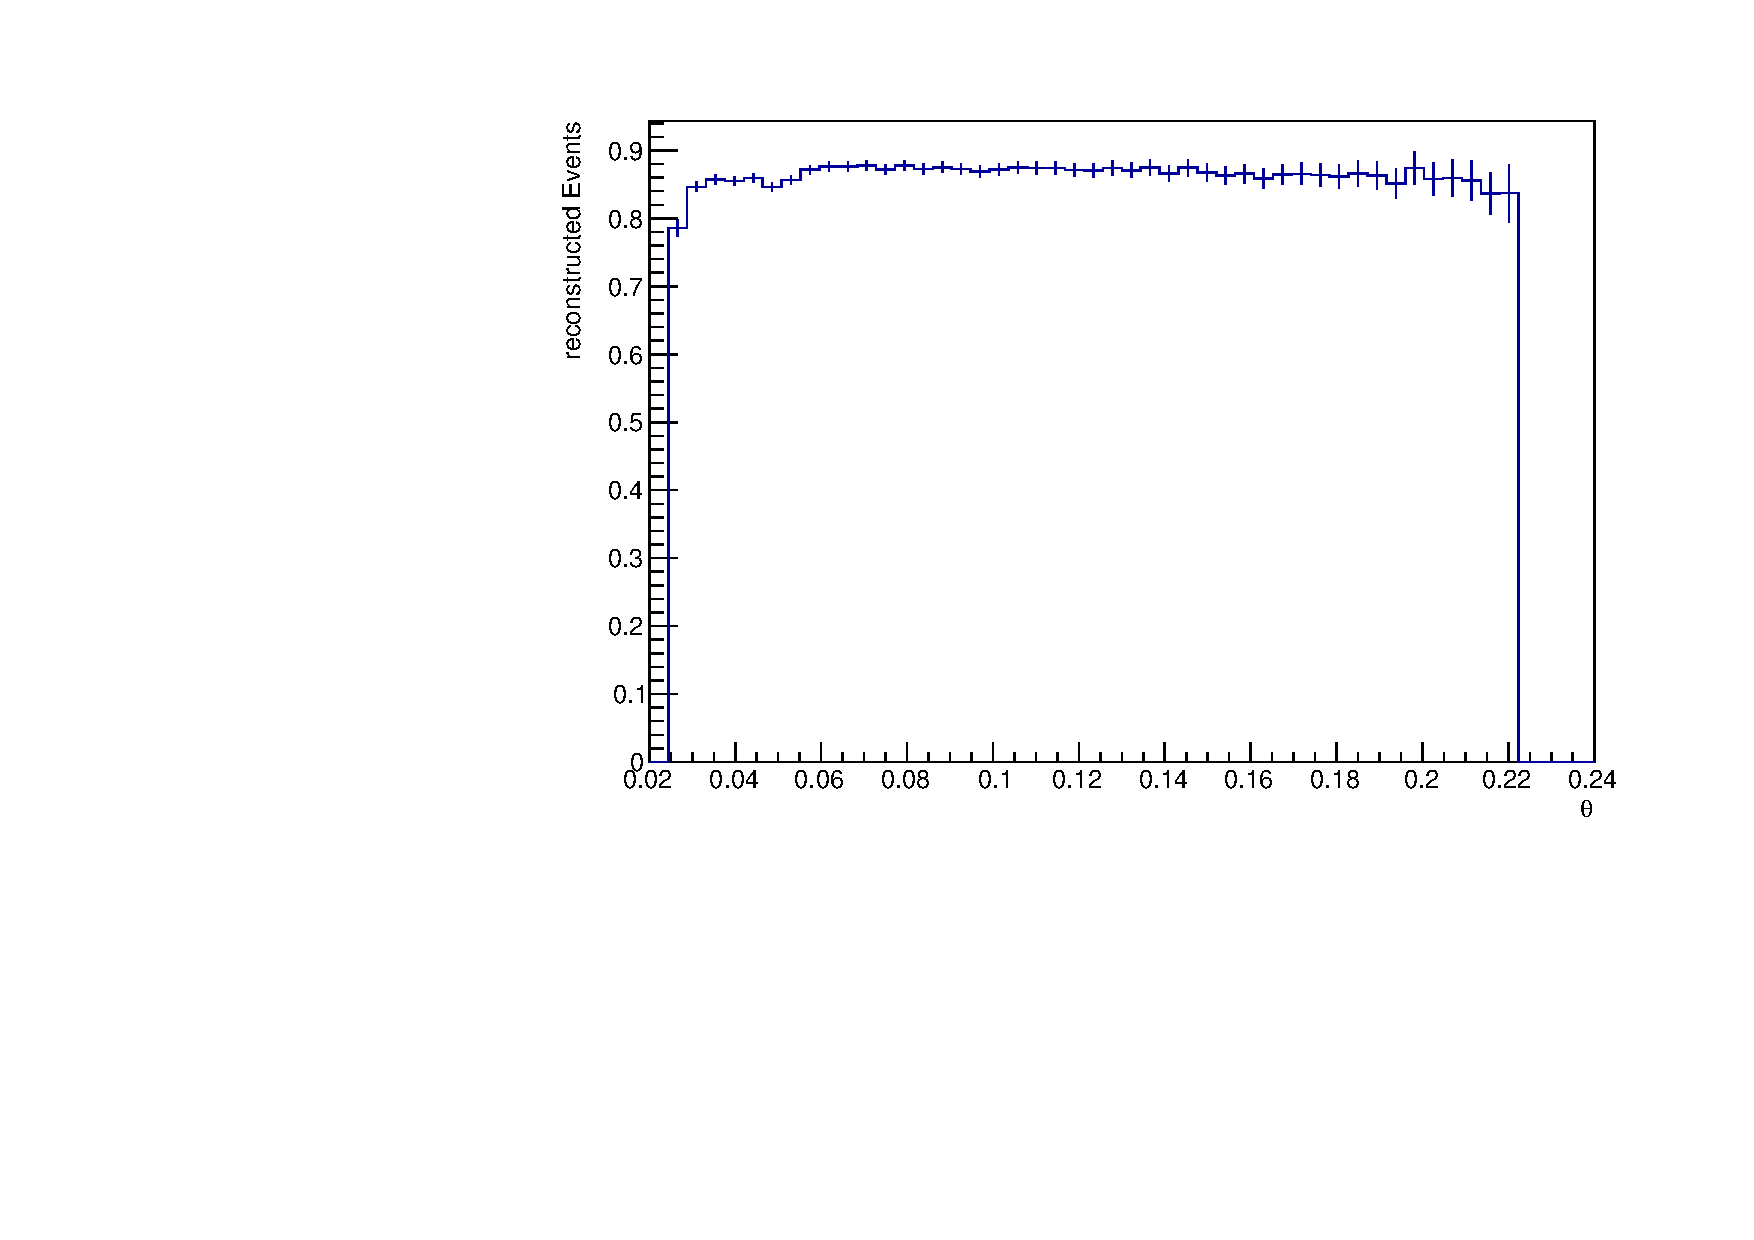
\includegraphics[width=0.9\textwidth]{up_pdf/tot/h_theta_reco_Pi.pdf}
\end{subfigure}
\begin{subfigure}{0.45\textwidth}
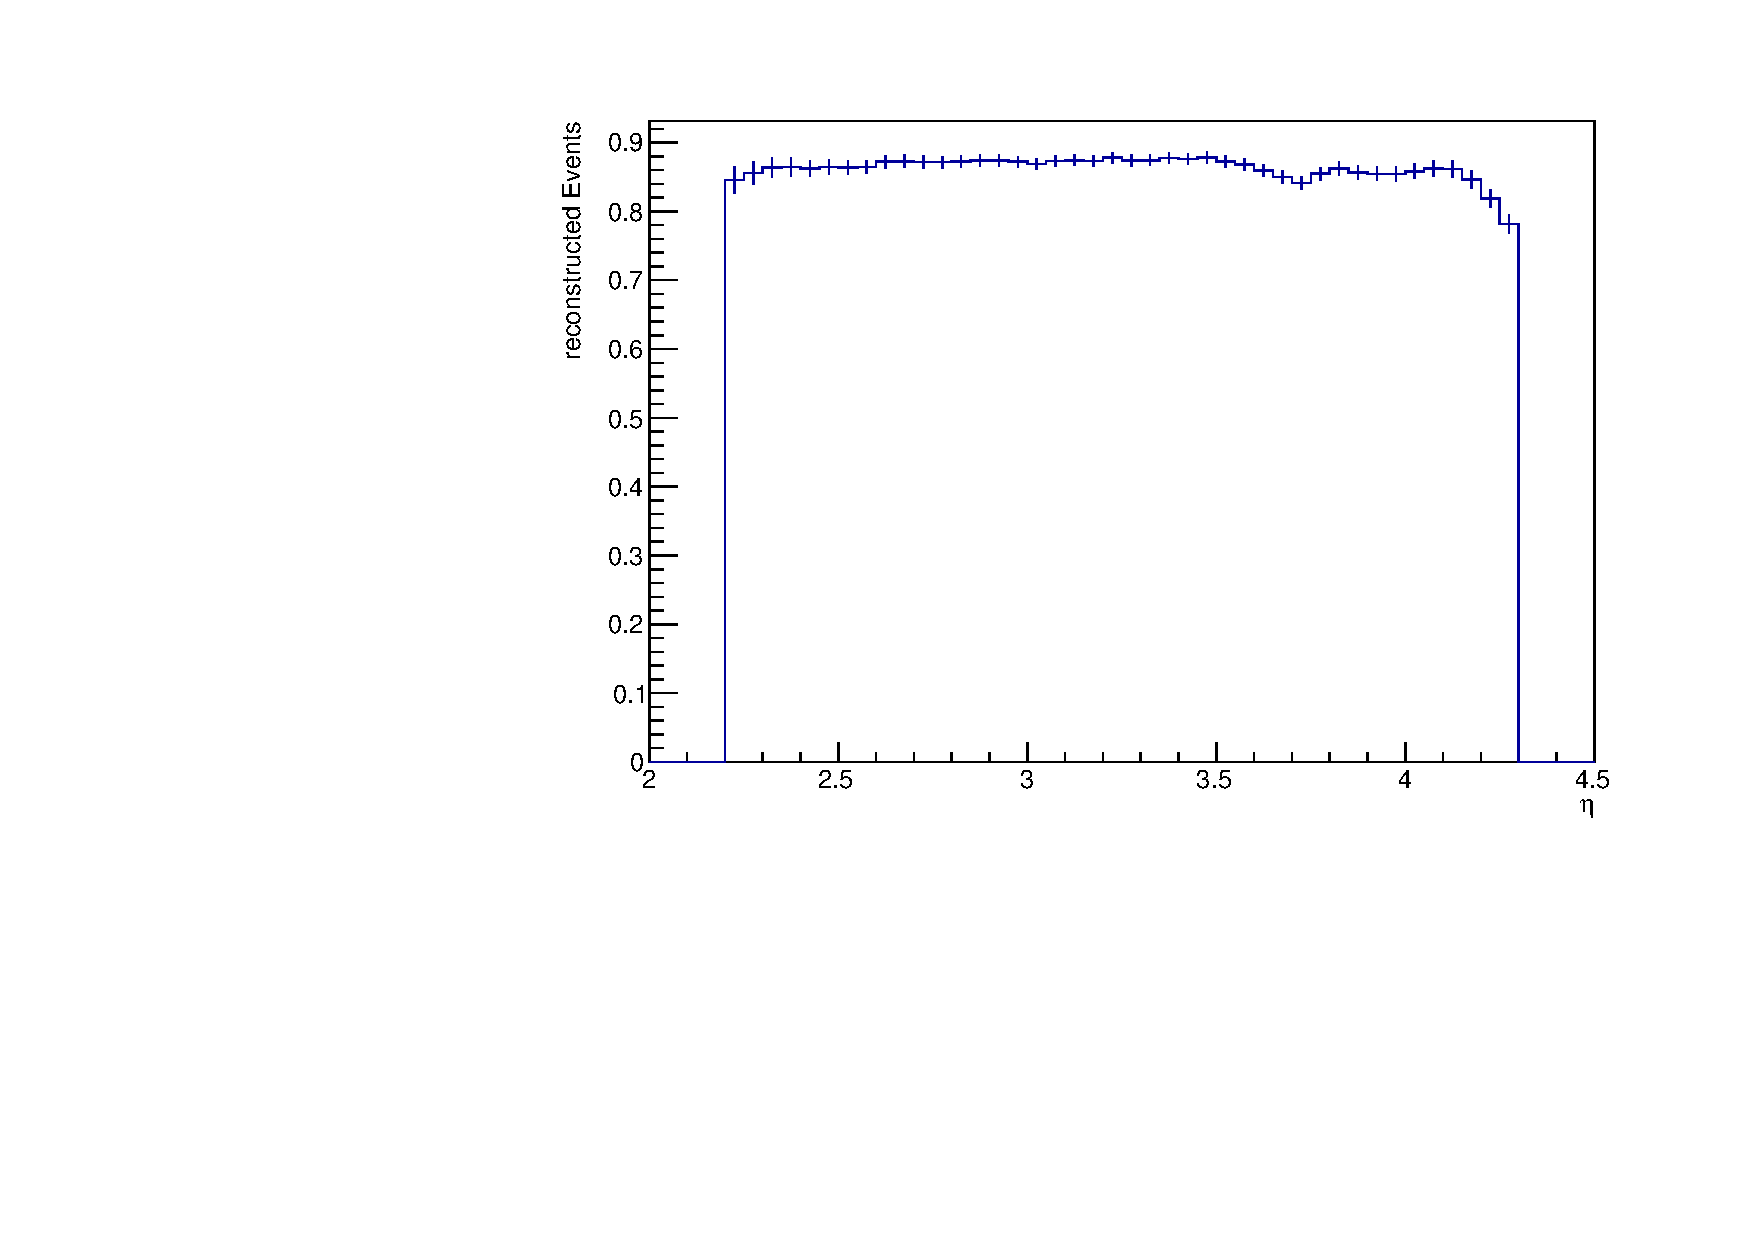
\includegraphics[width=0.9\textwidth]{up_pdf/tot/h_eta_reco_Pi.pdf}
\end{subfigure}
\end{figure}
\end{frame}
\begin{frame}{$K$-efficiency}
\begin{figure}
\begin{subfigure}{0.45\textwidth}
\includegraphics[width=0.9\textwidth]{up_pdf/tot/h_pt_reco_K.pdf}
\end{subfigure}
\begin{subfigure}{0.45\textwidth}
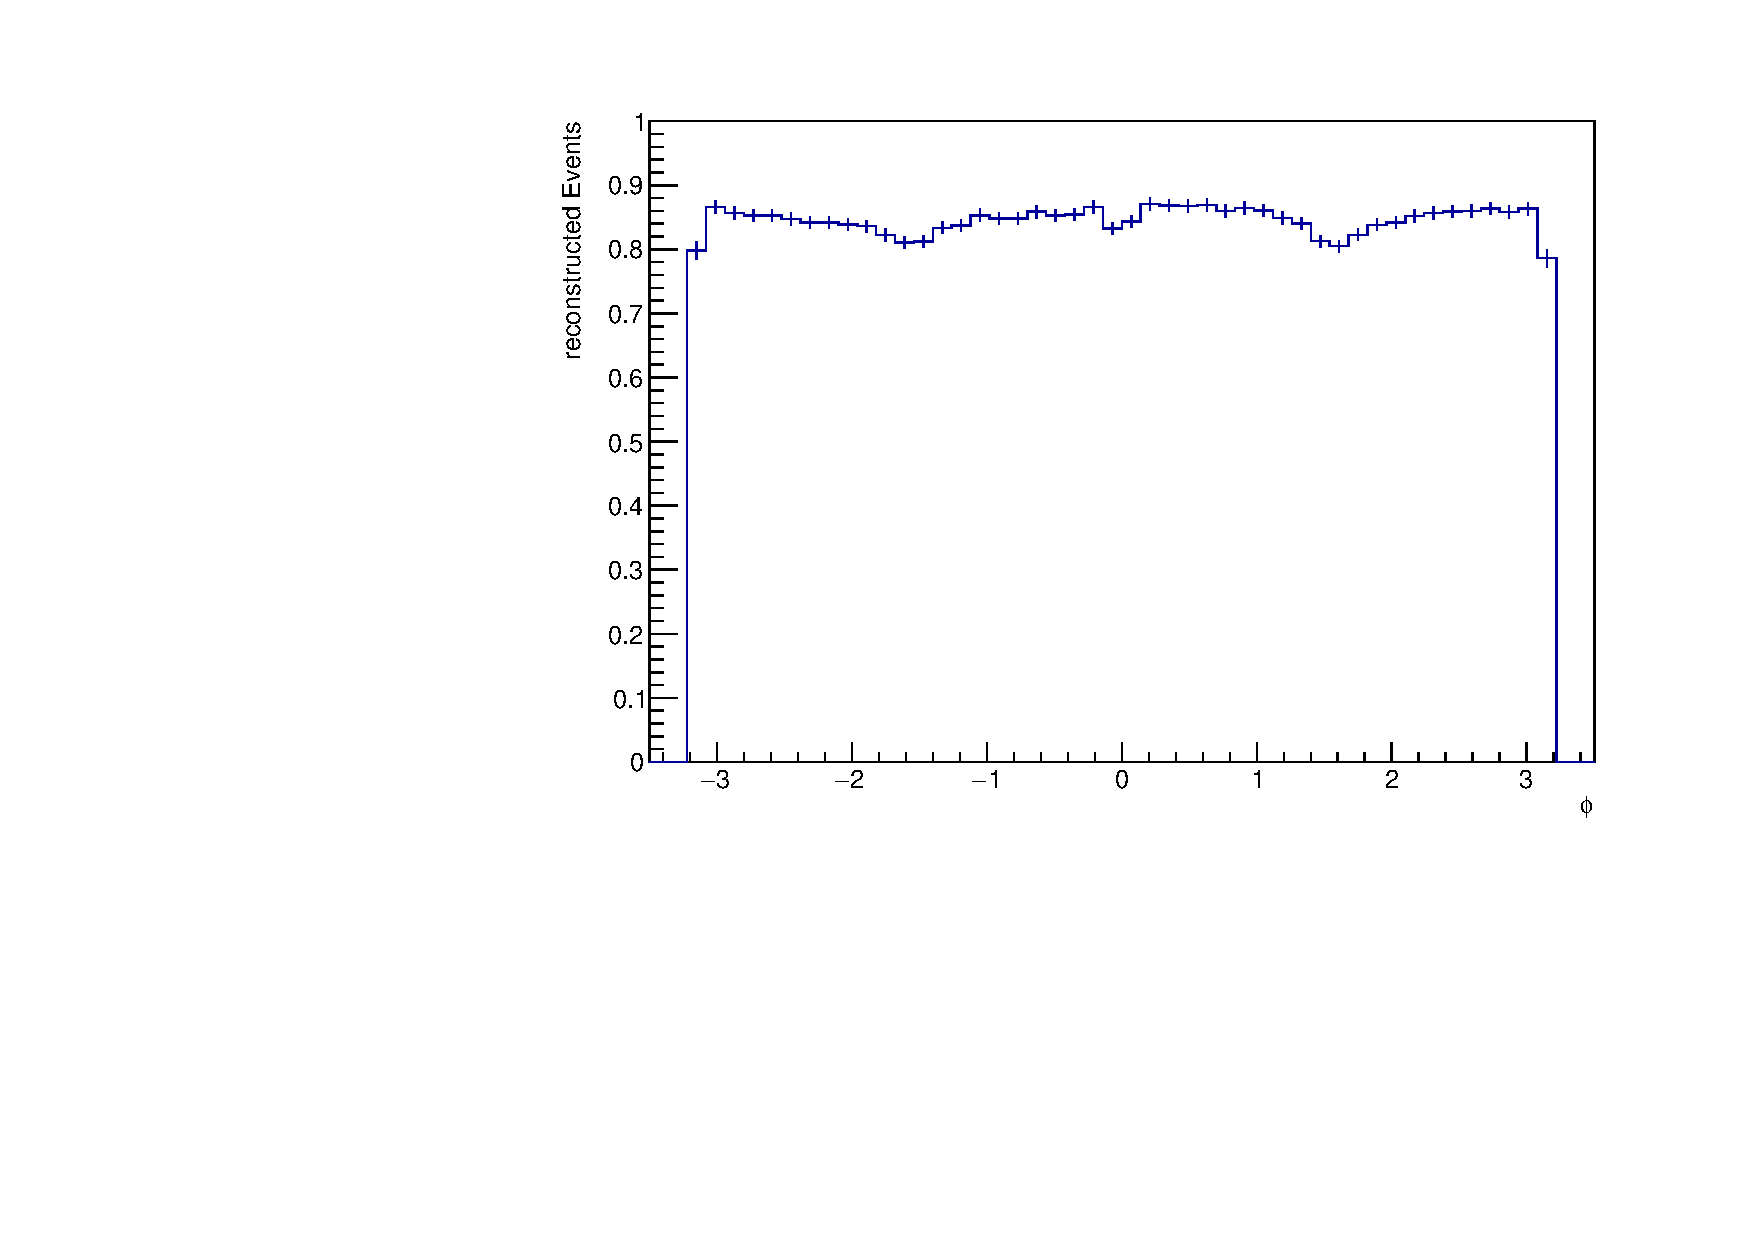
\includegraphics[width=0.9\textwidth]{up_pdf/tot/h_phi_reco_K.pdf}
\end{subfigure}
\begin{subfigure}{0.45\textwidth}
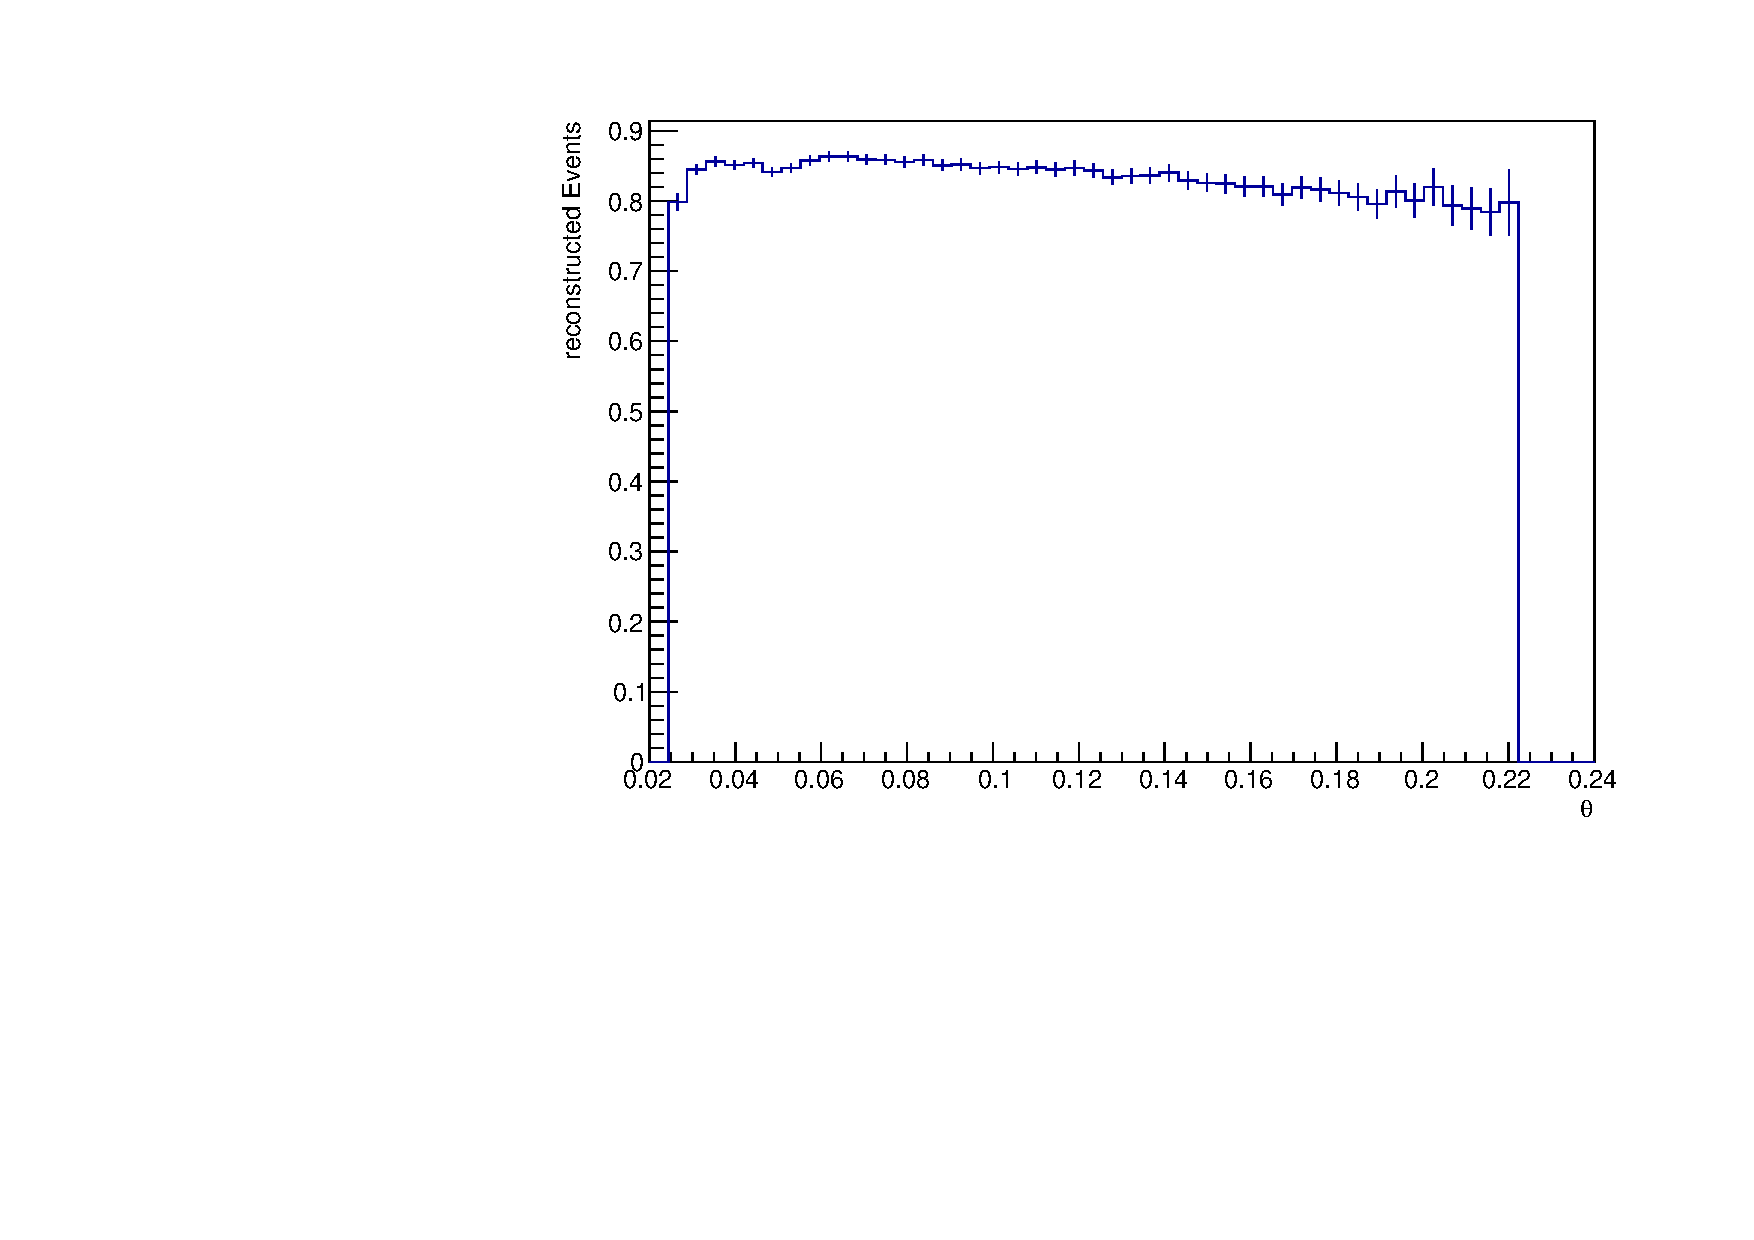
\includegraphics[width=0.9\textwidth]{up_pdf/tot/h_theta_reco_K.pdf}
\end{subfigure}
\begin{subfigure}{0.45\textwidth}
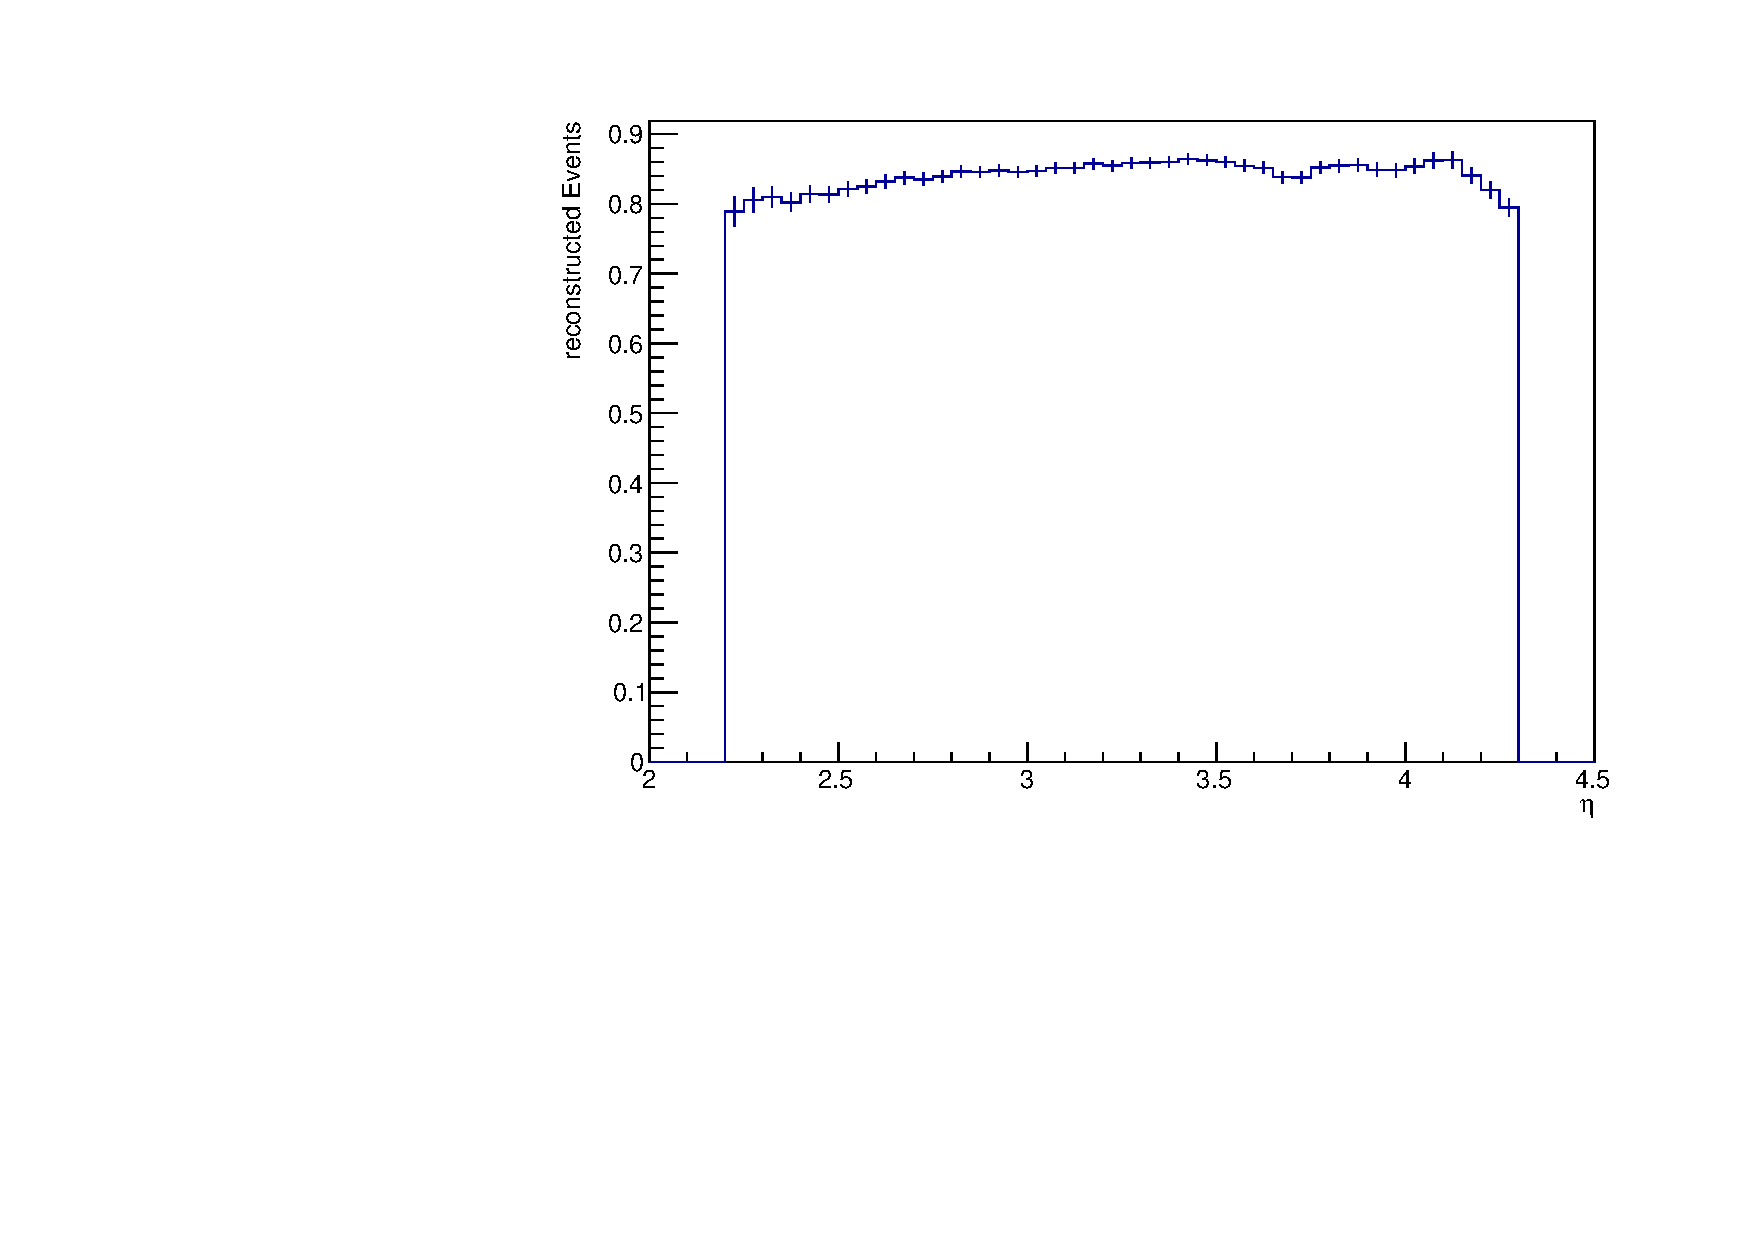
\includegraphics[width=0.9\textwidth]{up_pdf/tot/h_eta_reco_K.pdf}
\end{subfigure}
\end{figure}
\end{frame}
\begin{frame}{soft $\pi$-efficiency}
\begin{figure}
\begin{subfigure}{0.45\textwidth}
\includegraphics[width=0.9\textwidth]{up_pdf/tot/h_pt_reco_SPi.pdf}
\end{subfigure}
\begin{subfigure}{0.45\textwidth}
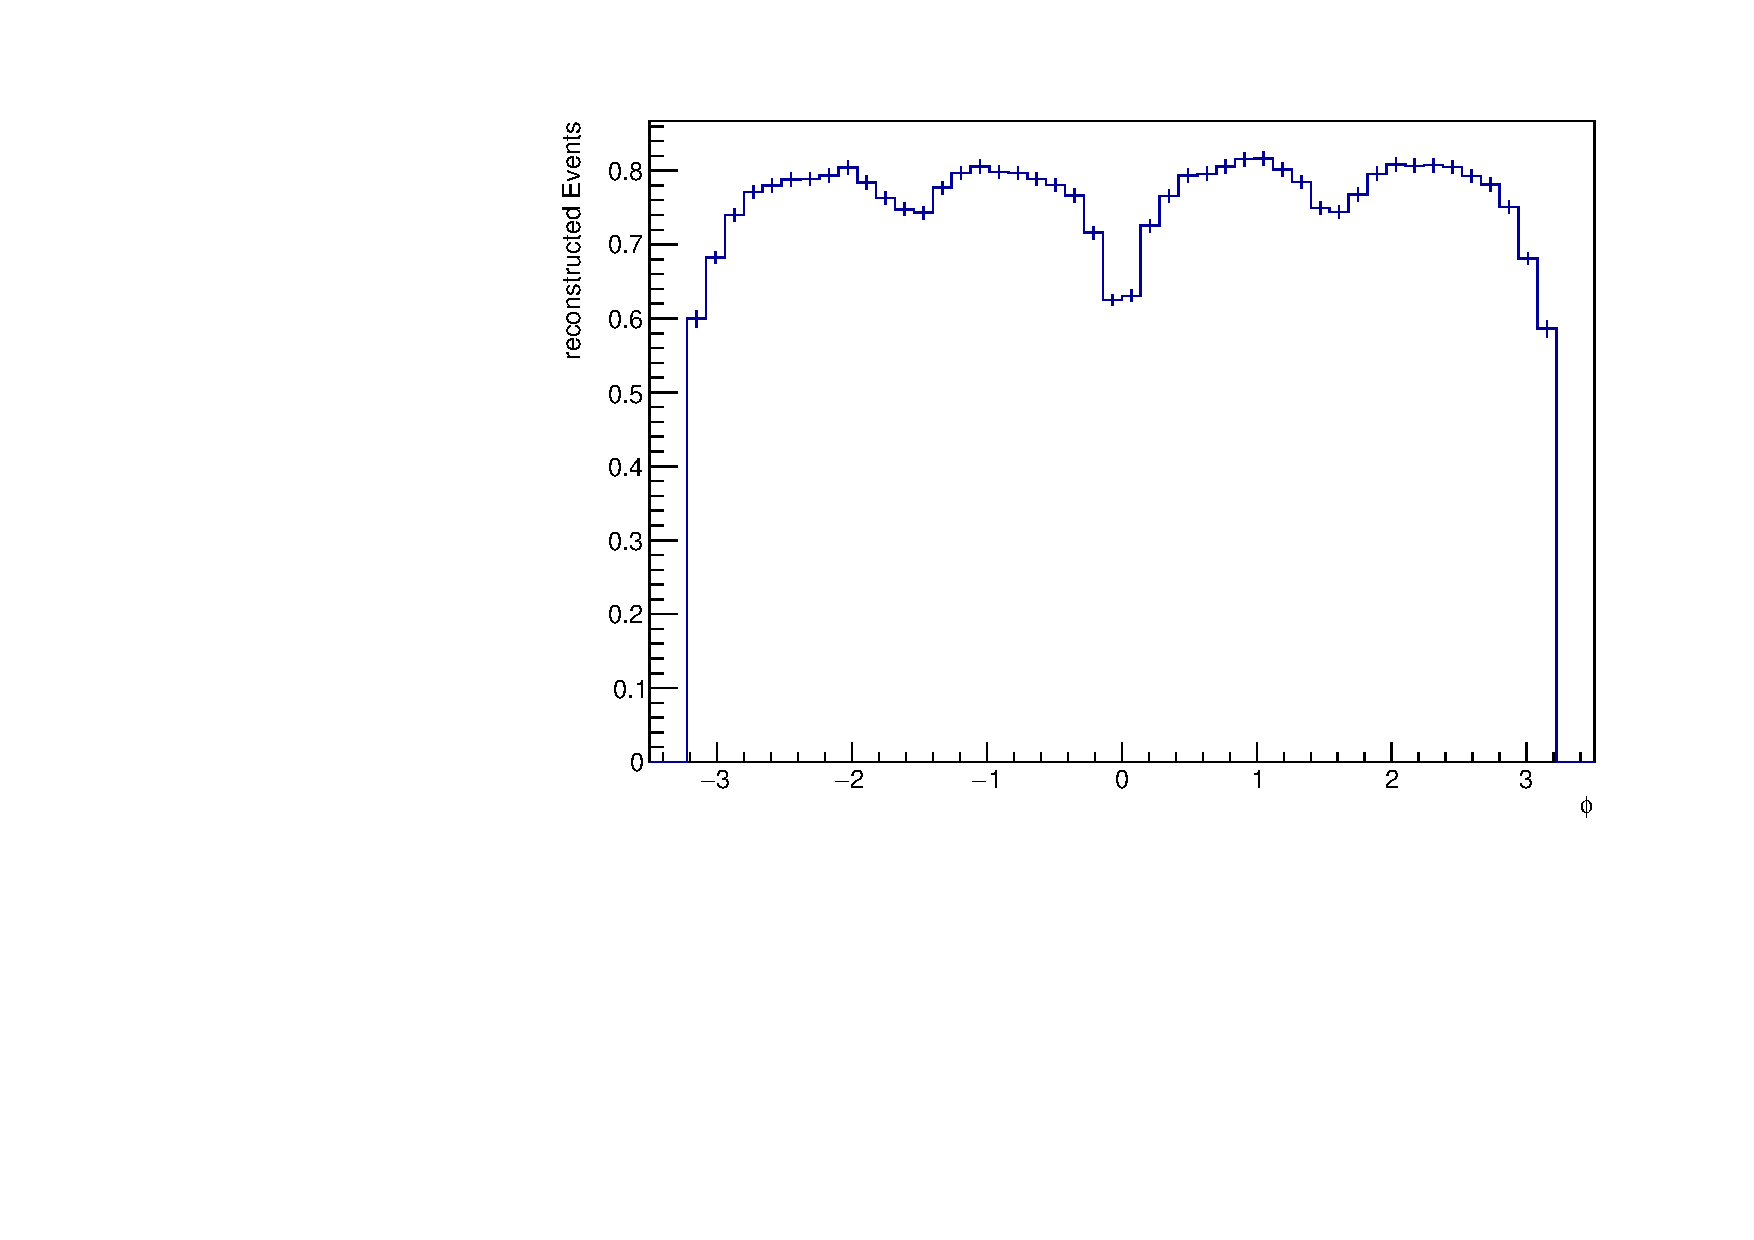
\includegraphics[width=0.9\textwidth]{up_pdf/tot/h_phi_reco_SPi.pdf}
\end{subfigure}
\begin{subfigure}{0.45\textwidth}
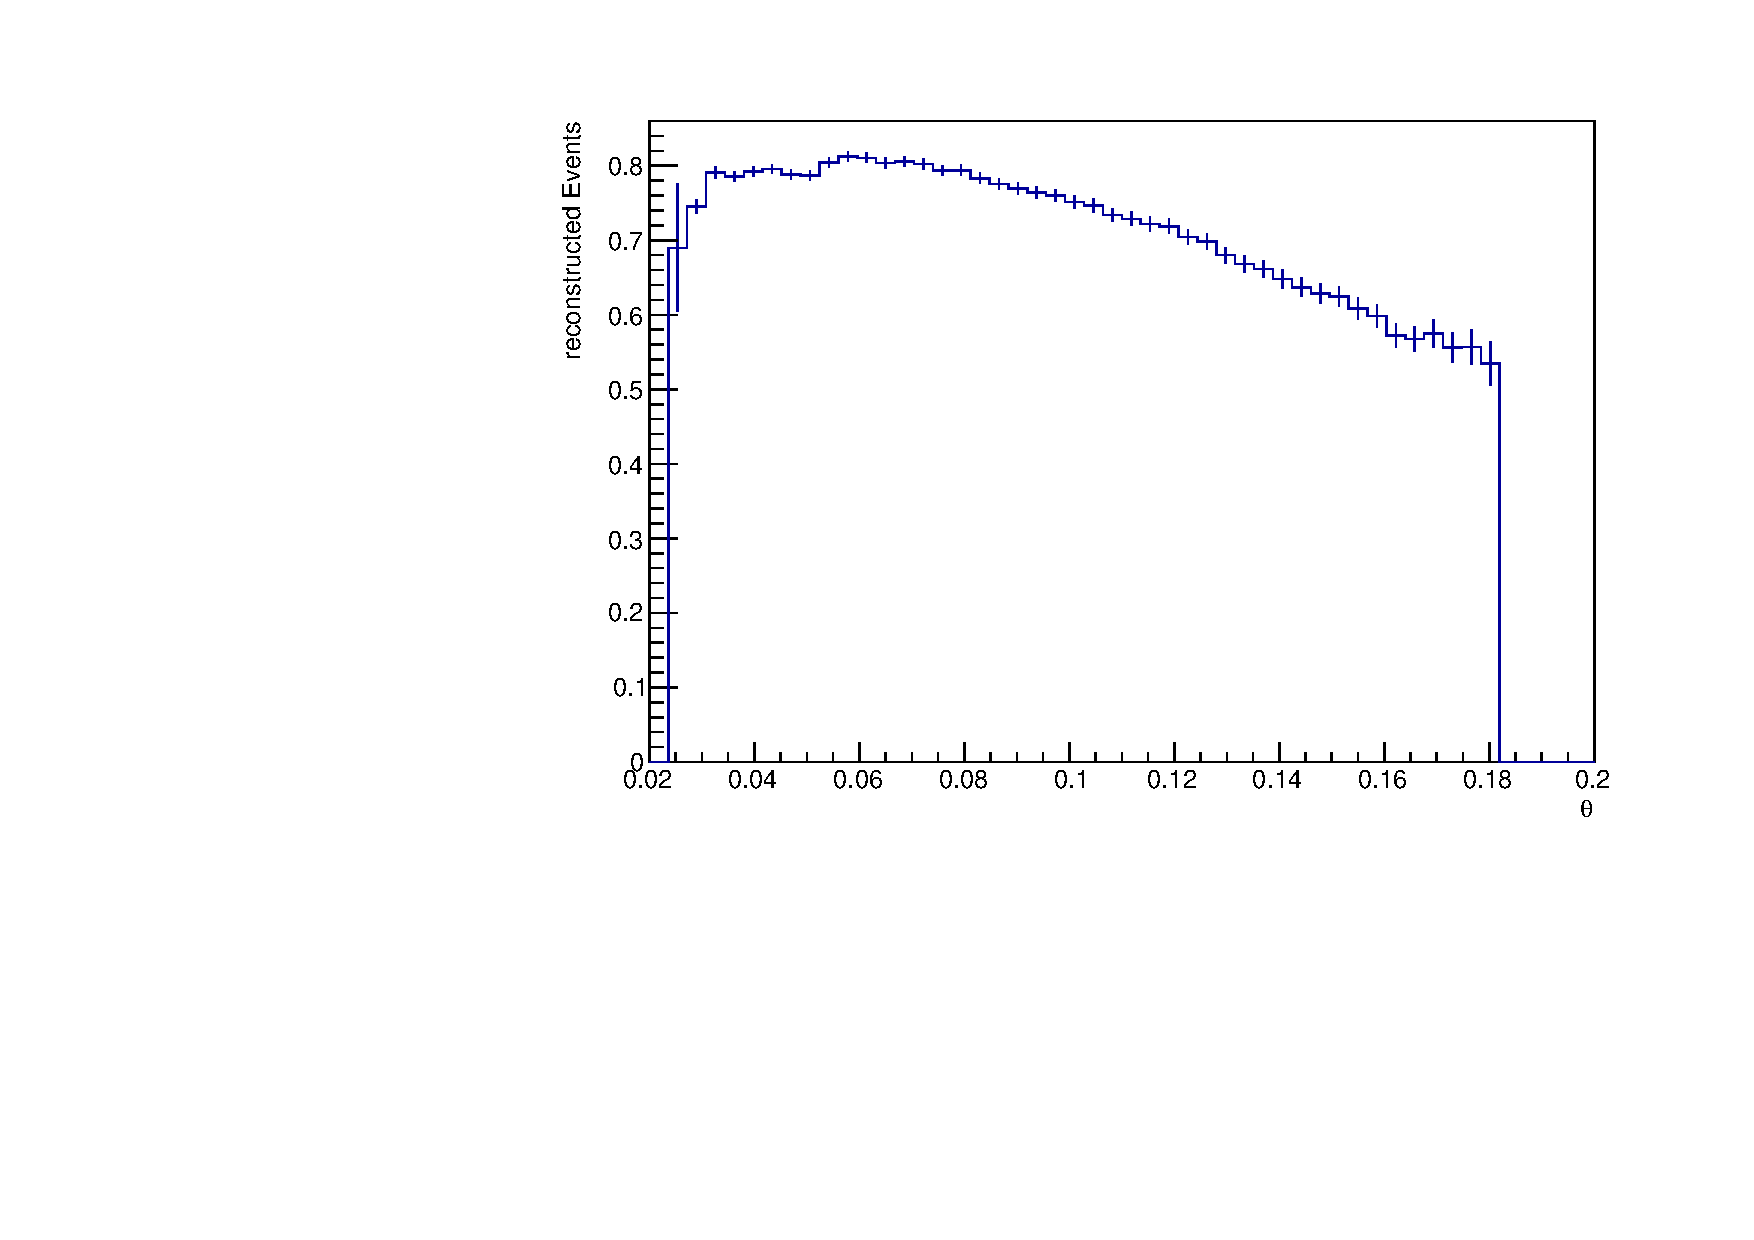
\includegraphics[width=0.9\textwidth]{up_pdf/tot/h_theta_reco_SPi.pdf}
\end{subfigure}
\begin{subfigure}{0.45\textwidth}
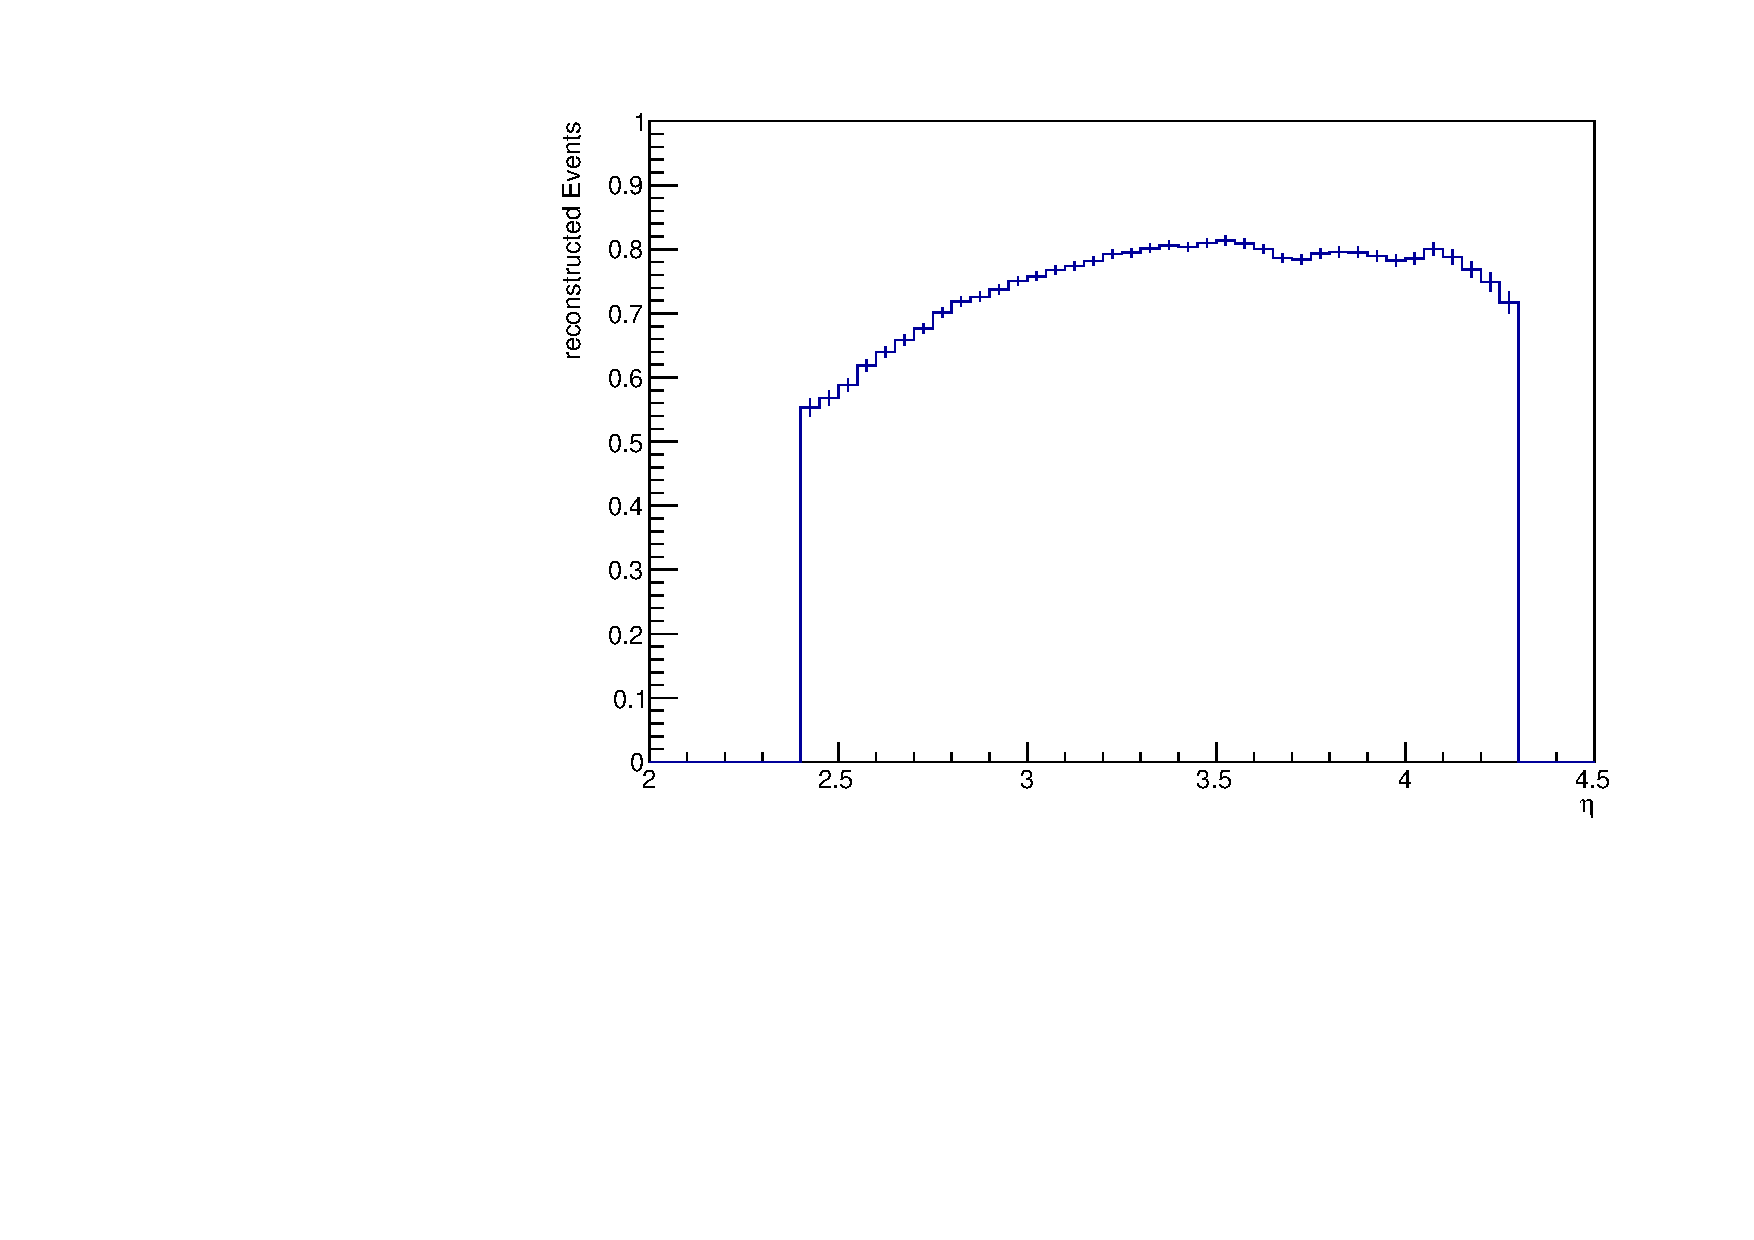
\includegraphics[width=0.9\textwidth]{up_pdf/tot/h_eta_reco_SPi.pdf}
\end{subfigure}
\end{figure}
\end{frame}
\begin{frame}{$D^0$-efficiency}
\begin{figure}
\begin{subfigure}{0.45\textwidth}
\includegraphics[width=0.9\textwidth]{up_pdf/tot/h_pt_reco_D0.pdf}
\end{subfigure}
\begin{subfigure}{0.45\textwidth}
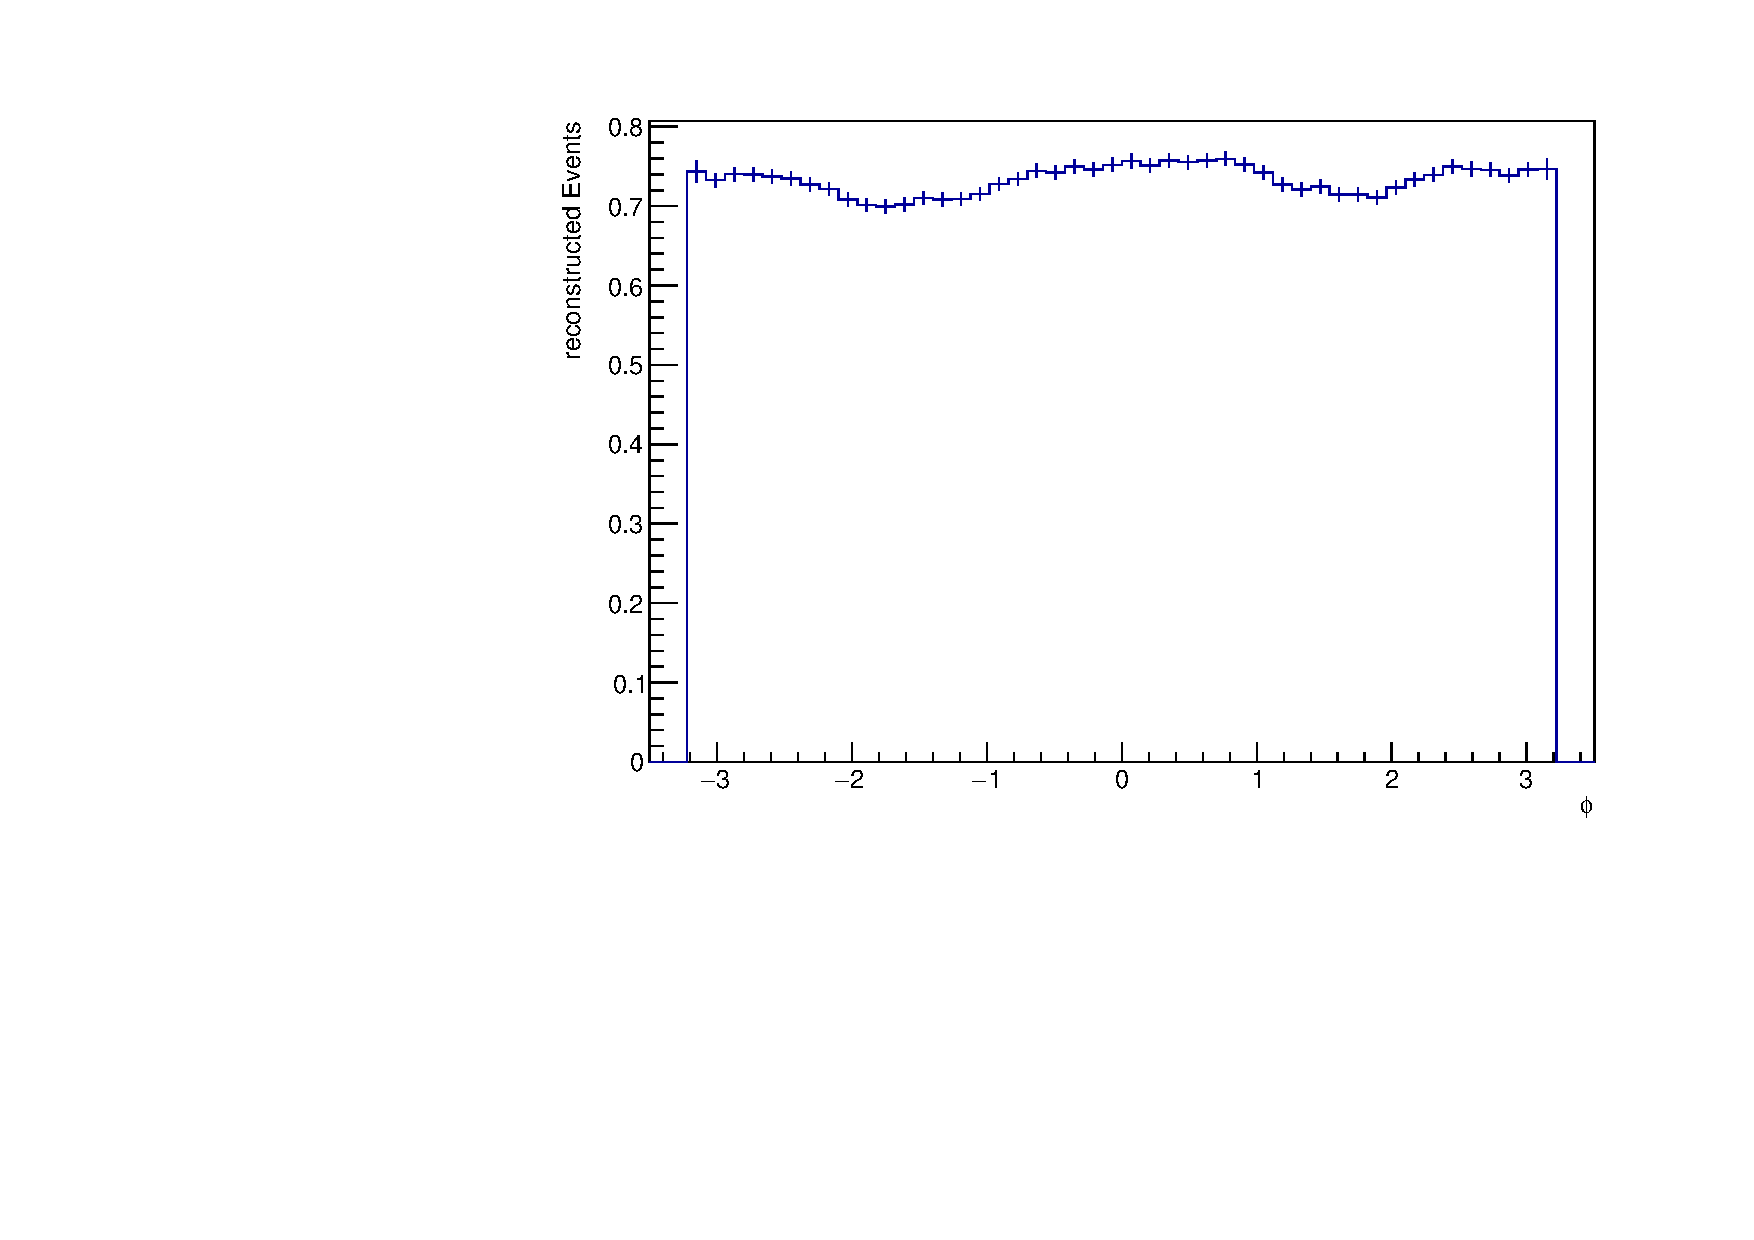
\includegraphics[width=0.9\textwidth]{up_pdf/tot/h_phi_reco_D0.pdf}
\end{subfigure}
\begin{subfigure}{0.45\textwidth}
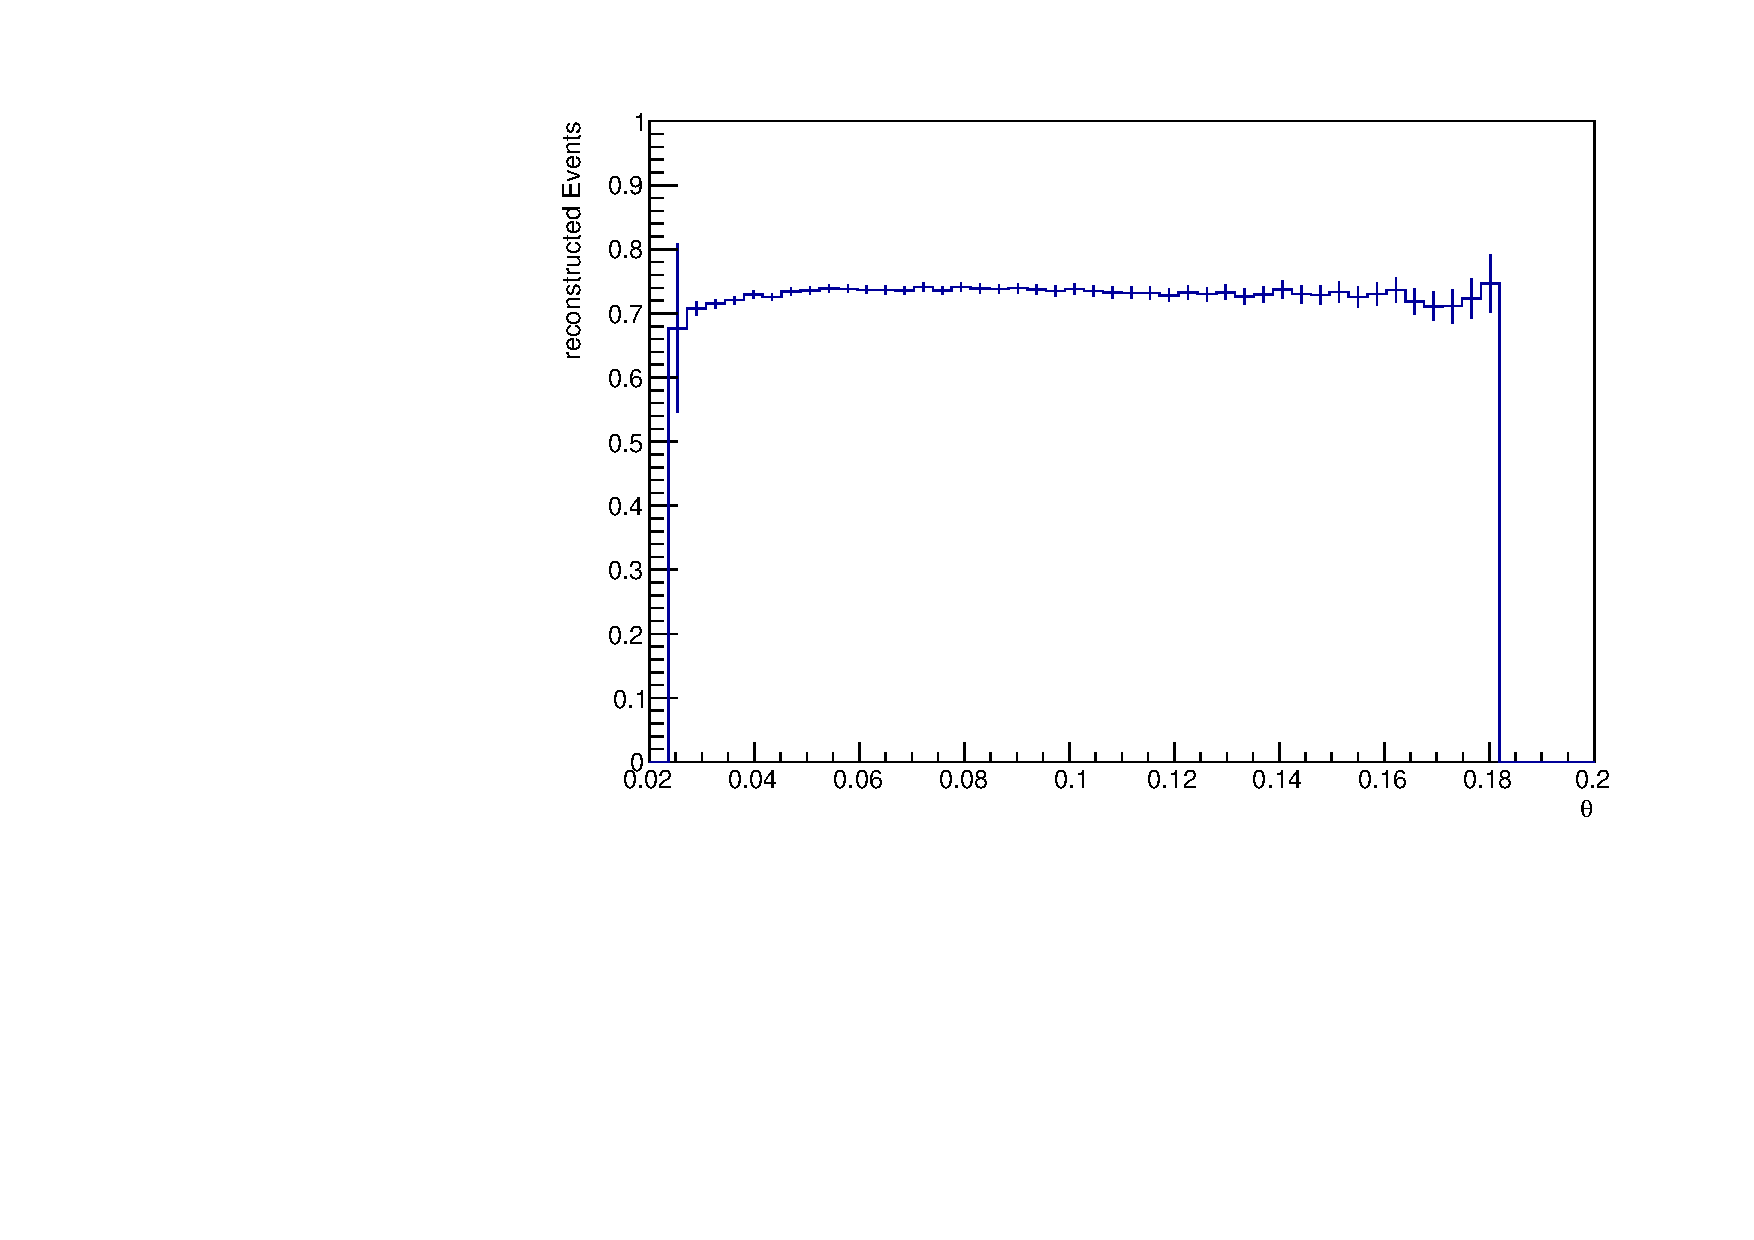
\includegraphics[width=0.9\textwidth]{up_pdf/tot/h_theta_reco_D0.pdf}
\end{subfigure}
\begin{subfigure}{0.45\textwidth}
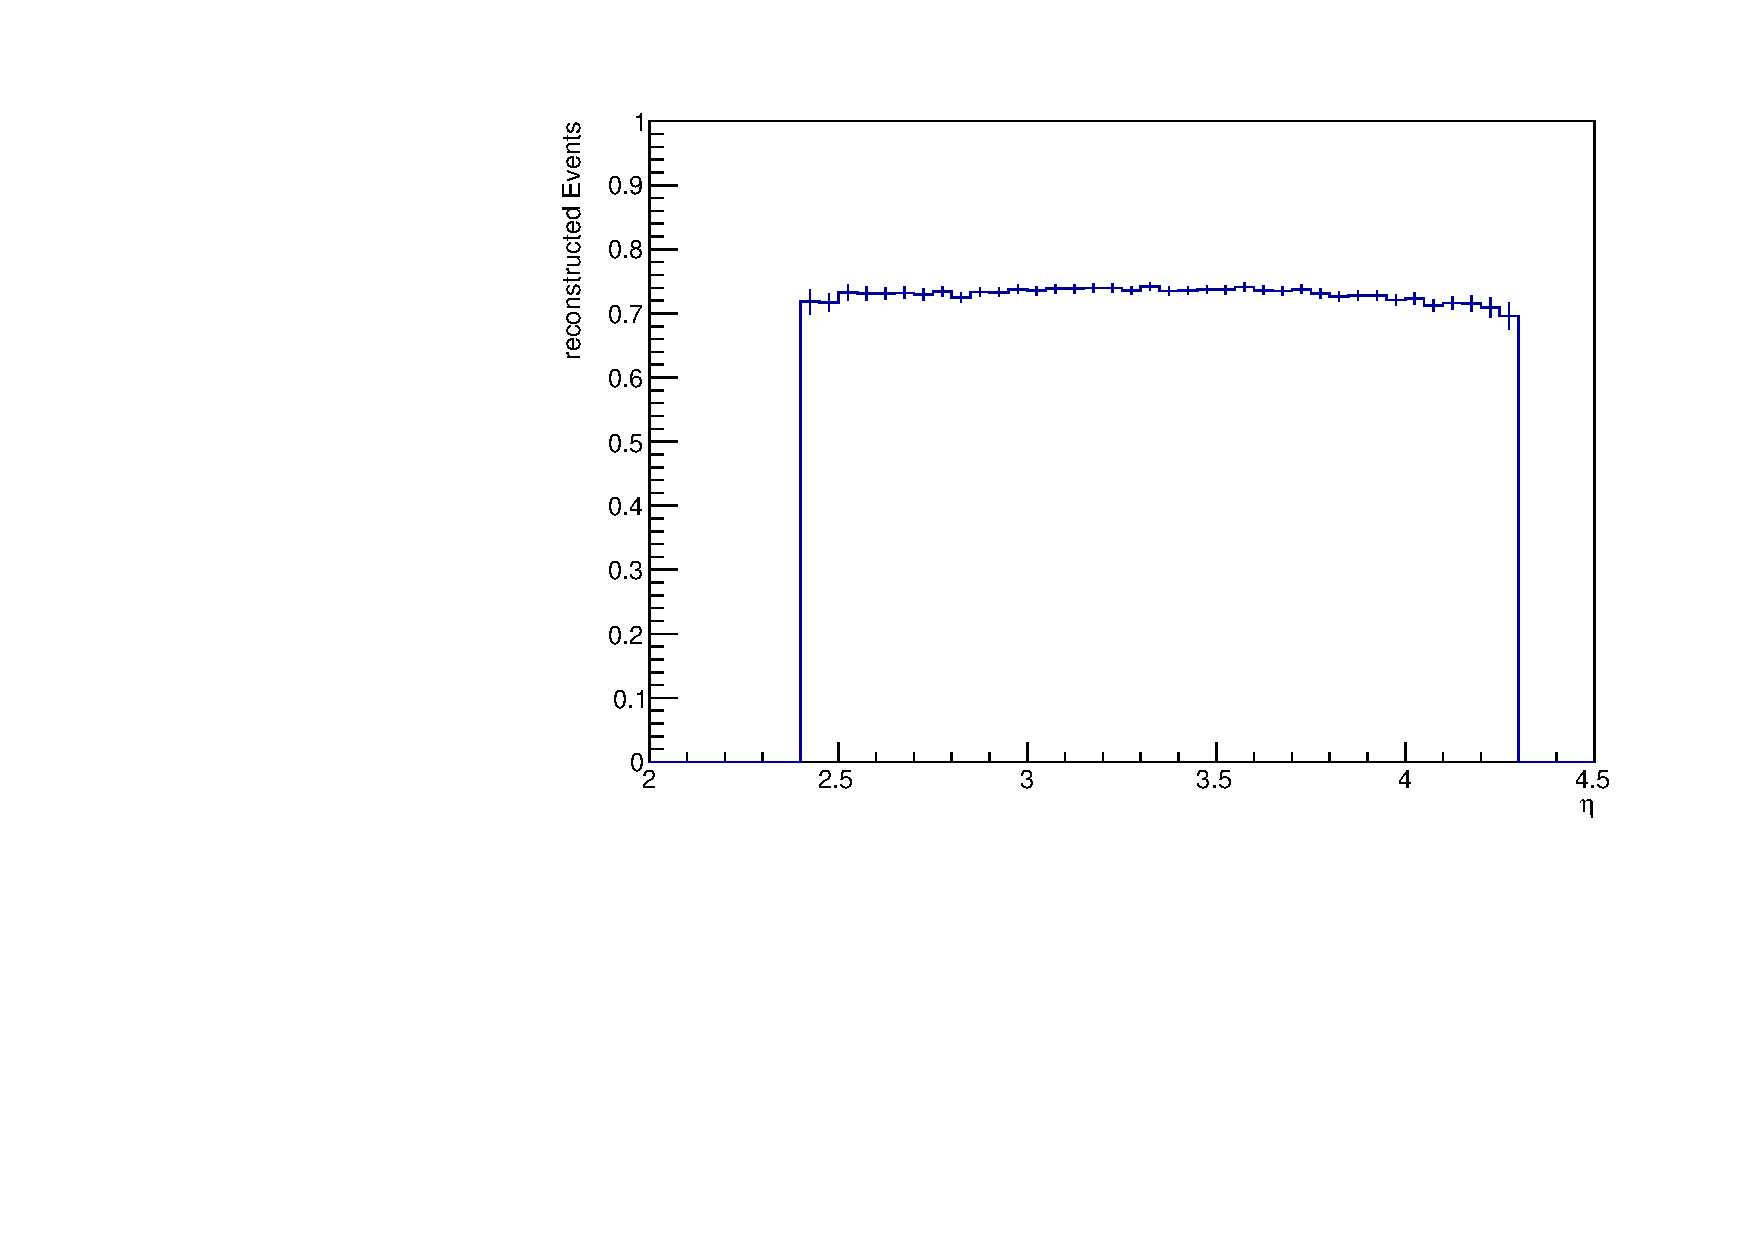
\includegraphics[width=0.9\textwidth]{up_pdf/tot/h_eta_reco_D0.pdf}
\end{subfigure}
\end{figure}
\end{frame}
\begin{frame}{$D^*$-efficiency}
\begin{figure}
\begin{subfigure}{0.45\textwidth}
\includegraphics[width=0.9\textwidth]{up_pdf/tot/h_pt_reco_Dst.pdf}
\end{subfigure}
\begin{subfigure}{0.45\textwidth}
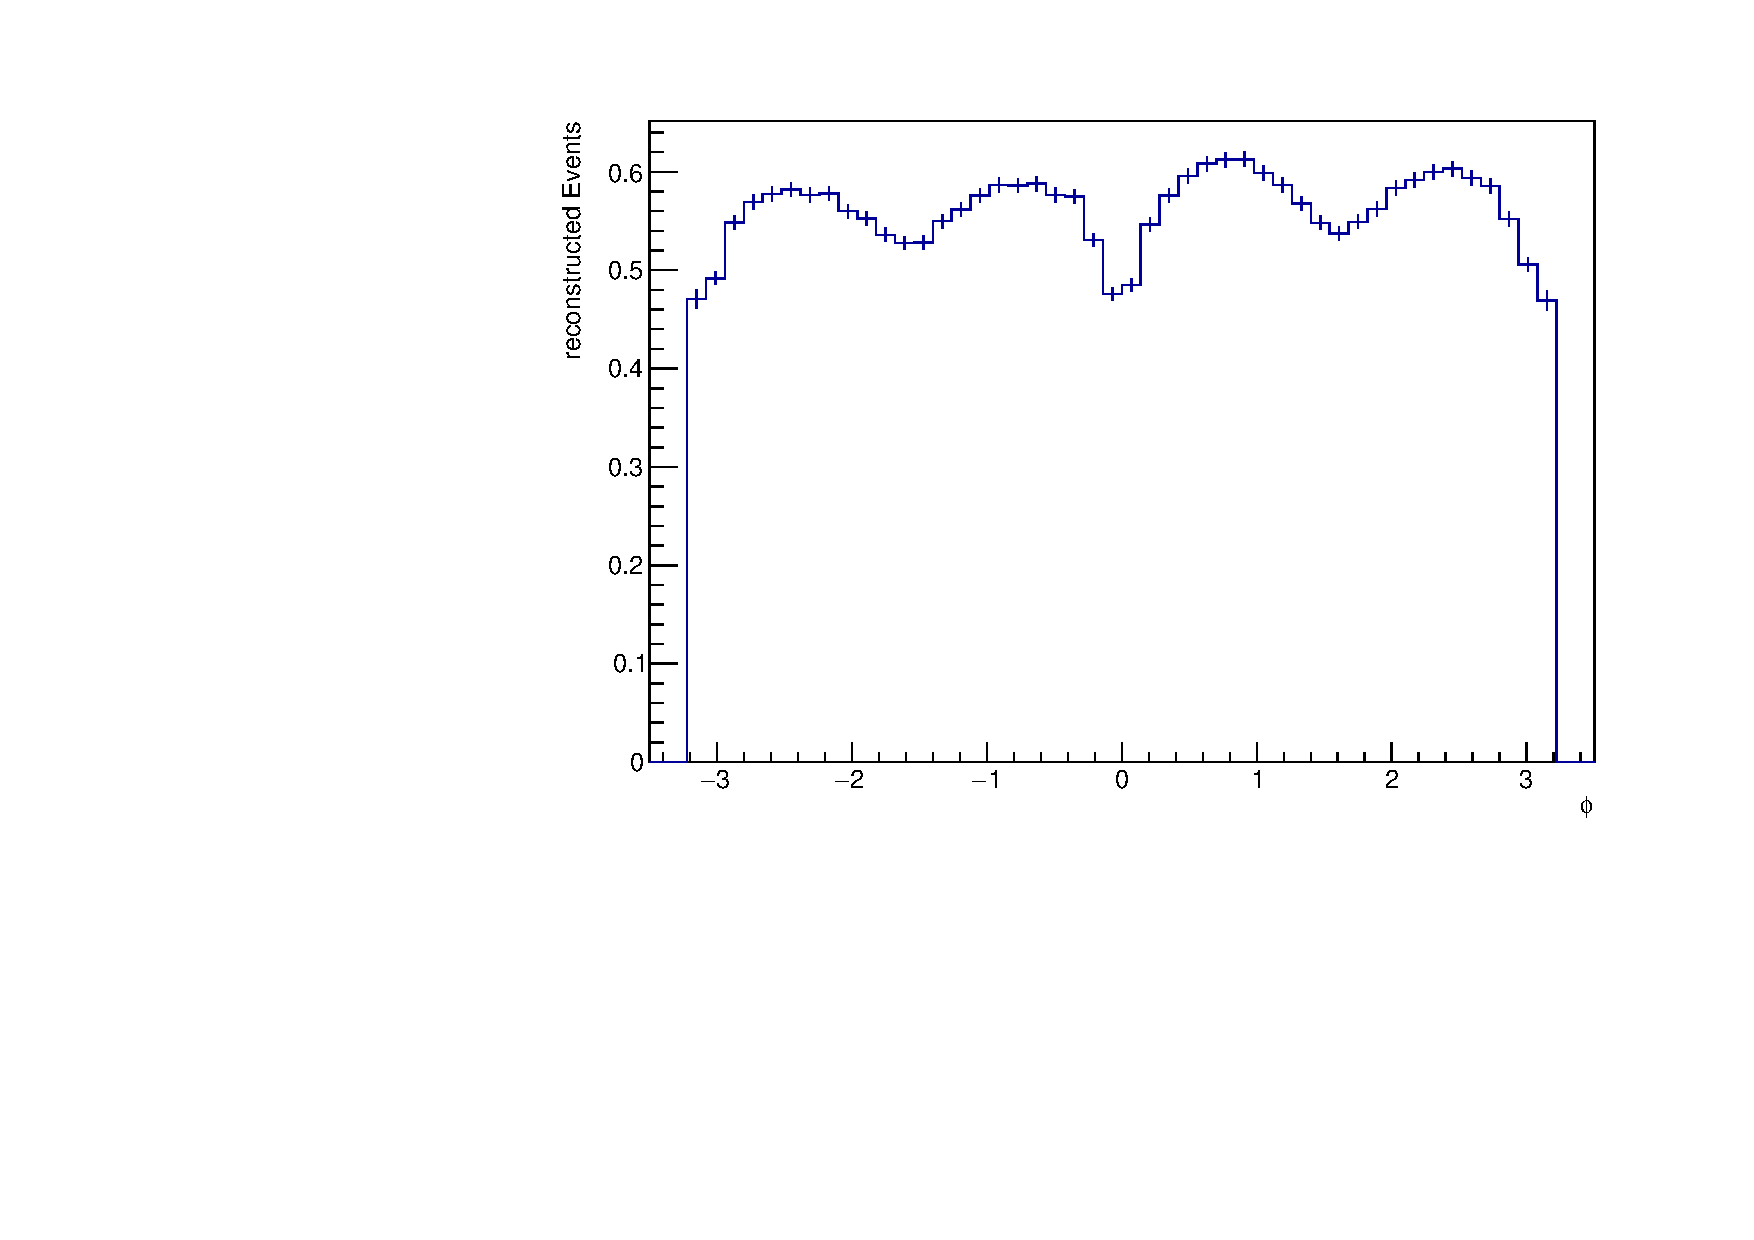
\includegraphics[width=0.9\textwidth]{up_pdf/tot/h_phi_reco_Dst.pdf}
\end{subfigure}
\begin{subfigure}{0.45\textwidth}
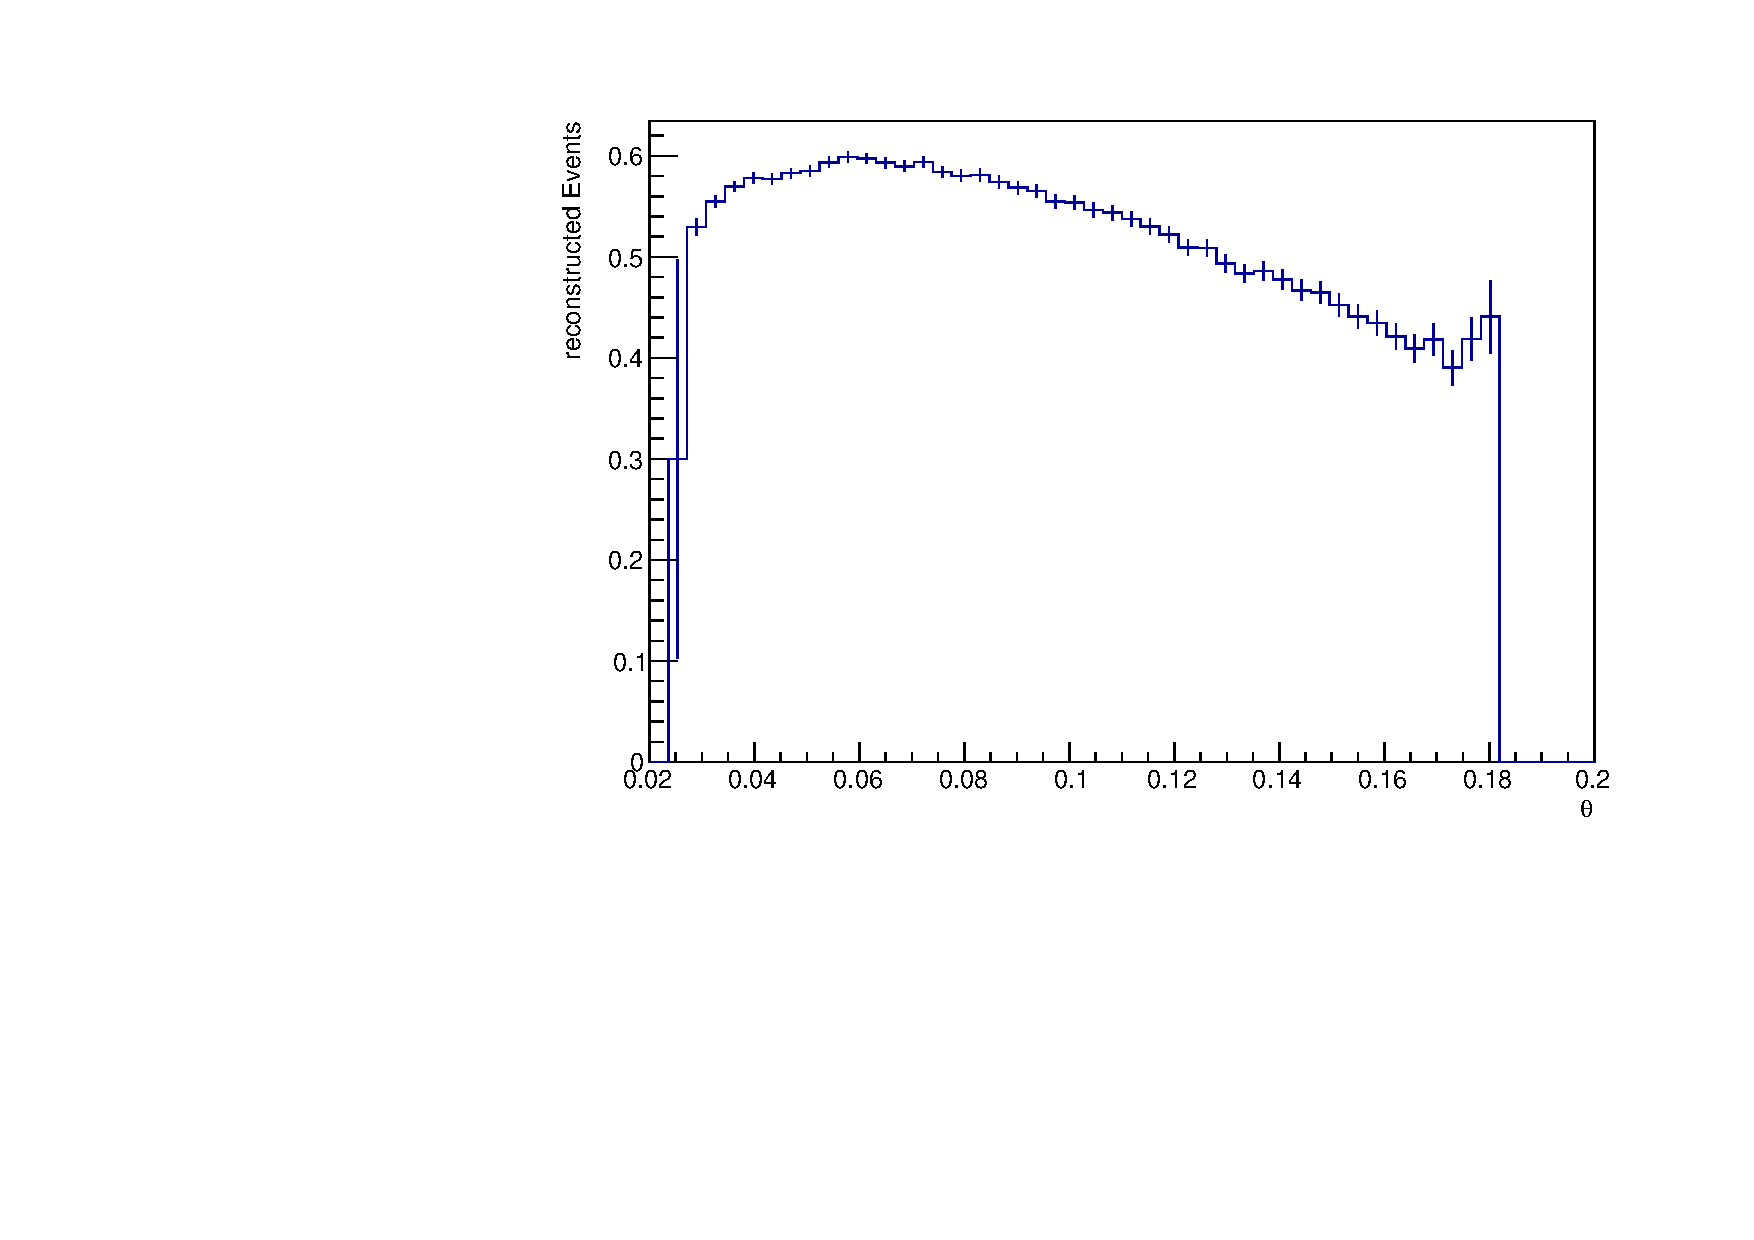
\includegraphics[width=0.9\textwidth]{up_pdf/tot/h_theta_reco_Dst.pdf}
\end{subfigure}
\begin{subfigure}{0.45\textwidth}
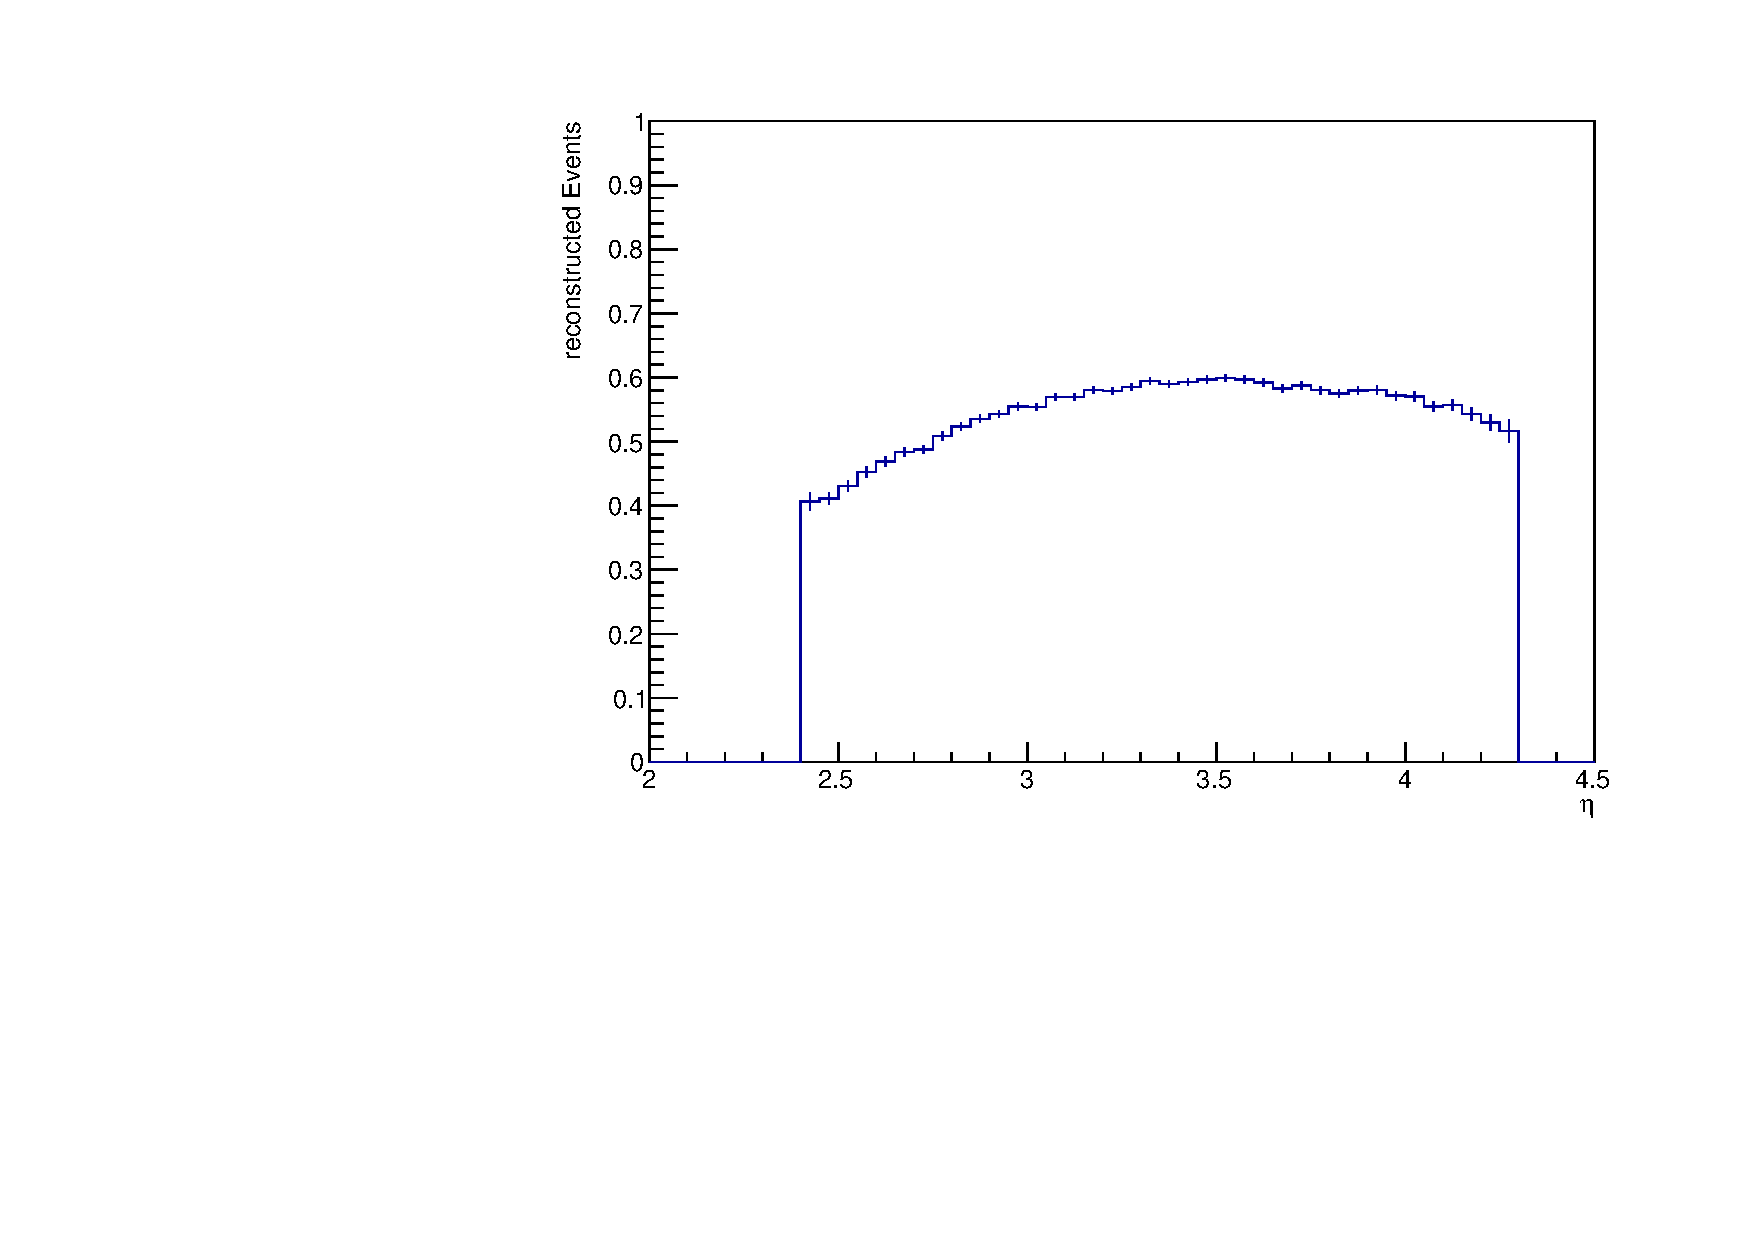
\includegraphics[width=0.9\textwidth]{up_pdf/tot/h_eta_reco_Dst.pdf}
\end{subfigure}
\end{figure}
\end{frame}
\begin{frame}
\begin{LARGE}
\textbf{Charge: +}
\end{LARGE}
\end{frame}
\begin{frame}{$\pi$-efficiency}
\begin{figure}
\begin{subfigure}{0.45\textwidth}
\includegraphics[width=0.9\textwidth]{up_pdf/pos/h_pt_reco_Pi_pos.pdf}
\end{subfigure}
\begin{subfigure}{0.45\textwidth}
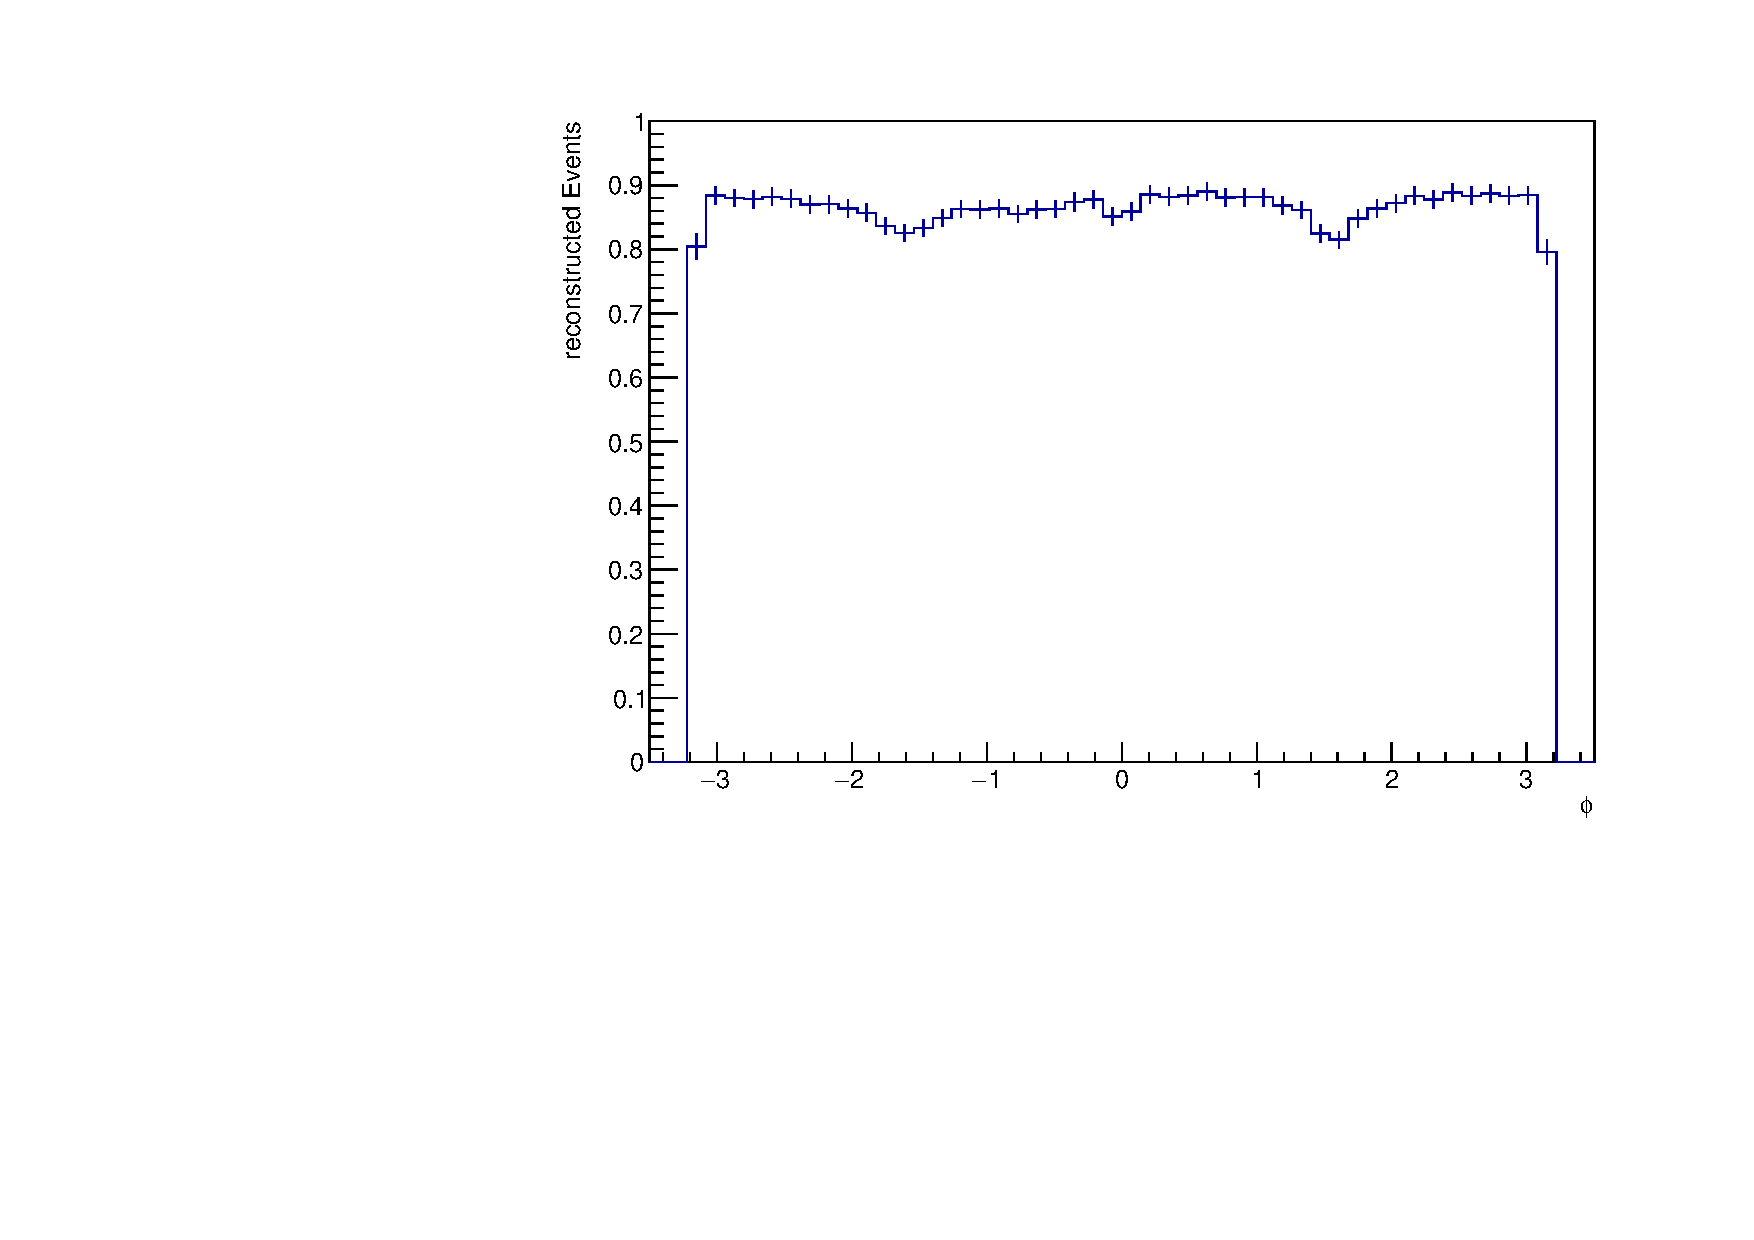
\includegraphics[width=0.9\textwidth]{up_pdf/pos/h_phi_reco_Pi_pos.pdf}
\end{subfigure}
\begin{subfigure}{0.45\textwidth}
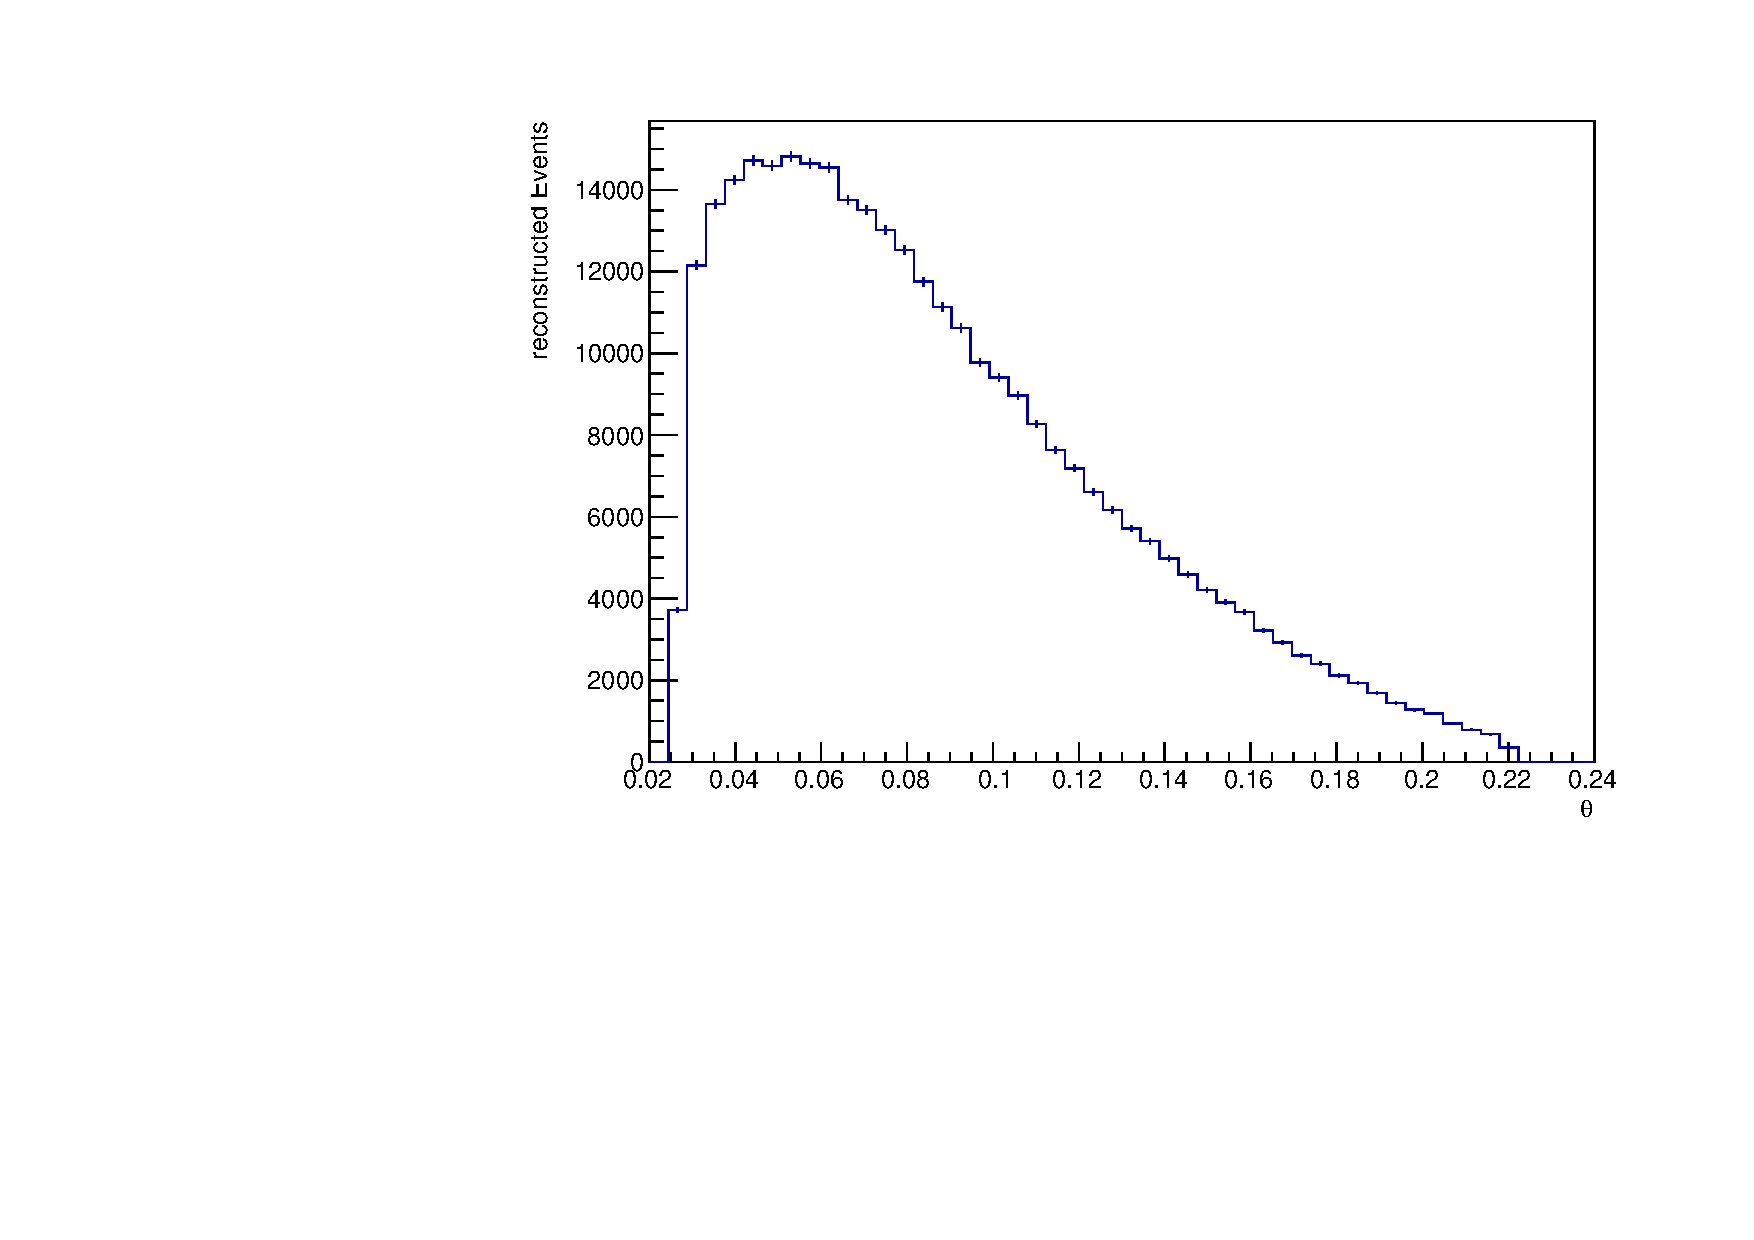
\includegraphics[width=0.9\textwidth]{up_pdf/pos/h_theta_reco_Pi_pos.pdf}
\end{subfigure}
\begin{subfigure}{0.45\textwidth}
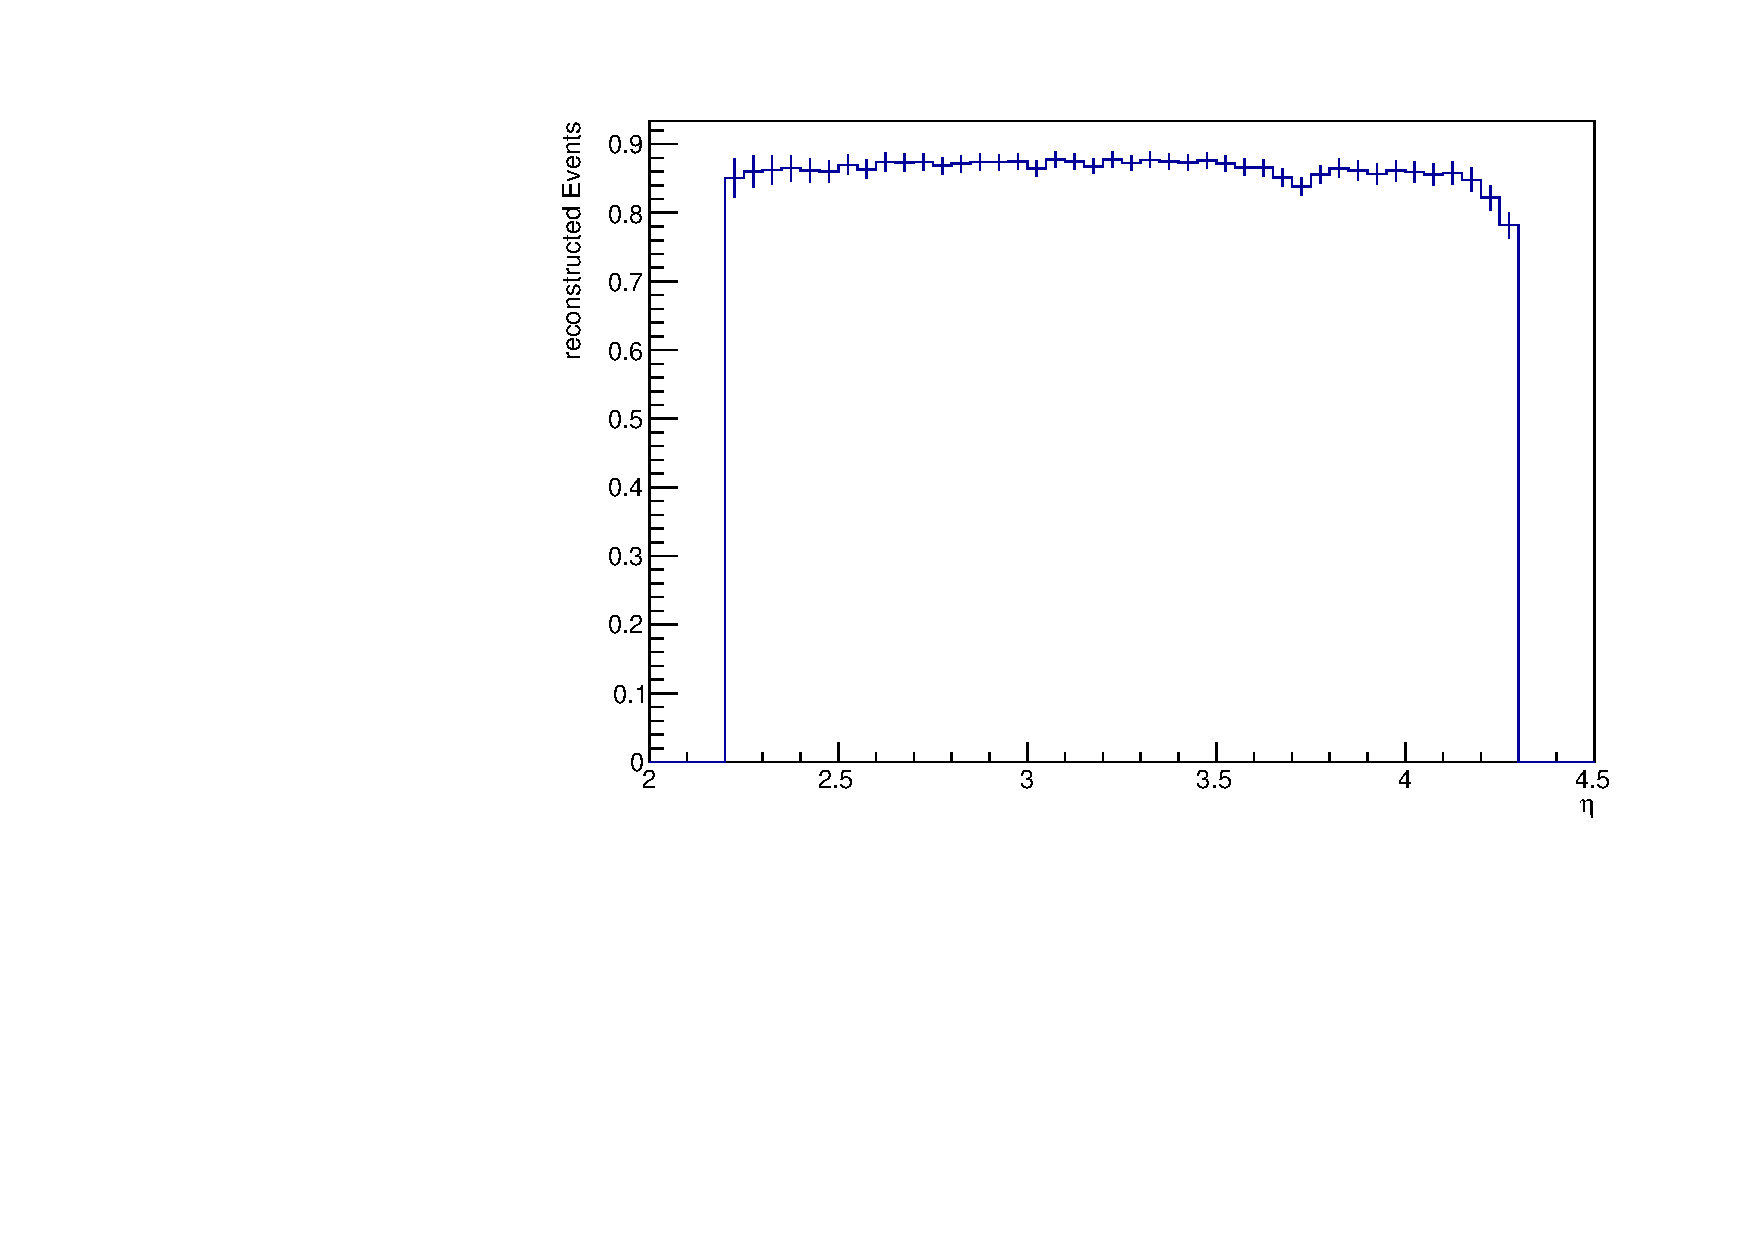
\includegraphics[width=0.9\textwidth]{up_pdf/pos/h_eta_reco_Pi_pos.pdf}
\end{subfigure}
\end{figure}
\end{frame}
\begin{frame}{$K$-efficiency}
\begin{figure}
\begin{subfigure}{0.45\textwidth}
\includegraphics[width=0.9\textwidth]{up_pdf/pos/h_pt_reco_K_pos.pdf}
\end{subfigure}
\begin{subfigure}{0.45\textwidth}
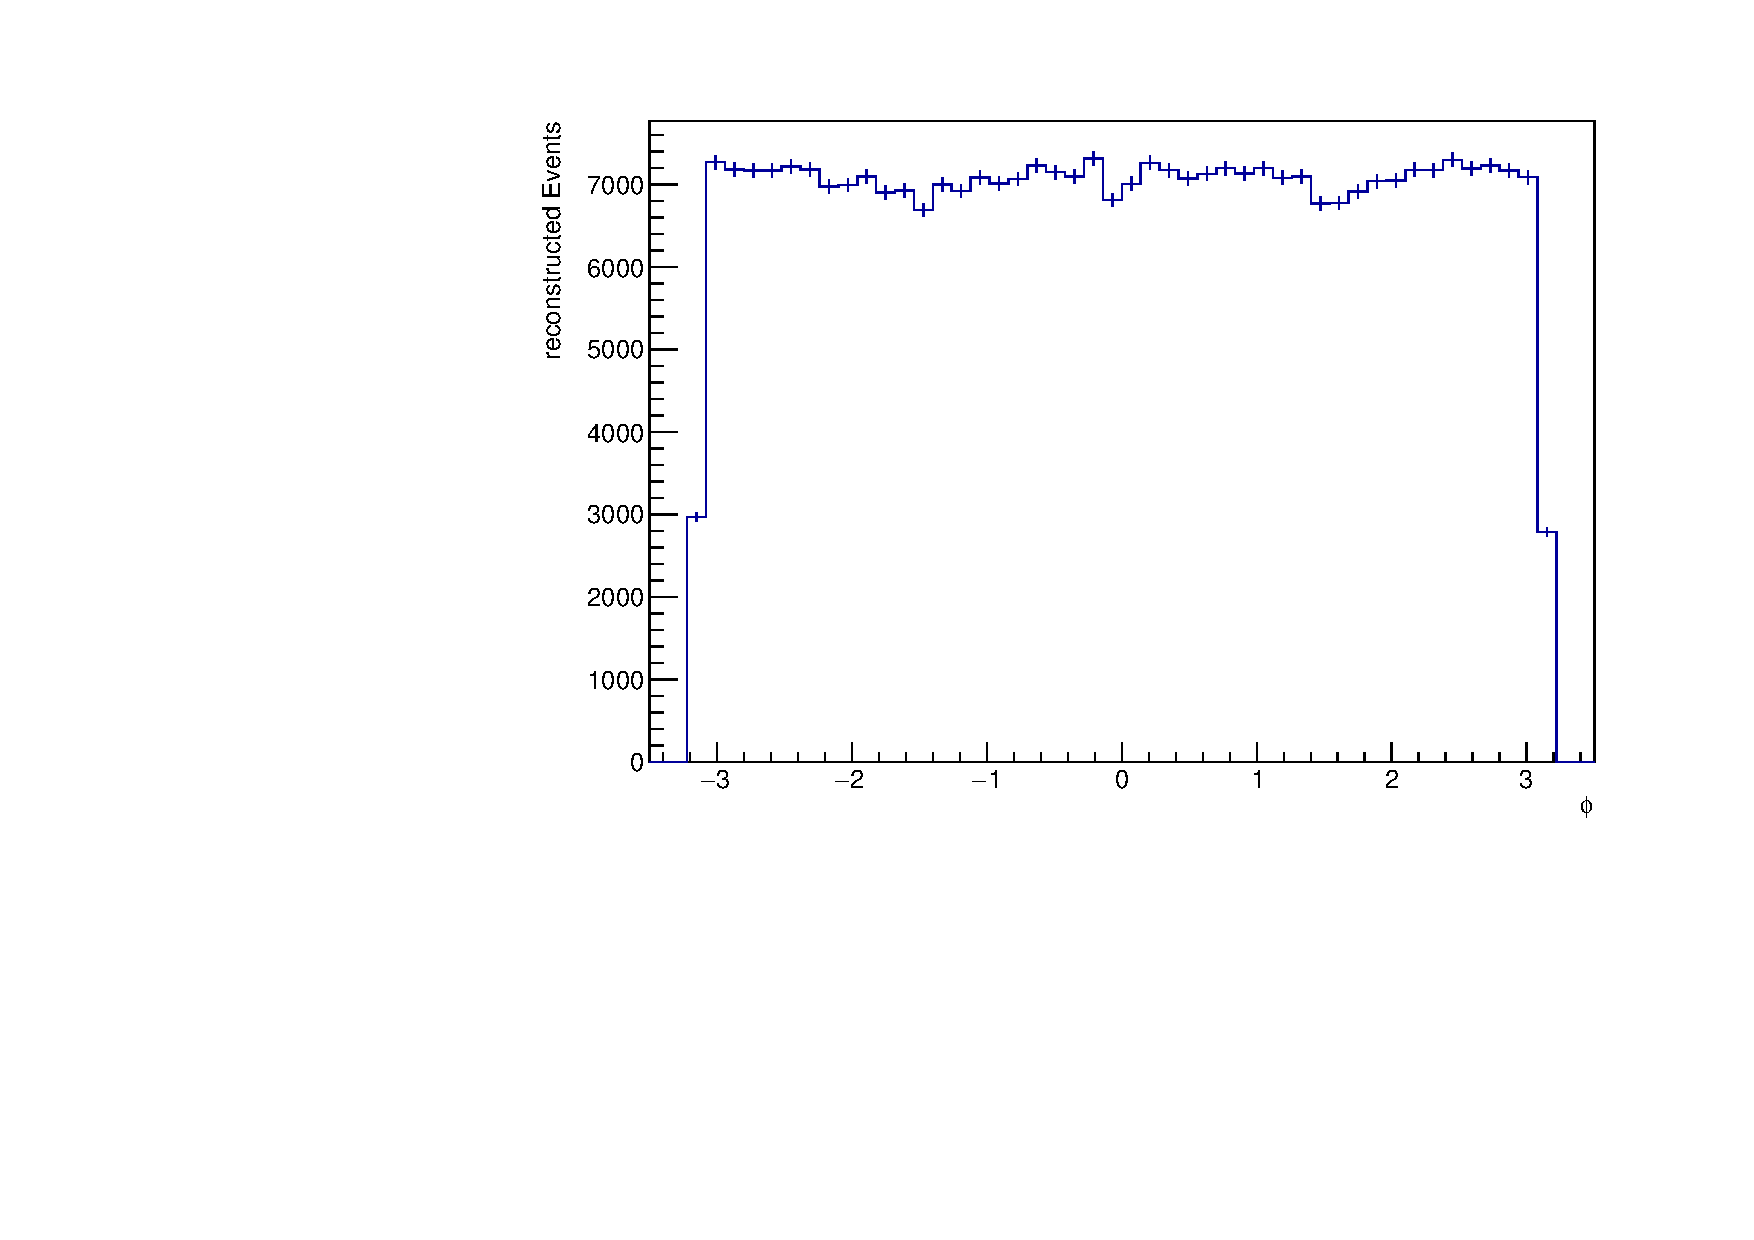
\includegraphics[width=0.9\textwidth]{up_pdf/pos/h_phi_reco_K_pos.pdf}
\end{subfigure}
\begin{subfigure}{0.45\textwidth}
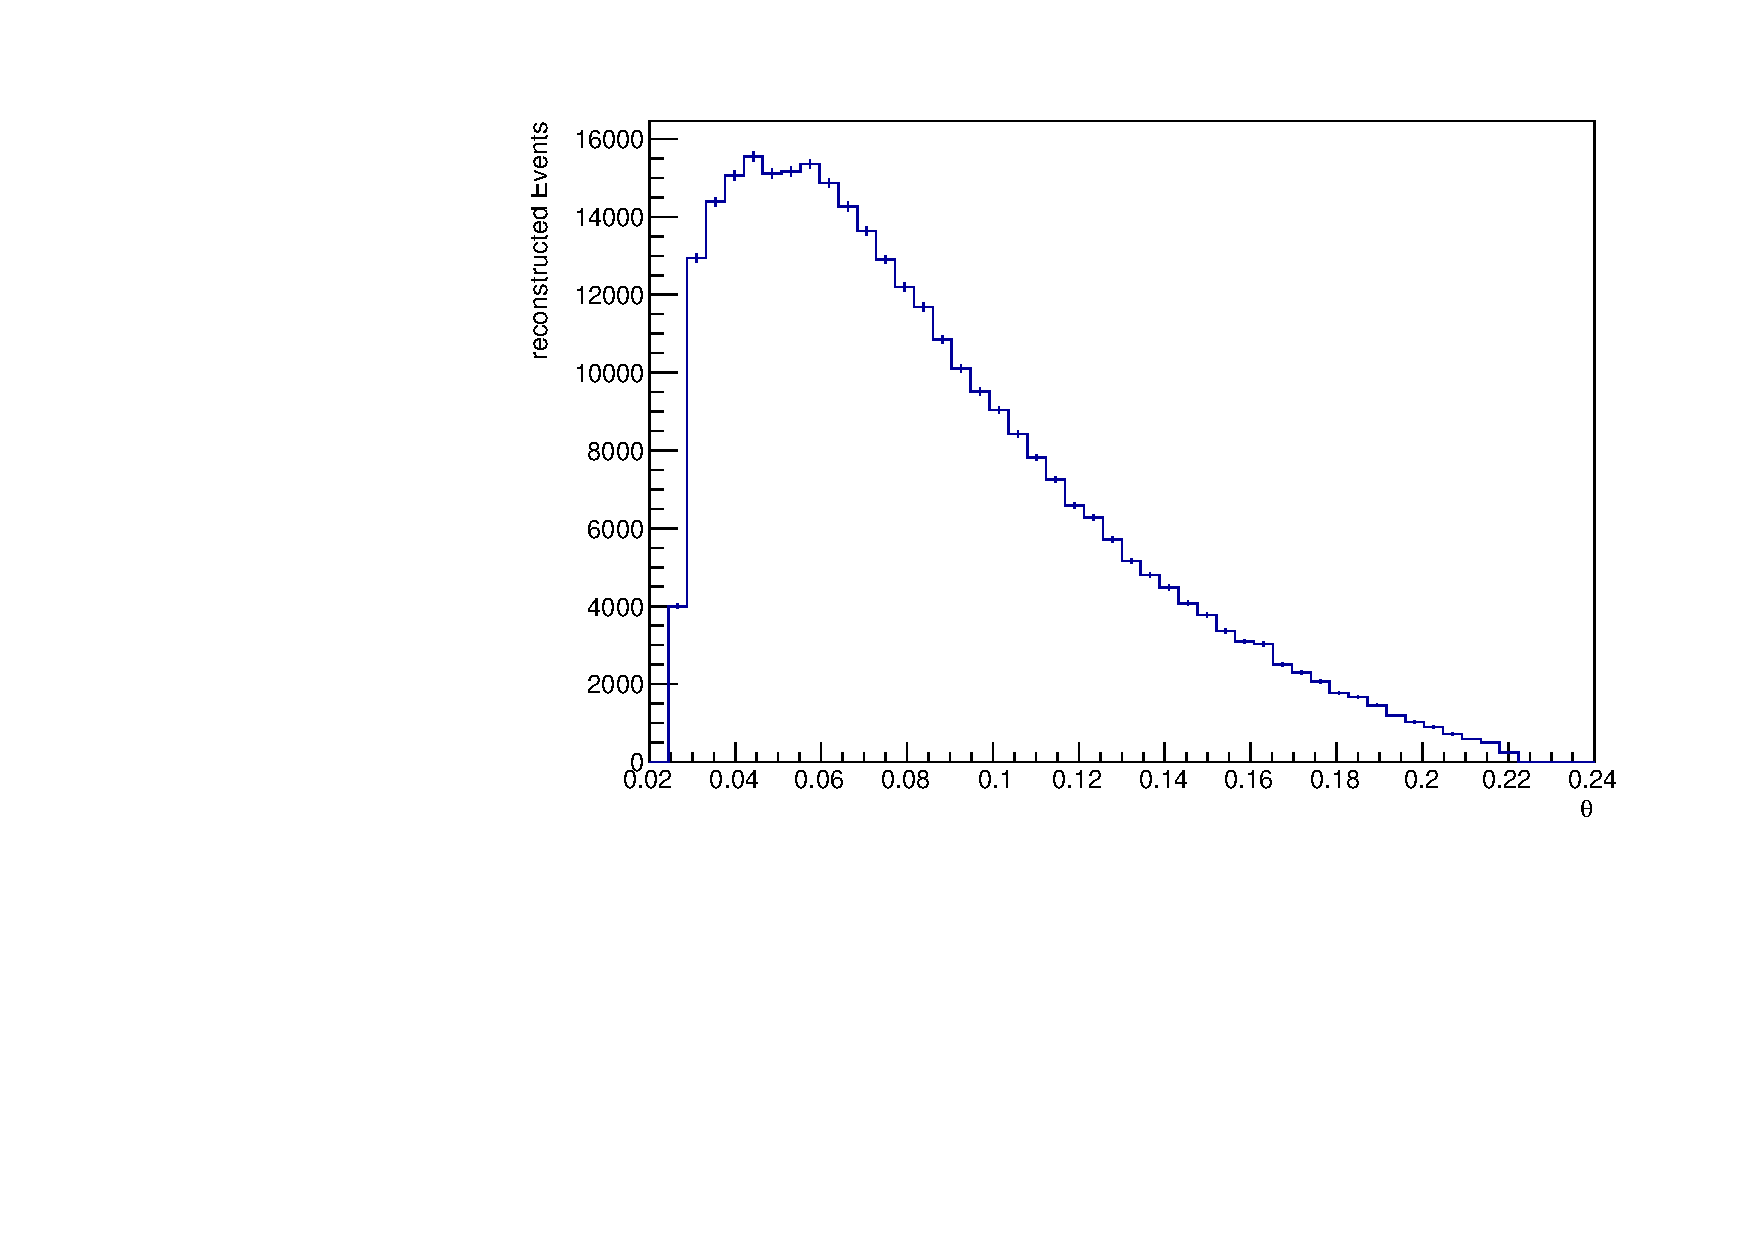
\includegraphics[width=0.9\textwidth]{up_pdf/pos/h_theta_reco_K_pos.pdf}
\end{subfigure}
\begin{subfigure}{0.45\textwidth}
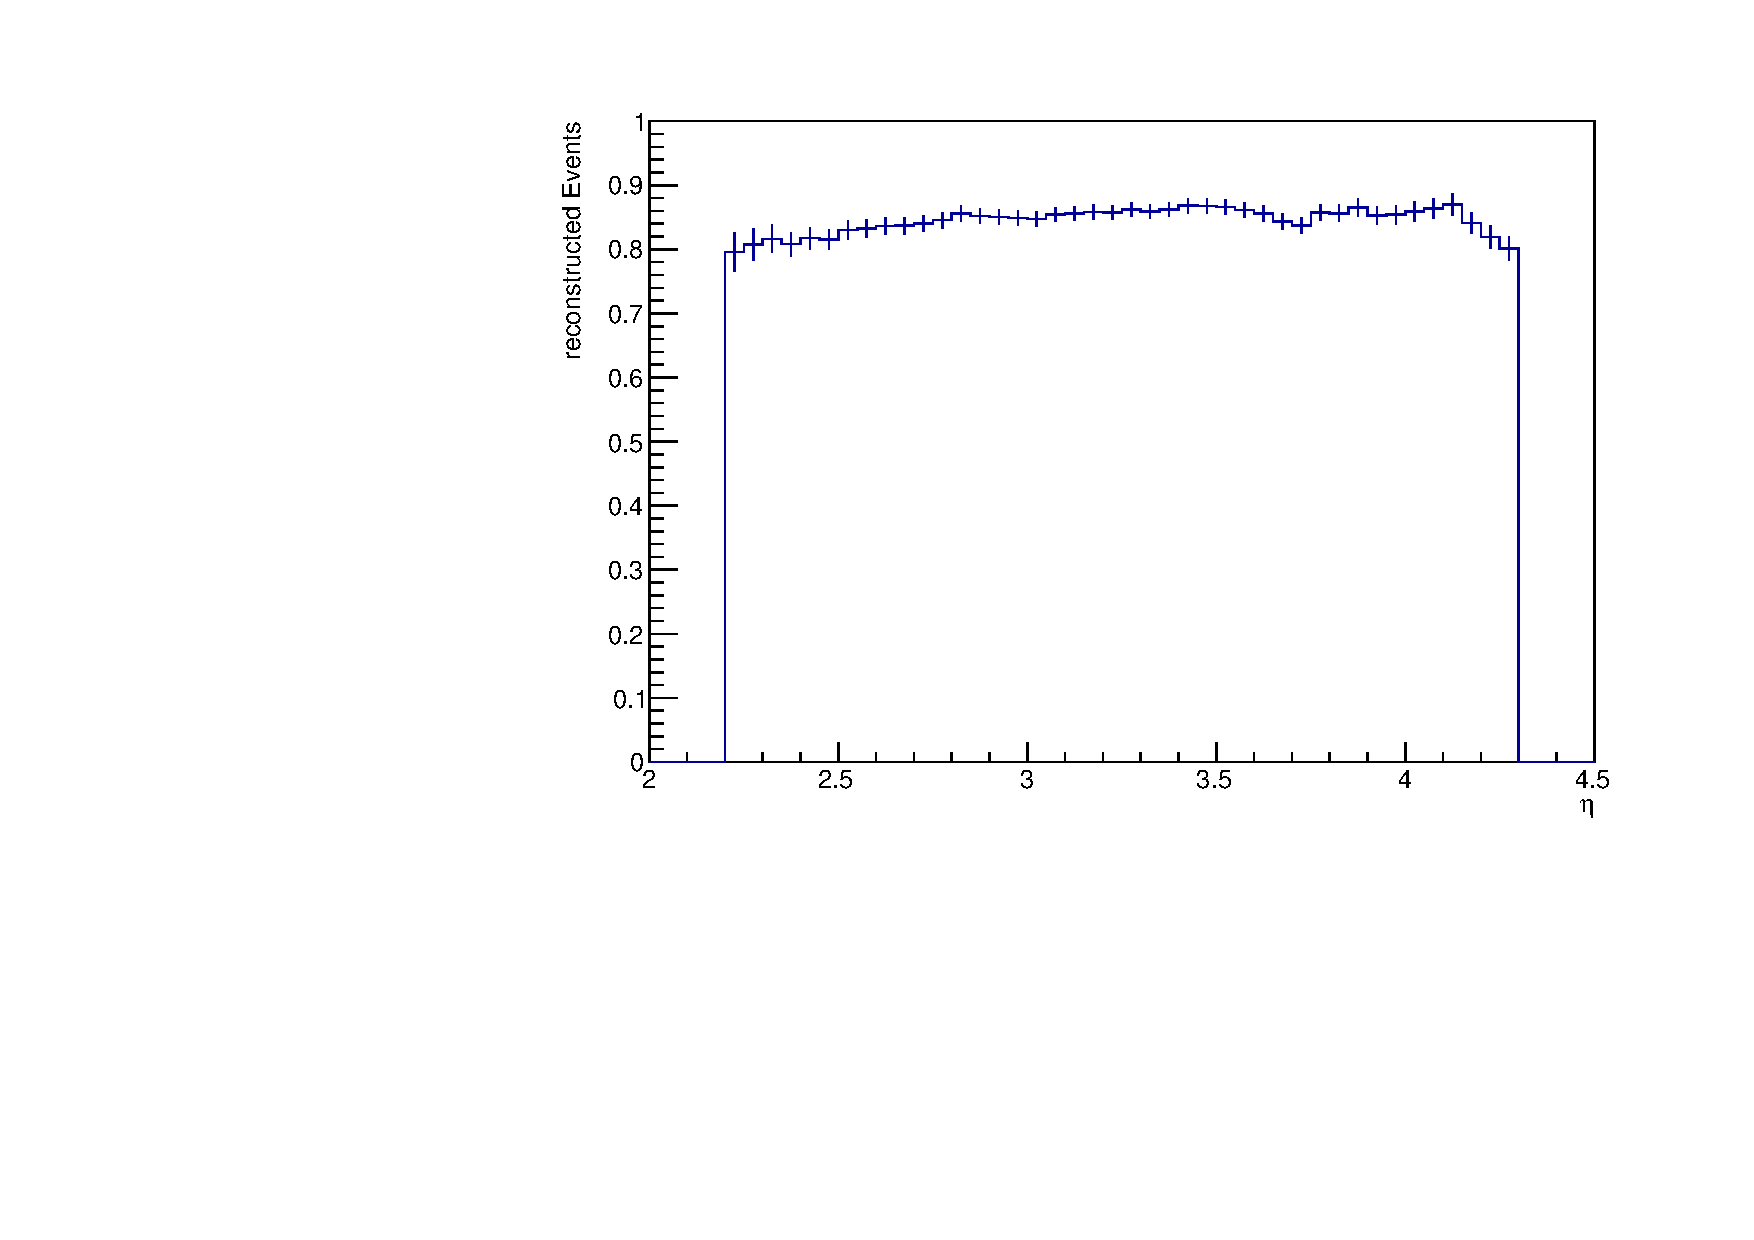
\includegraphics[width=0.9\textwidth]{up_pdf/pos/h_eta_reco_K_pos.pdf}
\end{subfigure}
\end{figure}
\end{frame}
\begin{frame}{soft $\pi$-efficiency}
\begin{figure}
\begin{subfigure}{0.45\textwidth}
\includegraphics[width=0.9\textwidth]{up_pdf/pos/h_pt_reco_SPi_pos.pdf}
\end{subfigure}
\begin{subfigure}{0.45\textwidth}
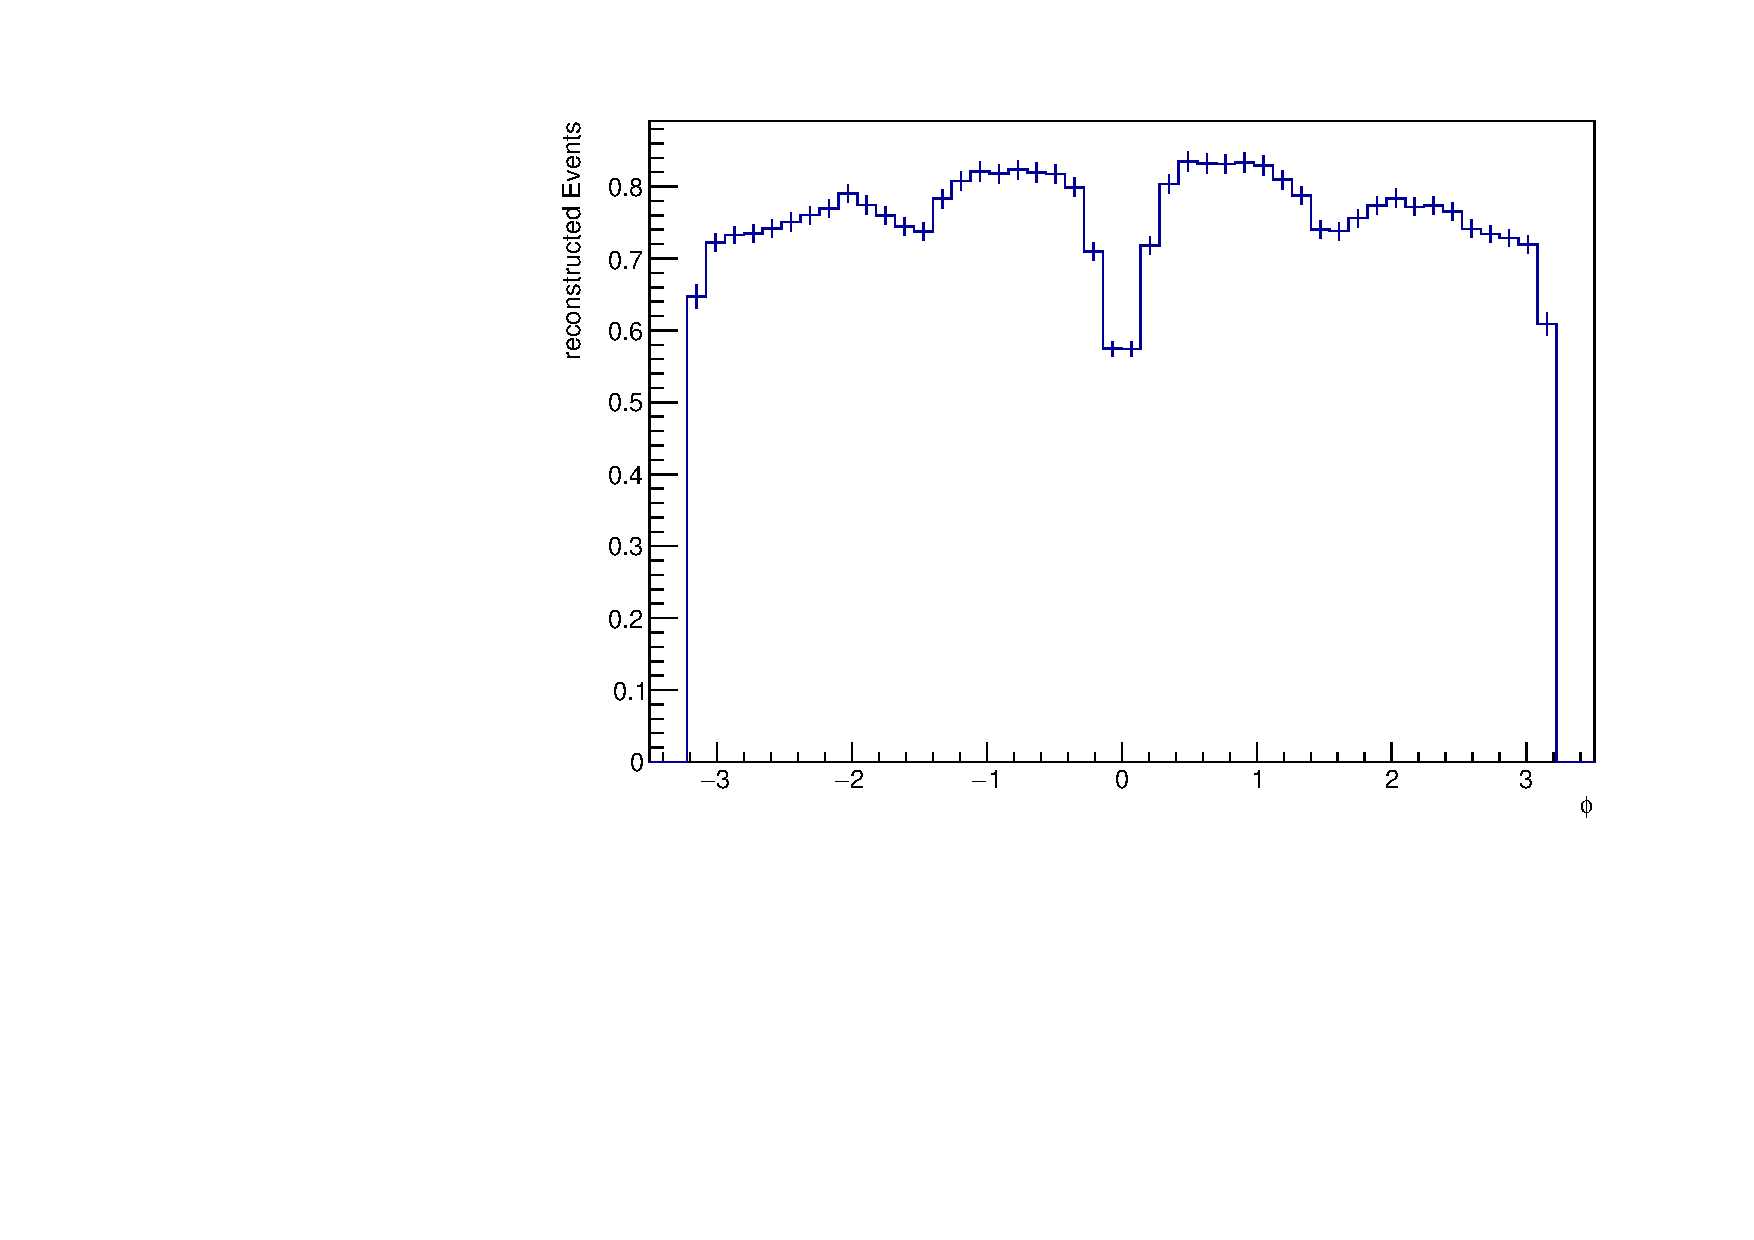
\includegraphics[width=0.9\textwidth]{up_pdf/pos/h_phi_reco_SPi_pos.pdf}
\end{subfigure}
\begin{subfigure}{0.45\textwidth}
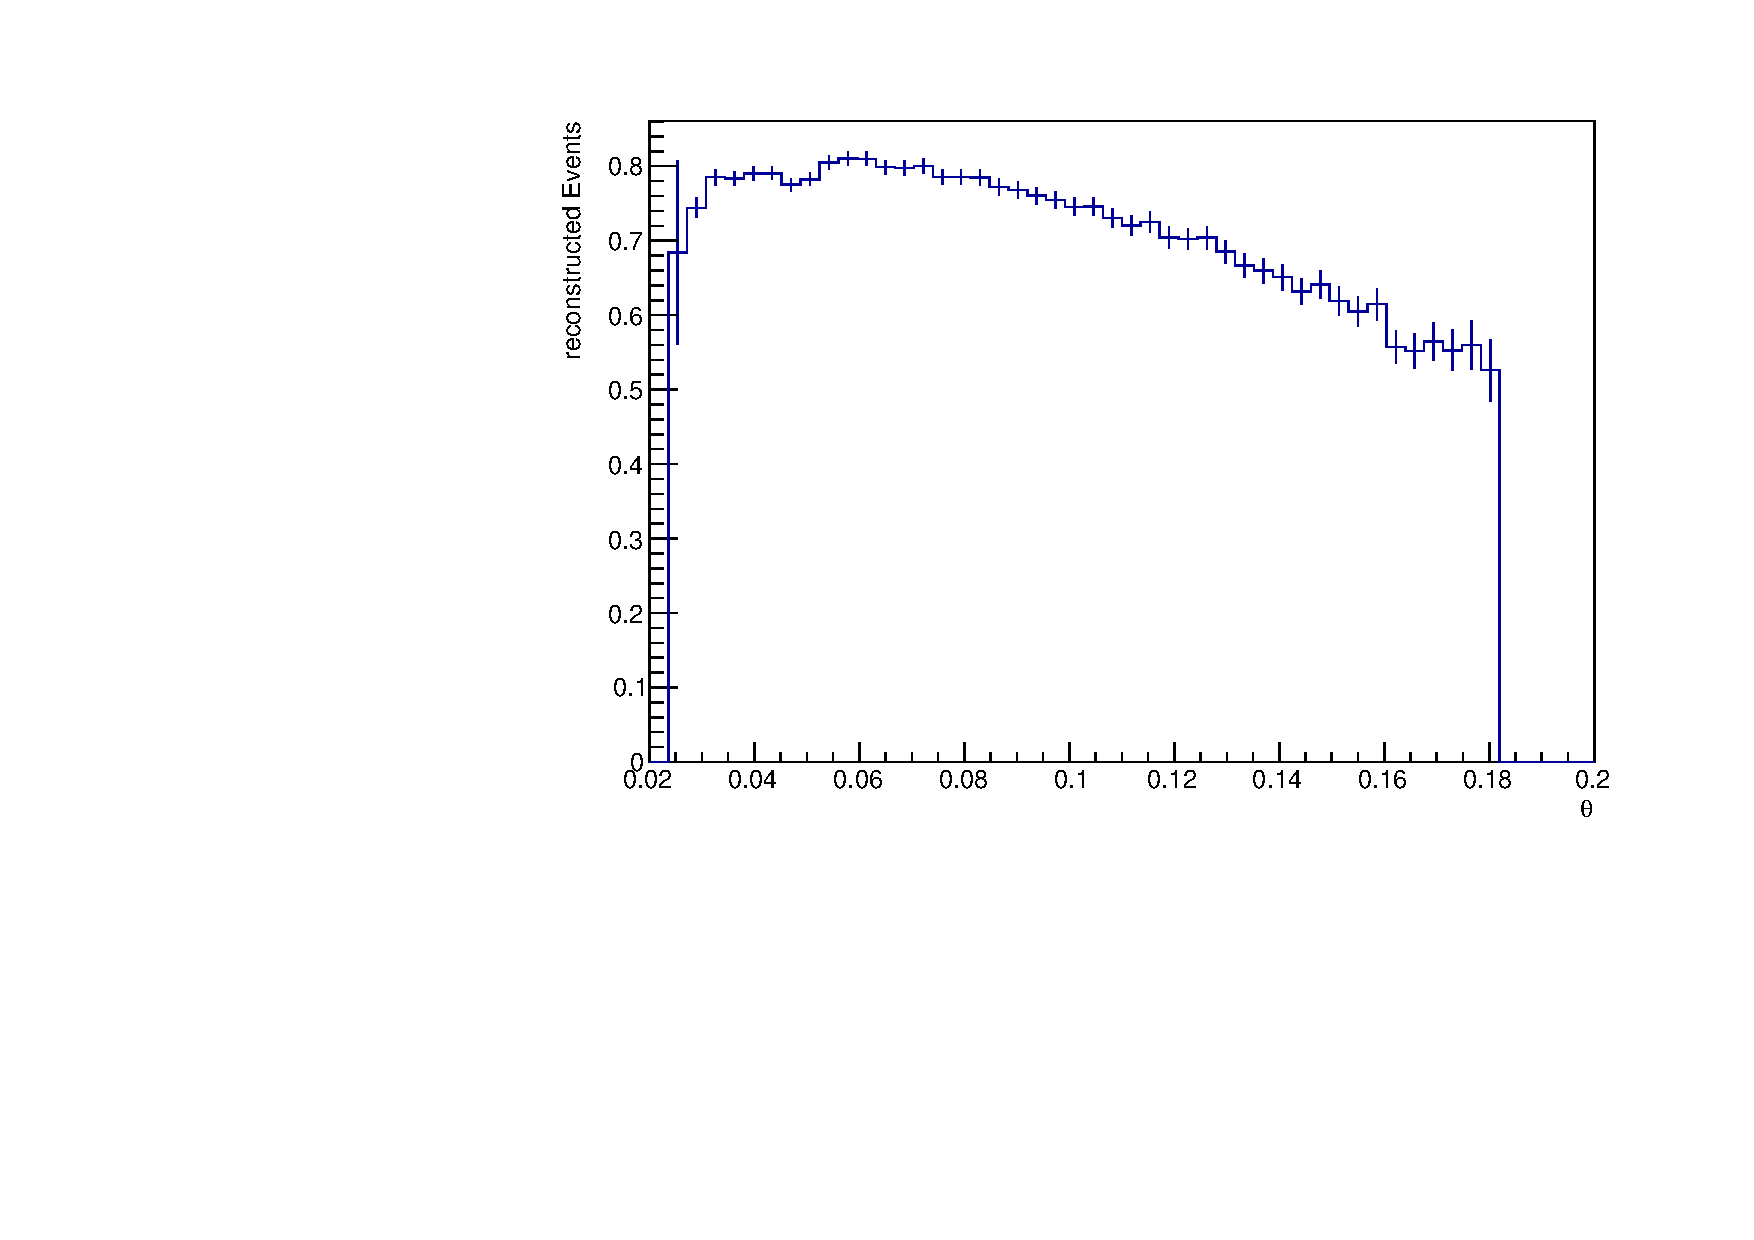
\includegraphics[width=0.9\textwidth]{up_pdf/pos/h_theta_reco_SPi_pos.pdf}
\end{subfigure}
\begin{subfigure}{0.45\textwidth}
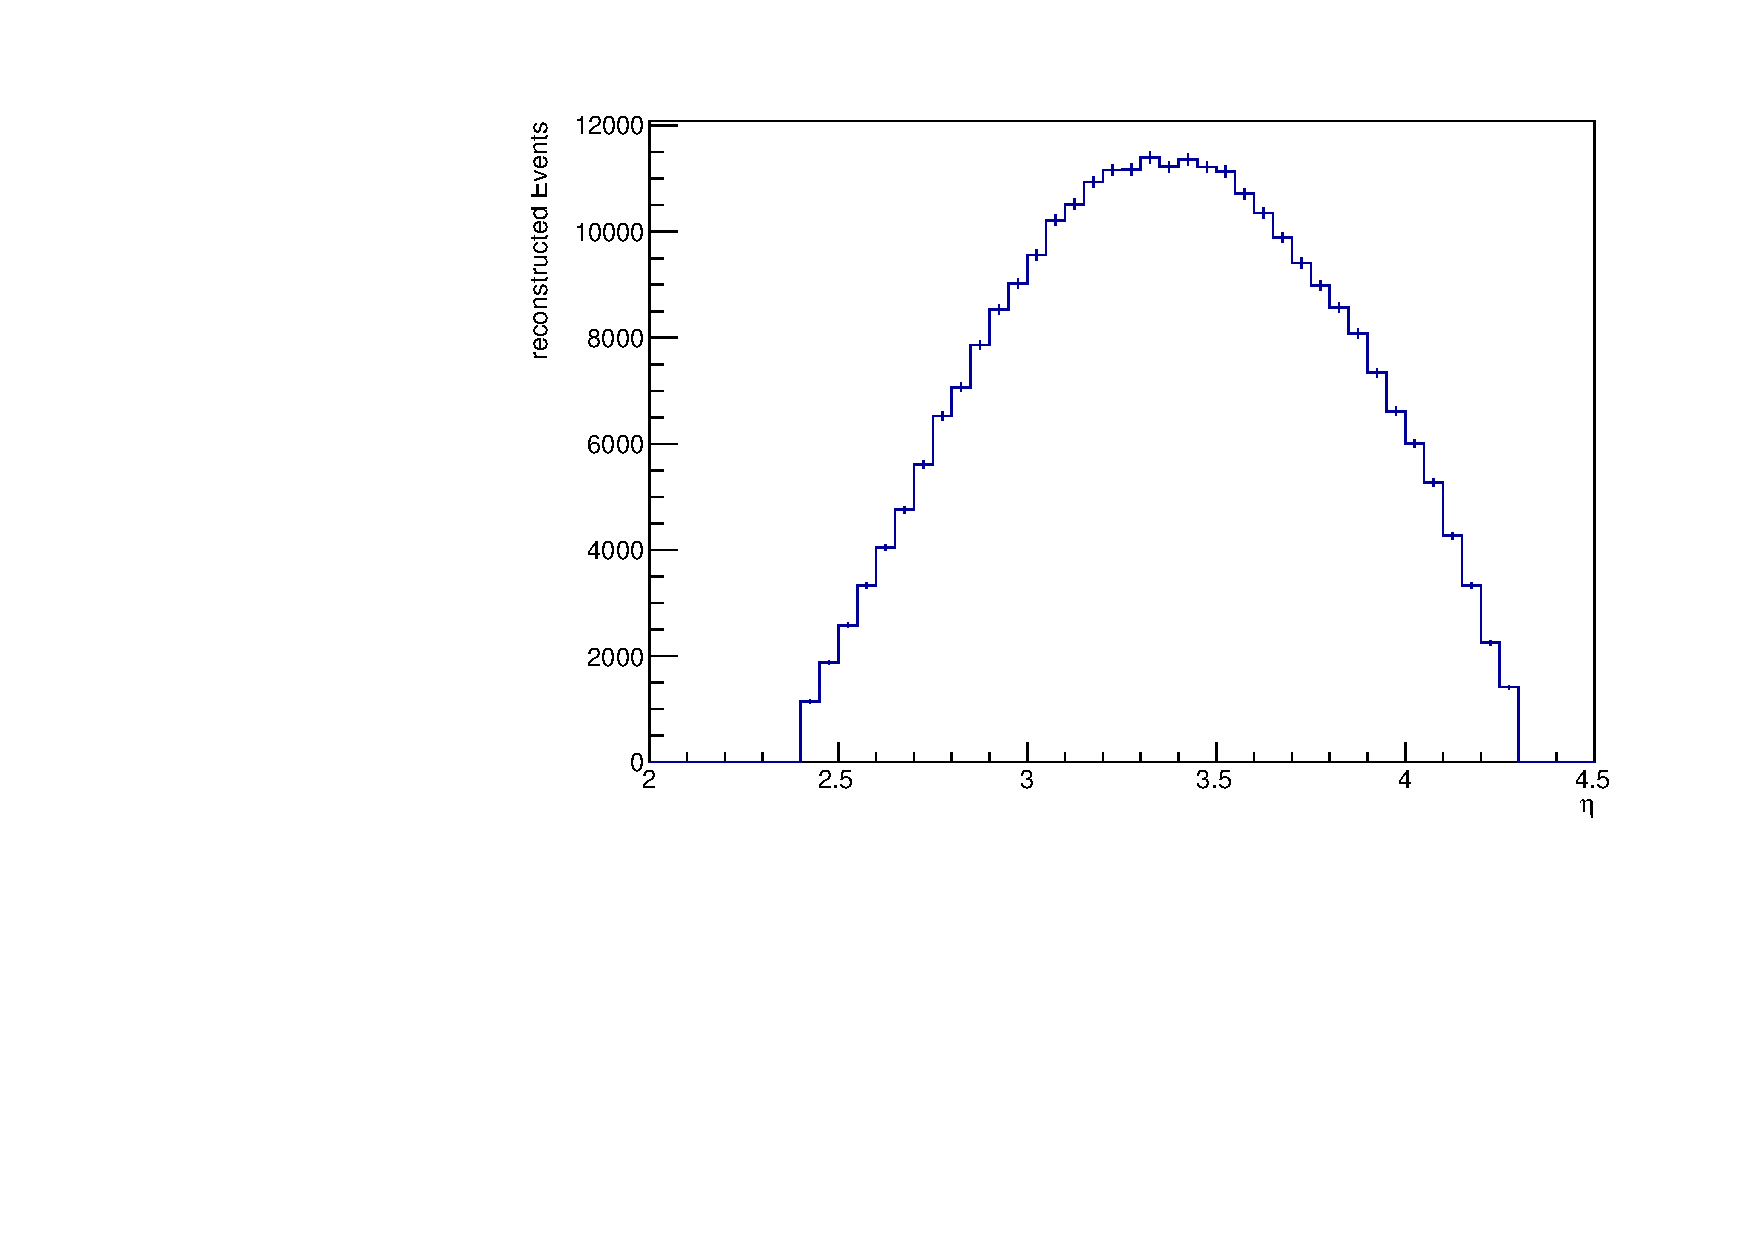
\includegraphics[width=0.9\textwidth]{up_pdf/pos/h_eta_reco_SPi_pos.pdf}
\end{subfigure}
\end{figure}
\end{frame}
\begin{frame}{$D^0$-efficiency}
\begin{figure}
\begin{subfigure}{0.45\textwidth}
\includegraphics[width=0.9\textwidth]{up_pdf/pos/h_pt_reco_D0_pos.pdf}
\end{subfigure}
\begin{subfigure}{0.45\textwidth}
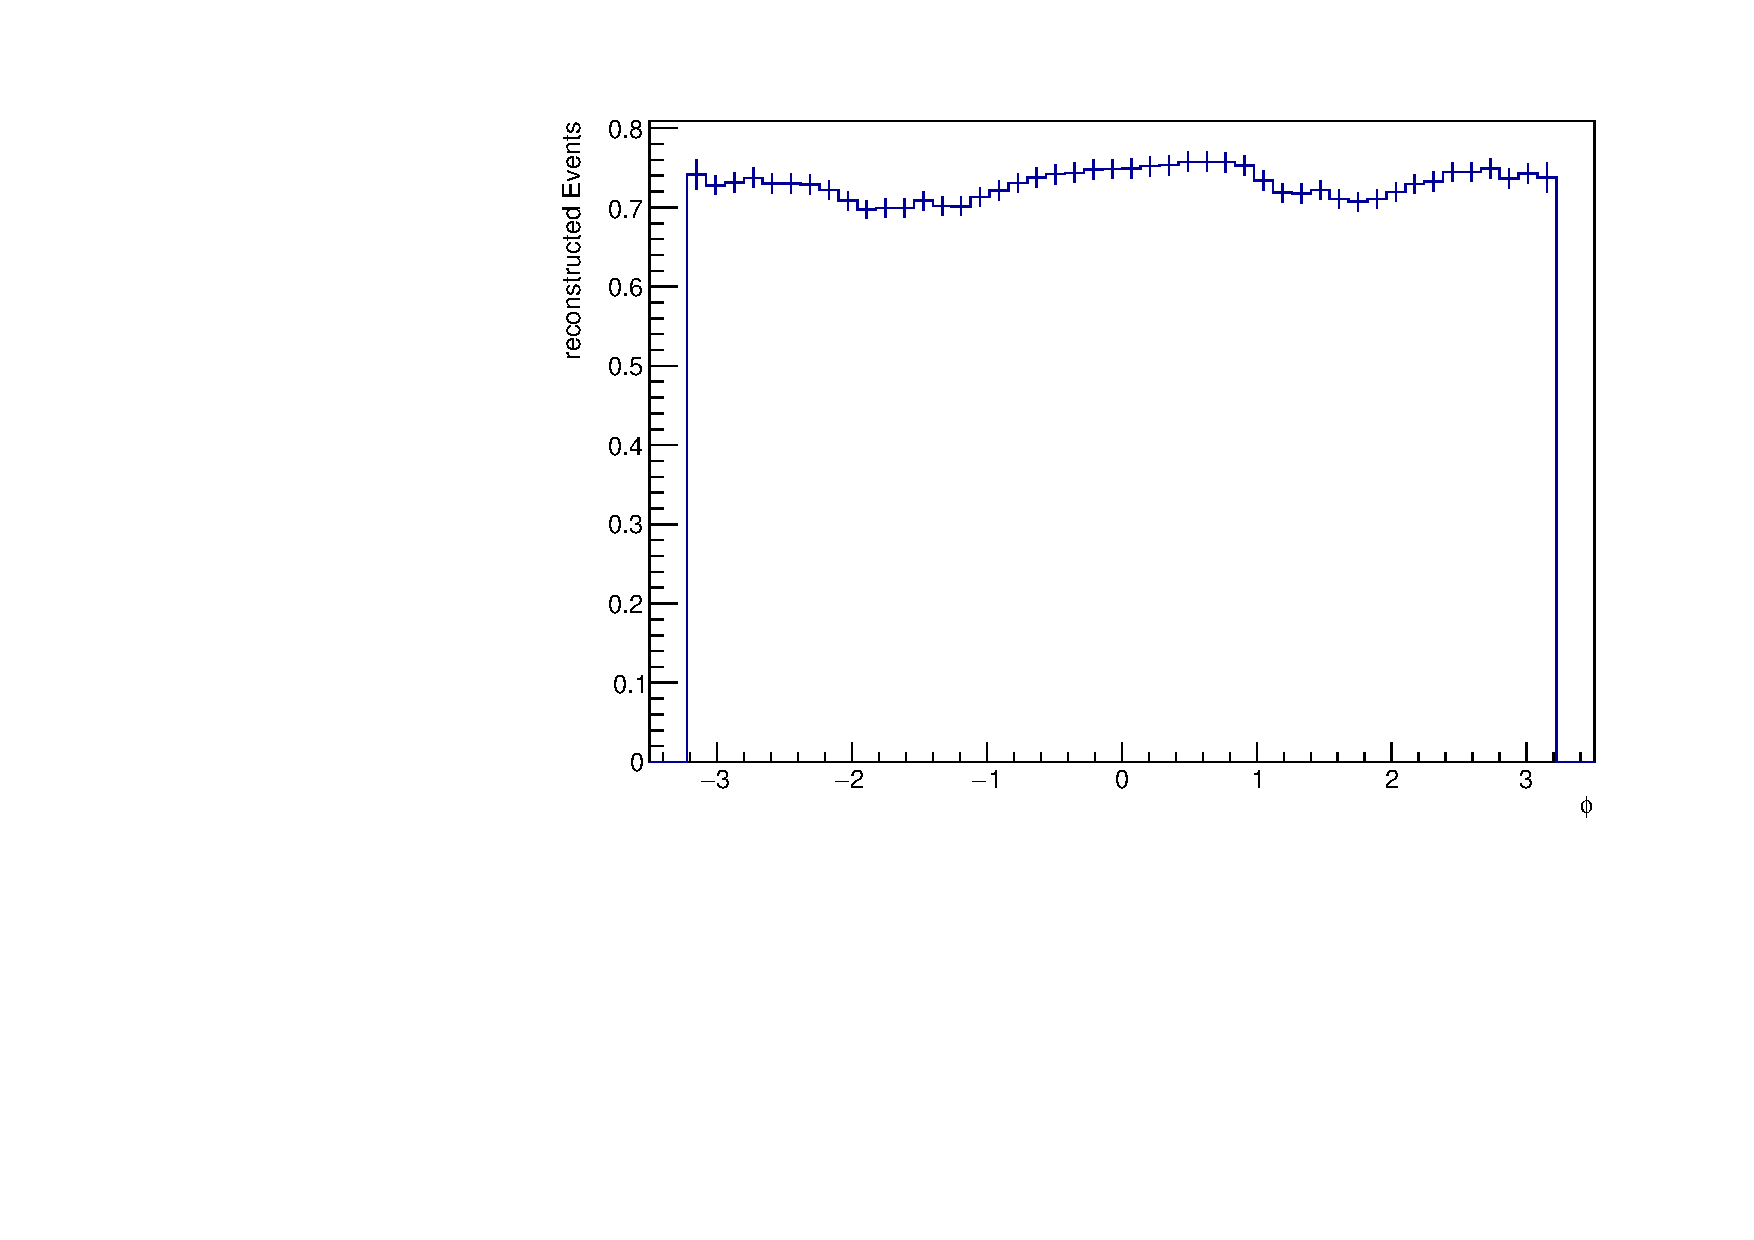
\includegraphics[width=0.9\textwidth]{up_pdf/pos/h_phi_reco_D0_pos.pdf}
\end{subfigure}
\begin{subfigure}{0.45\textwidth}
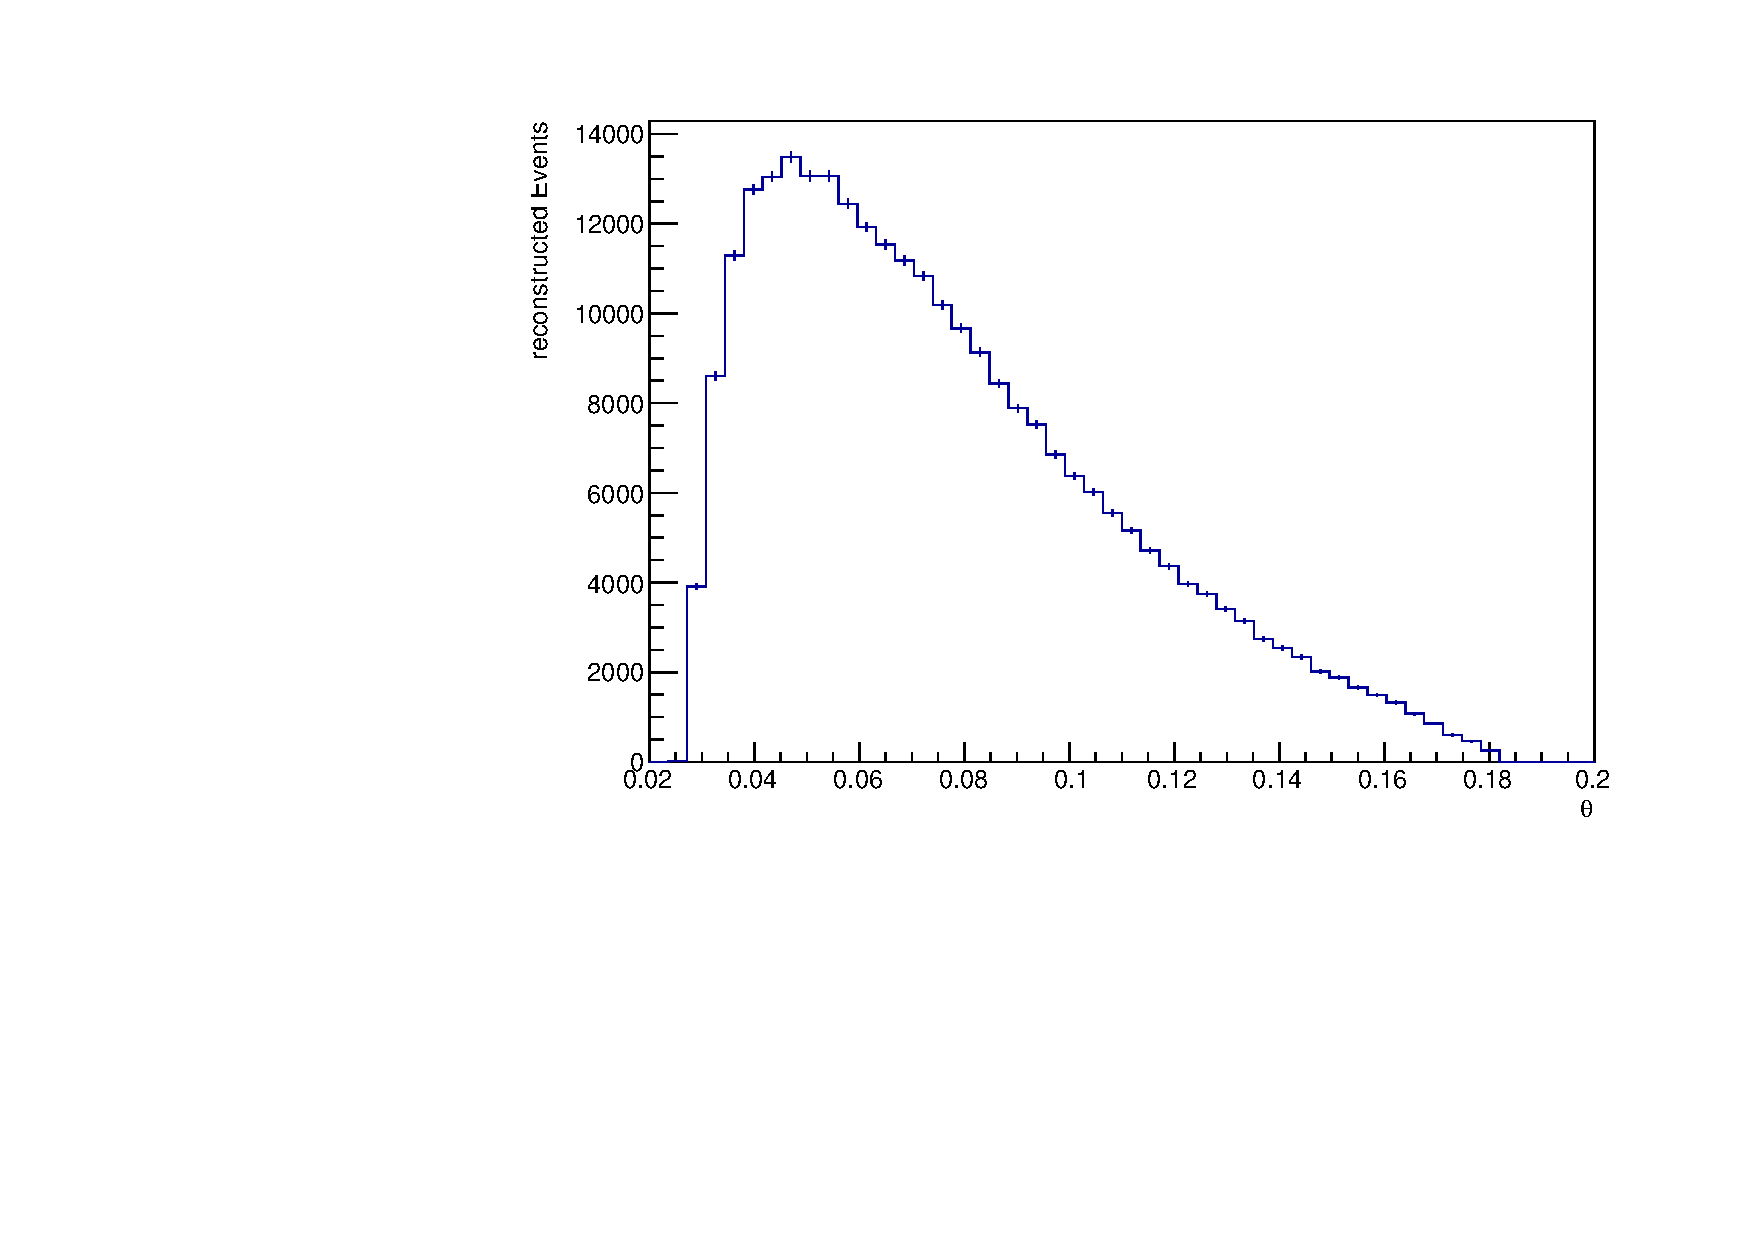
\includegraphics[width=0.9\textwidth]{up_pdf/pos/h_theta_reco_D0_pos.pdf}
\end{subfigure}
\begin{subfigure}{0.45\textwidth}
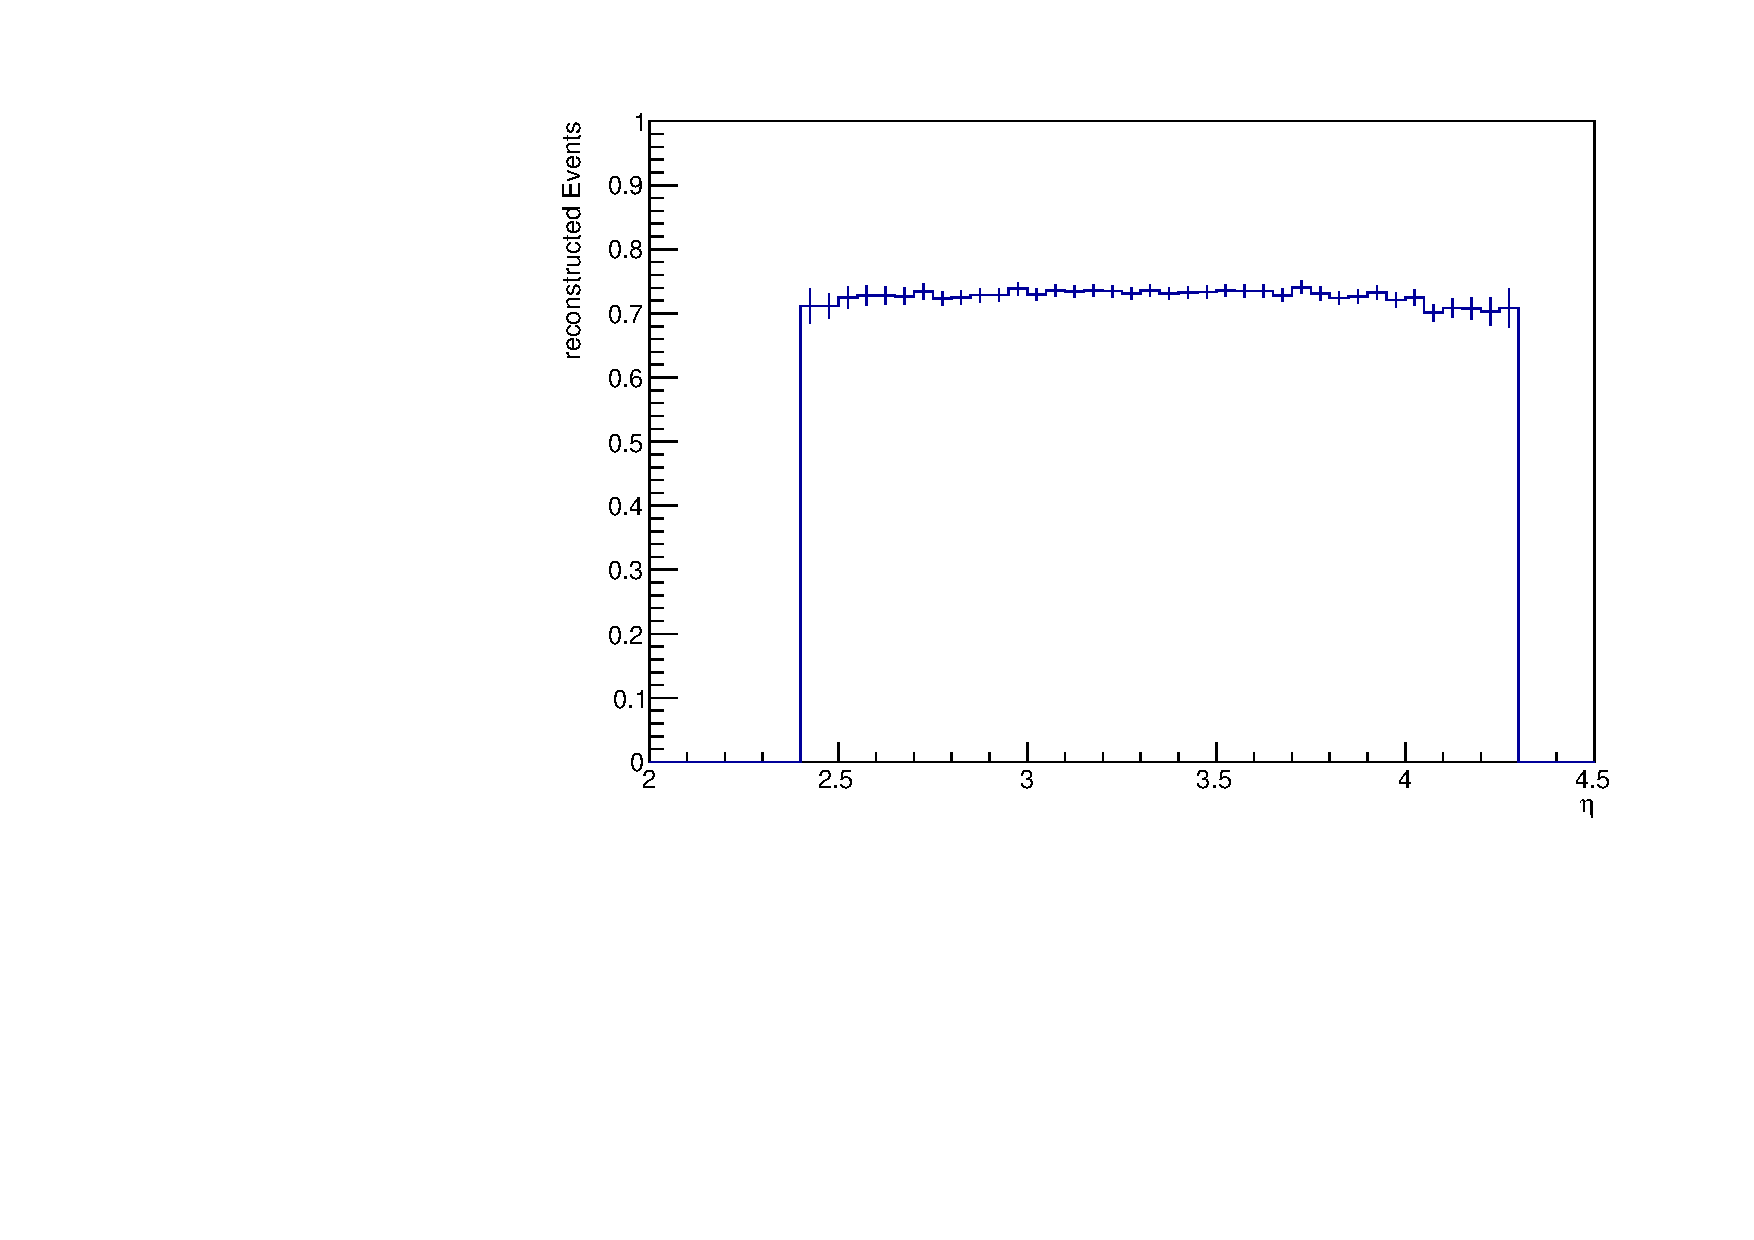
\includegraphics[width=0.9\textwidth]{up_pdf/pos/h_eta_reco_D0_pos.pdf}
\end{subfigure}
\end{figure}
\end{frame}
\begin{frame}{$D^*$-efficiency}
\begin{figure}
\begin{subfigure}{0.45\textwidth}
\includegraphics[width=0.9\textwidth]{up_pdf/pos/h_pt_reco_Dst_pos.pdf}
\end{subfigure}
\begin{subfigure}{0.45\textwidth}
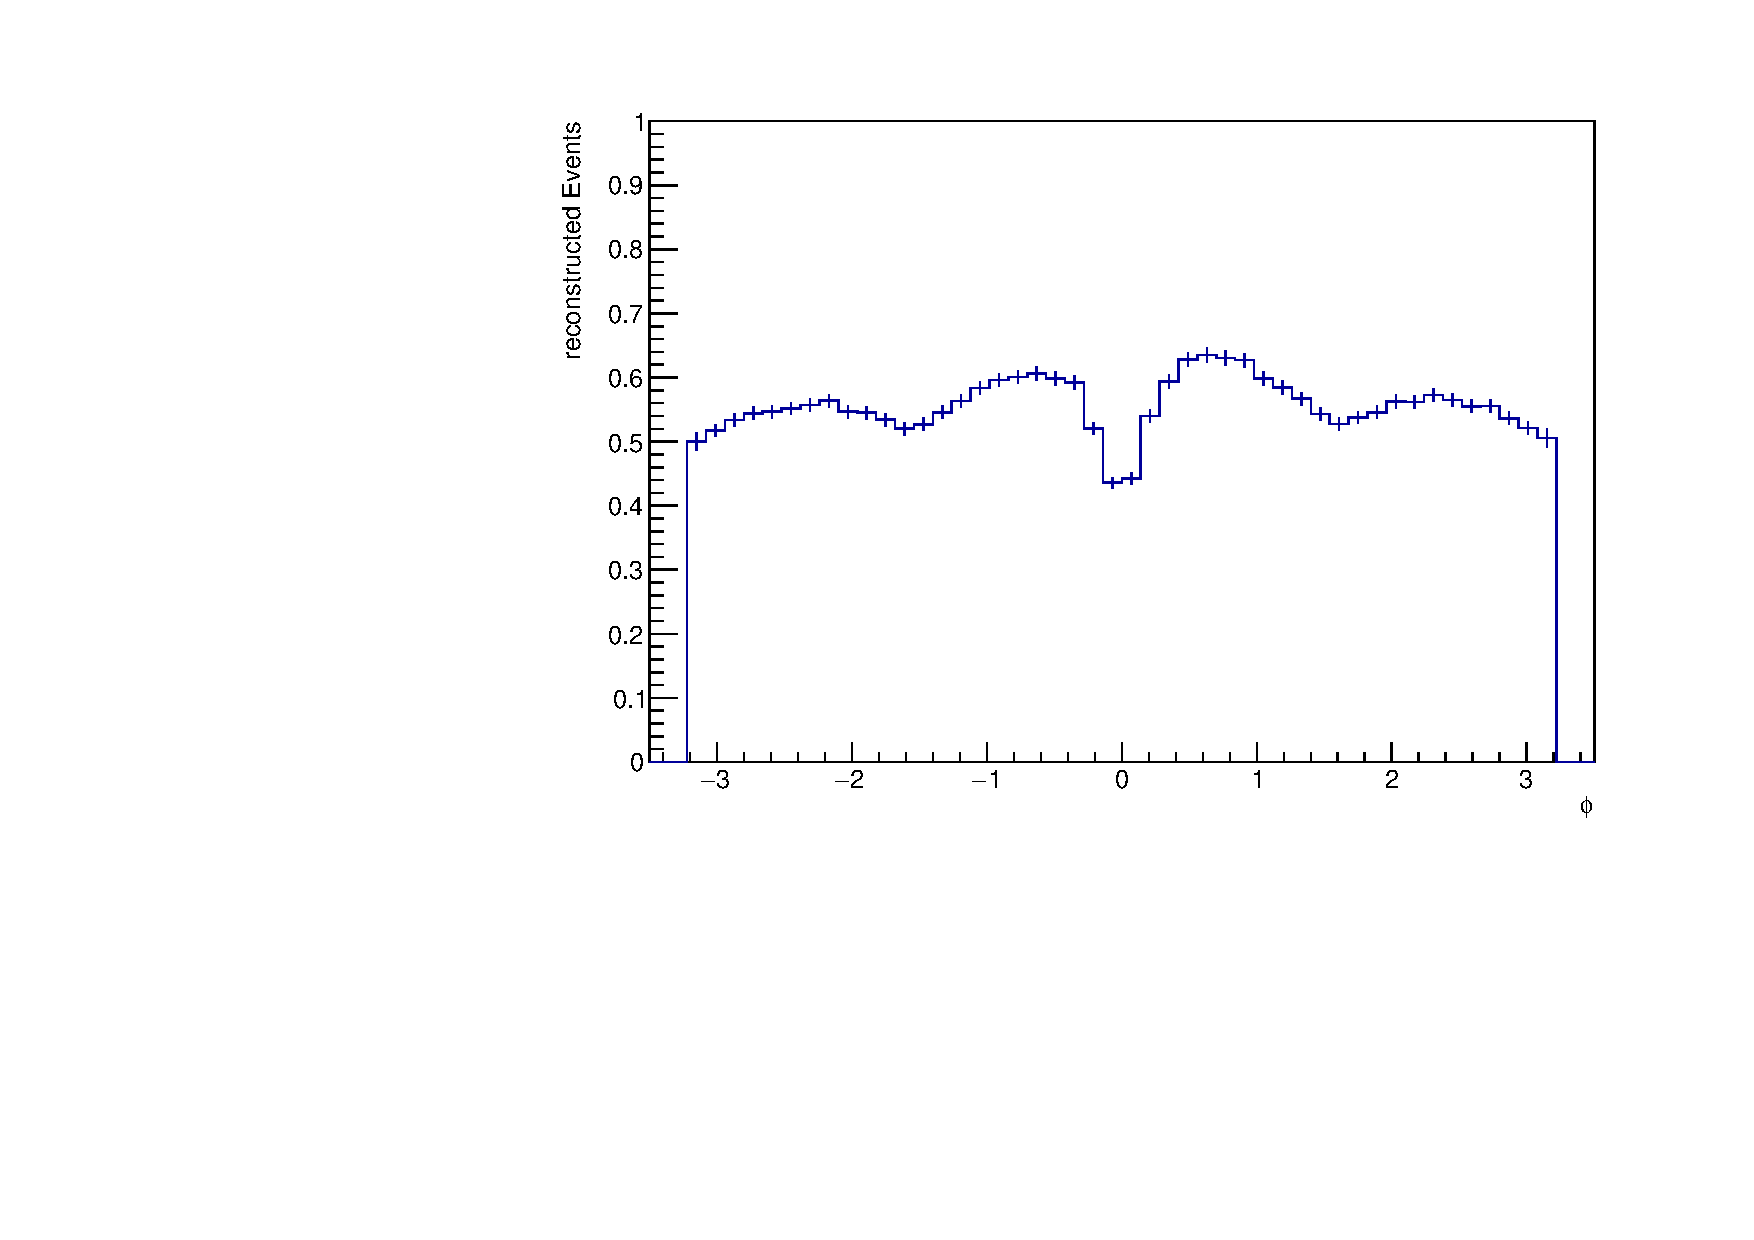
\includegraphics[width=0.9\textwidth]{up_pdf/pos/h_phi_reco_Dst_pos.pdf}
\end{subfigure}
\begin{subfigure}{0.45\textwidth}
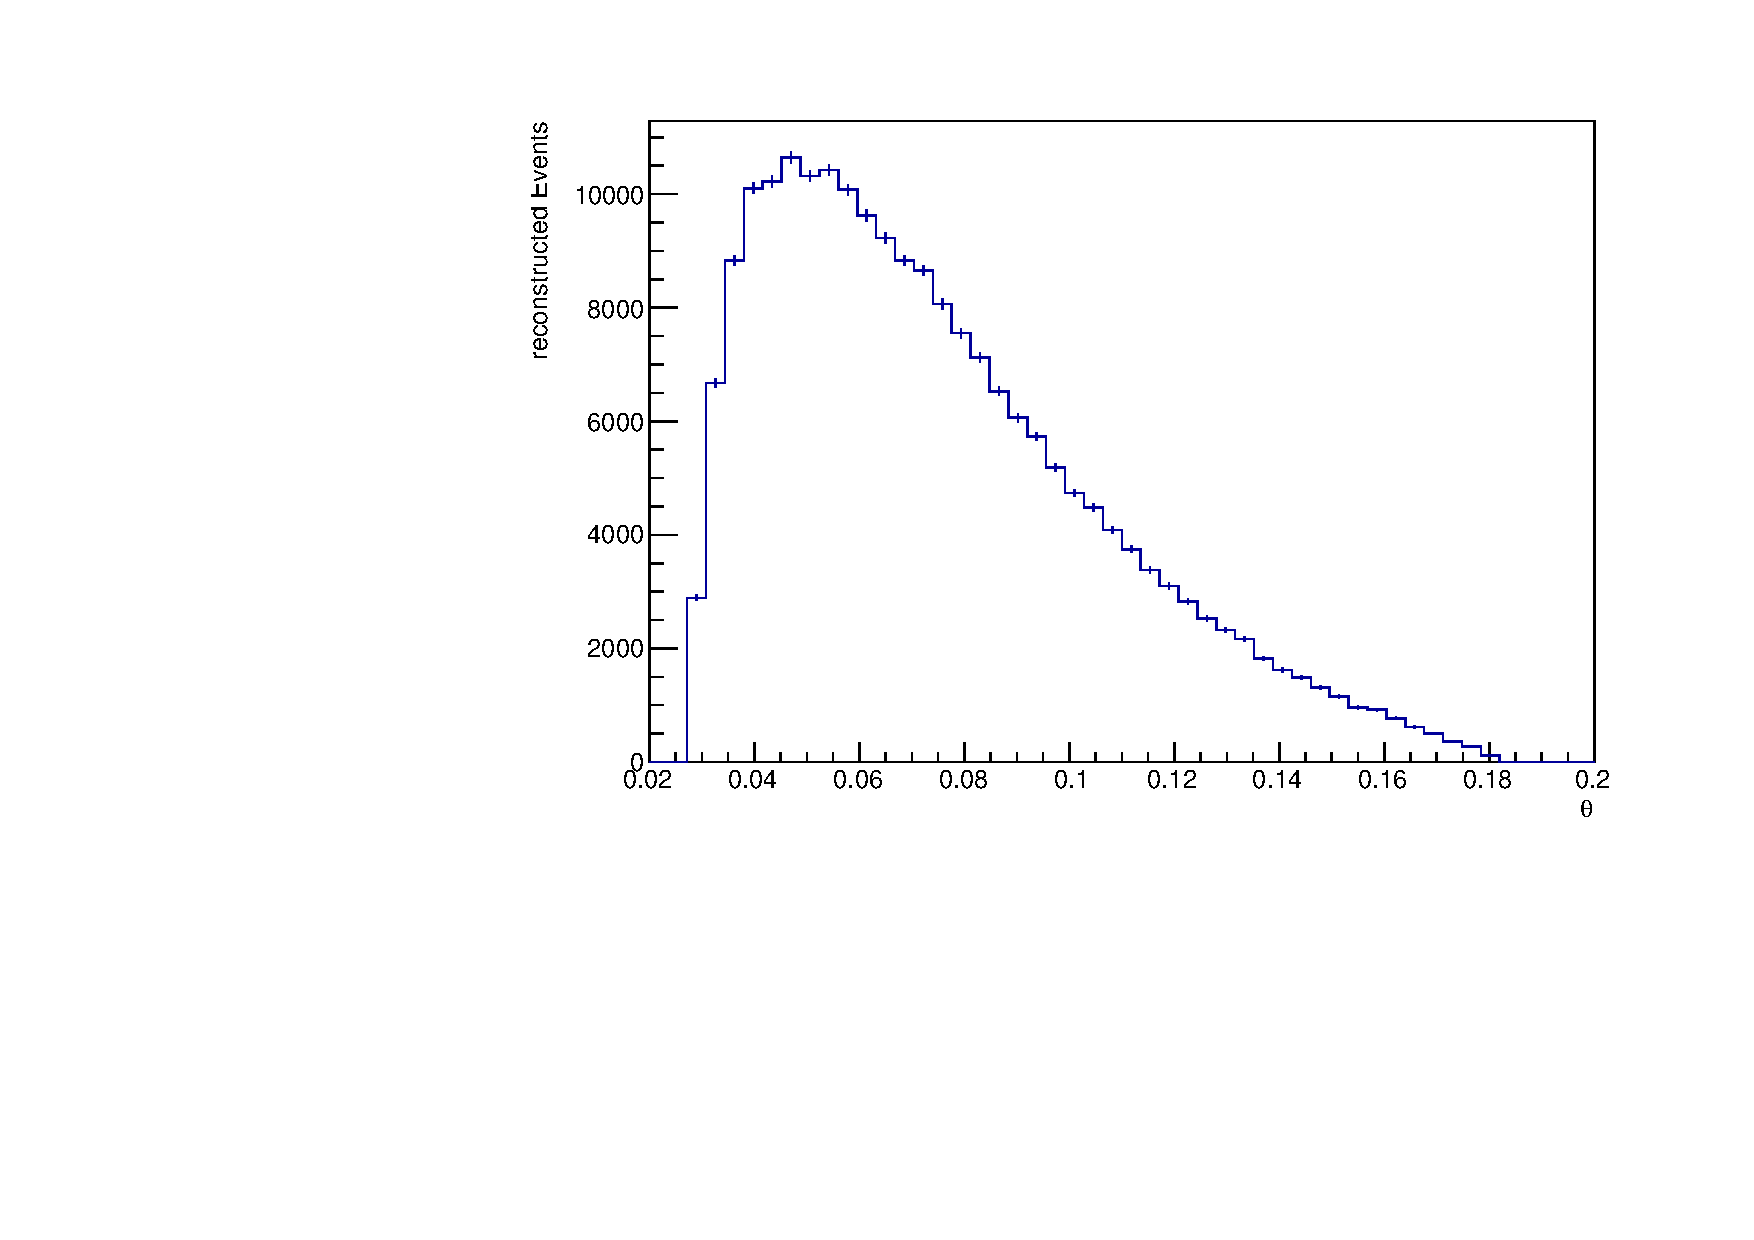
\includegraphics[width=0.9\textwidth]{up_pdf/pos/h_theta_reco_Dst_pos.pdf}
\end{subfigure}
\begin{subfigure}{0.45\textwidth}
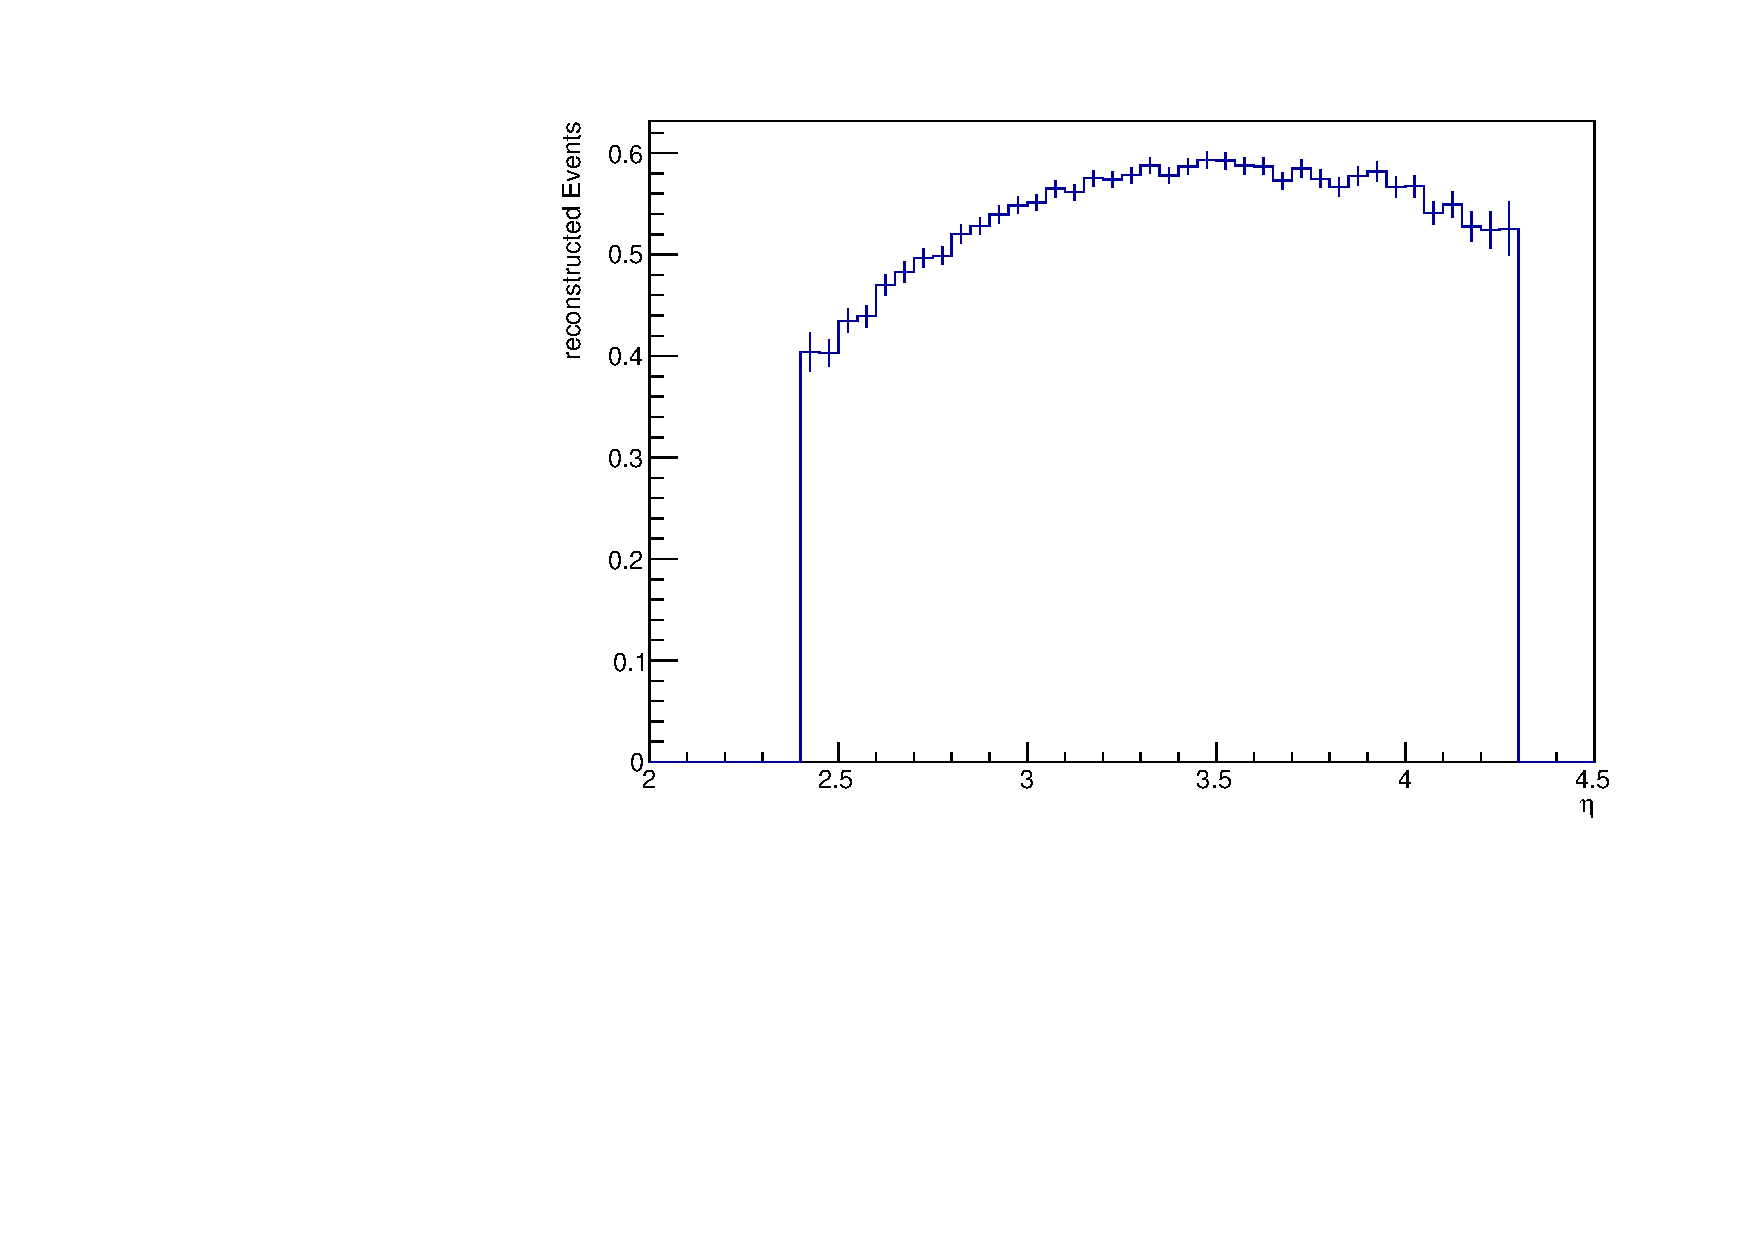
\includegraphics[width=0.9\textwidth]{up_pdf/pos/h_eta_reco_Dst_pos.pdf}
\end{subfigure}
\end{figure}
\end{frame}
\begin{frame}
\begin{LARGE}
\textbf{Charge: -}
\end{LARGE}
\end{frame}
\begin{frame}{$\pi$-efficiency}
\begin{figure}
\begin{subfigure}{0.45\textwidth}
\includegraphics[width=0.9\textwidth]{up_pdf/neg/h_pt_reco_Pi_neg.pdf}
\end{subfigure}
\begin{subfigure}{0.45\textwidth}
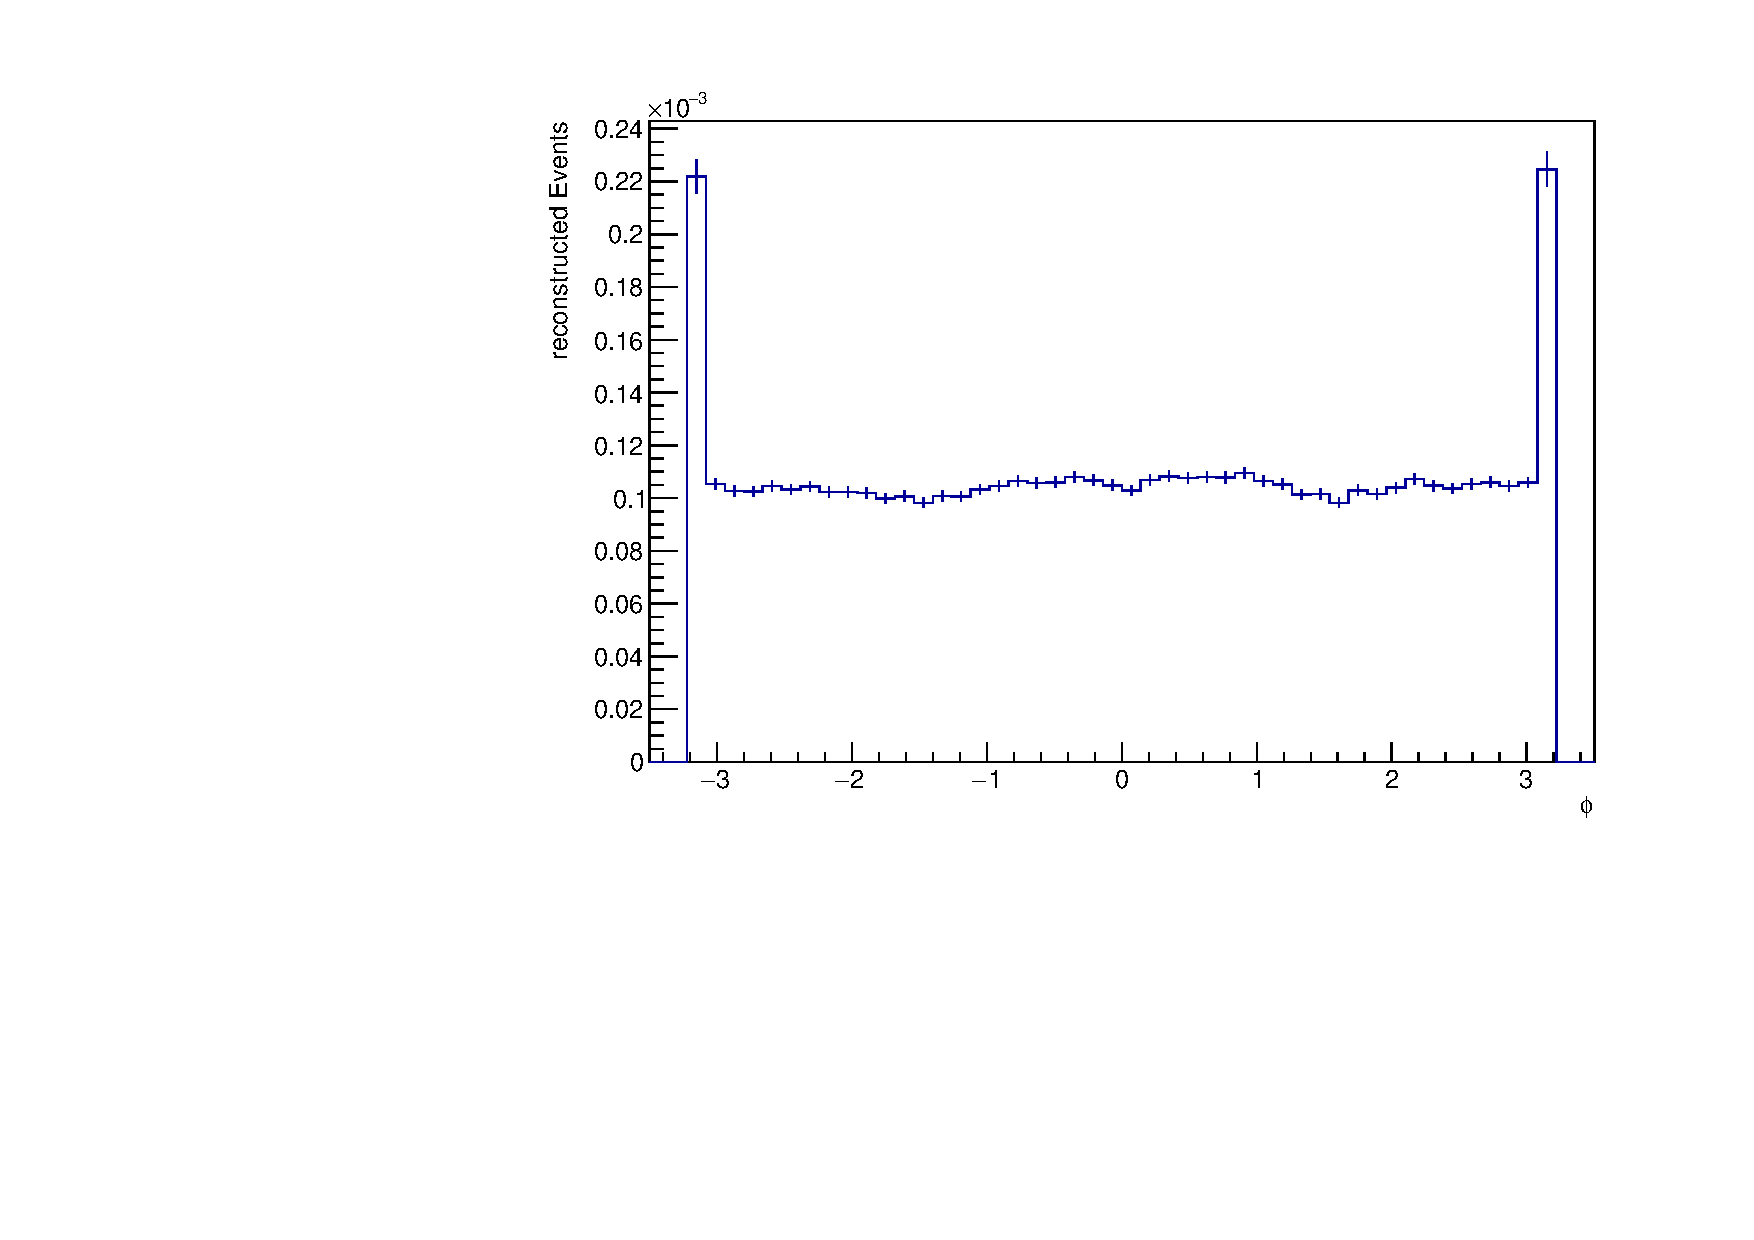
\includegraphics[width=0.9\textwidth]{up_pdf/neg/h_phi_reco_Pi_neg.pdf}
\end{subfigure}
\begin{subfigure}{0.45\textwidth}
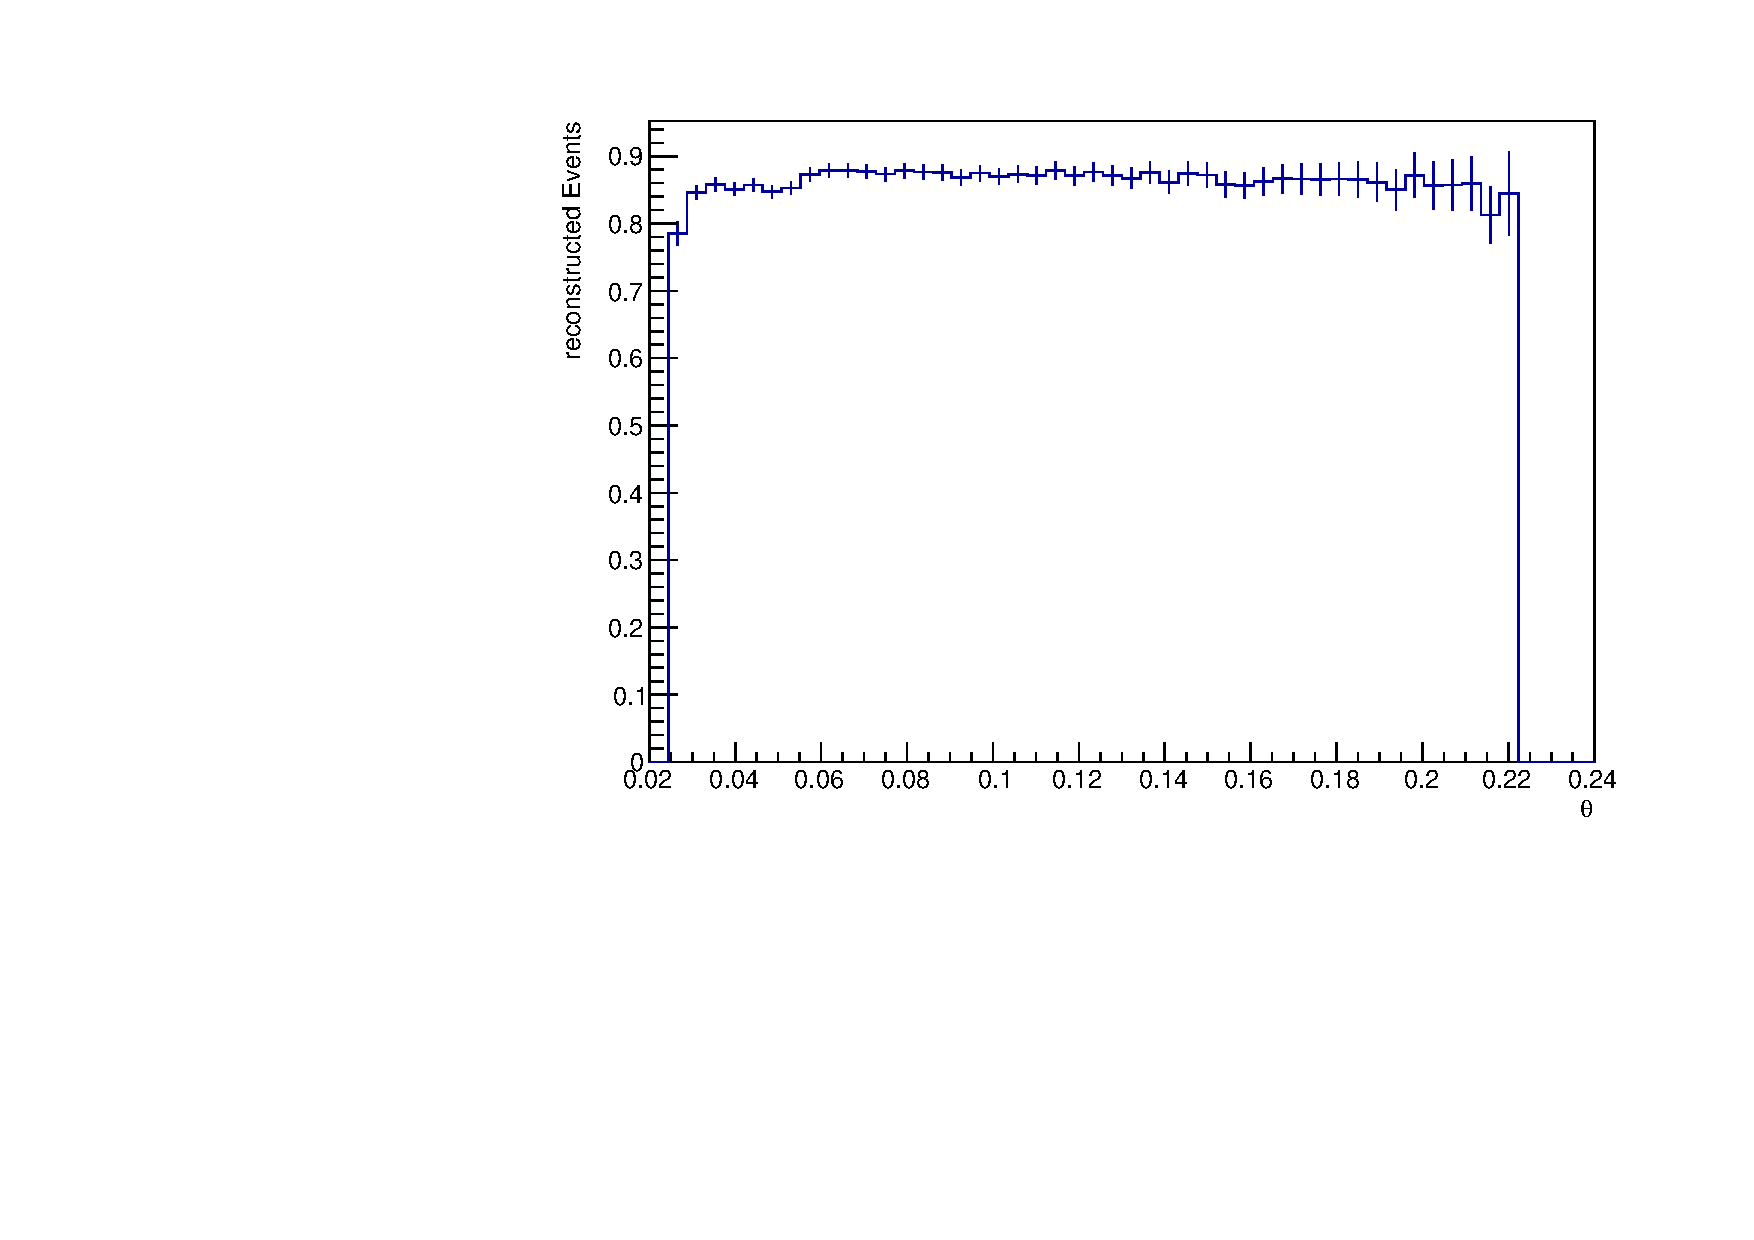
\includegraphics[width=0.9\textwidth]{up_pdf/neg/h_theta_reco_Pi_neg.pdf}
\end{subfigure}
\begin{subfigure}{0.45\textwidth}
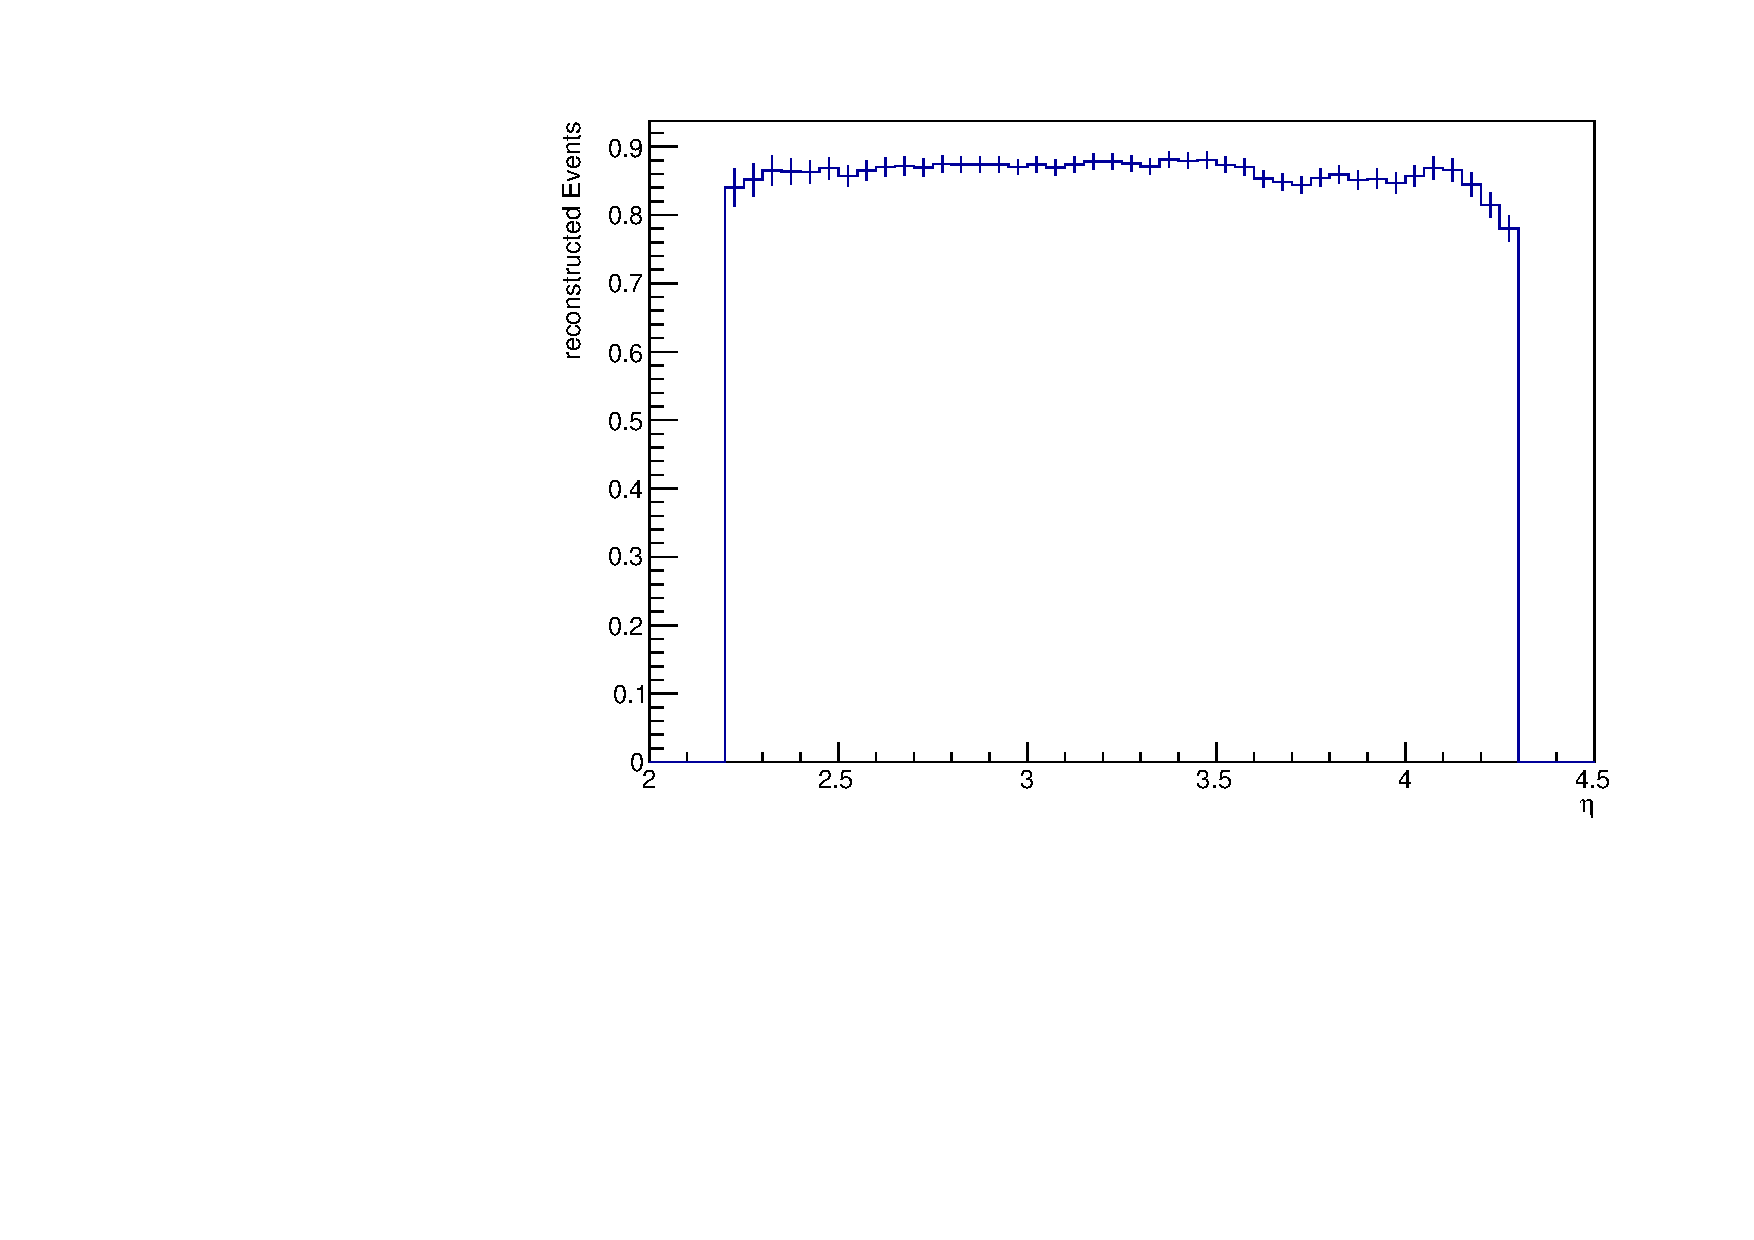
\includegraphics[width=0.9\textwidth]{up_pdf/neg/h_eta_reco_Pi_neg.pdf}
\end{subfigure}
\end{figure}
\end{frame}
\begin{frame}{$K$-efficiency}
\begin{figure}
\begin{subfigure}{0.45\textwidth}
\includegraphics[width=0.9\textwidth]{up_pdf/neg/h_pt_reco_K_neg.pdf}
\end{subfigure}
\begin{subfigure}{0.45\textwidth}
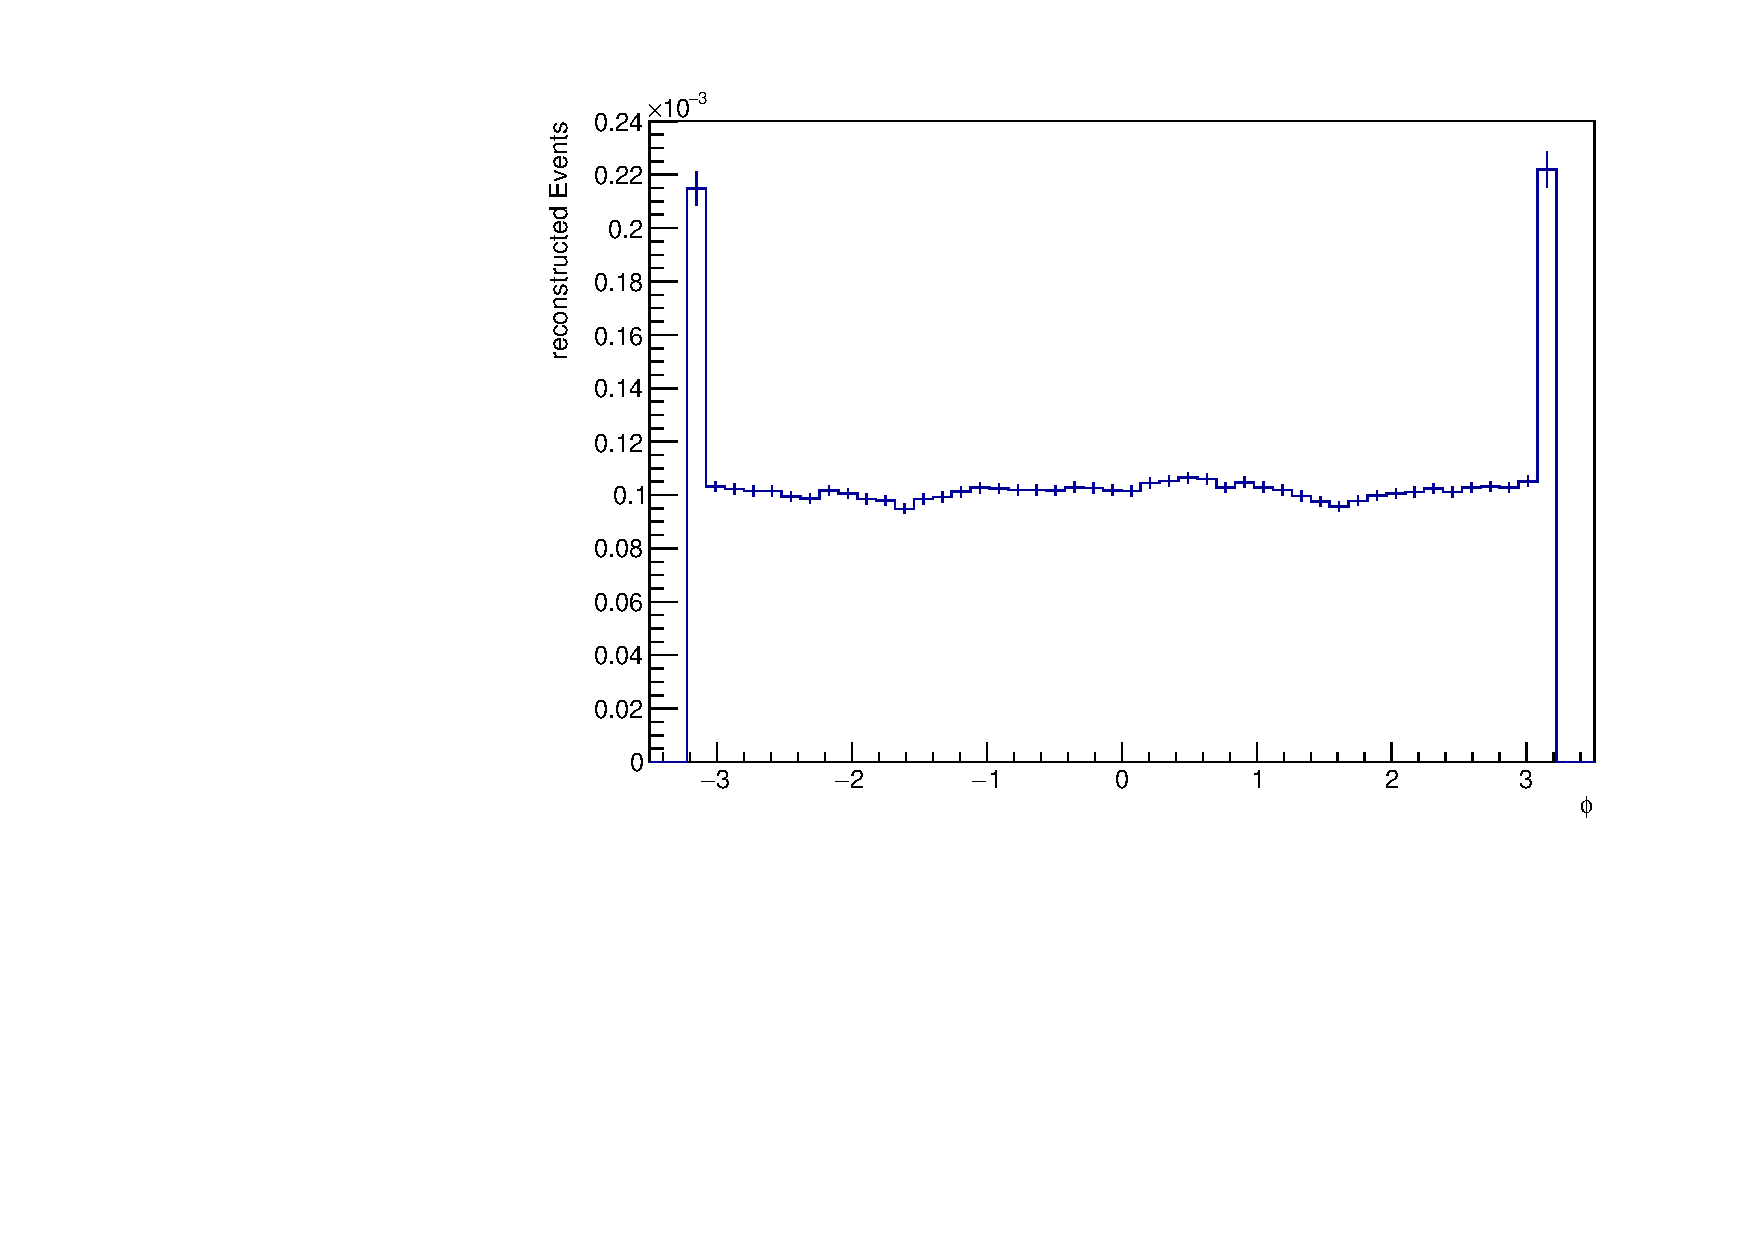
\includegraphics[width=0.9\textwidth]{up_pdf/neg/h_phi_reco_K_neg.pdf}
\end{subfigure}
\begin{subfigure}{0.45\textwidth}
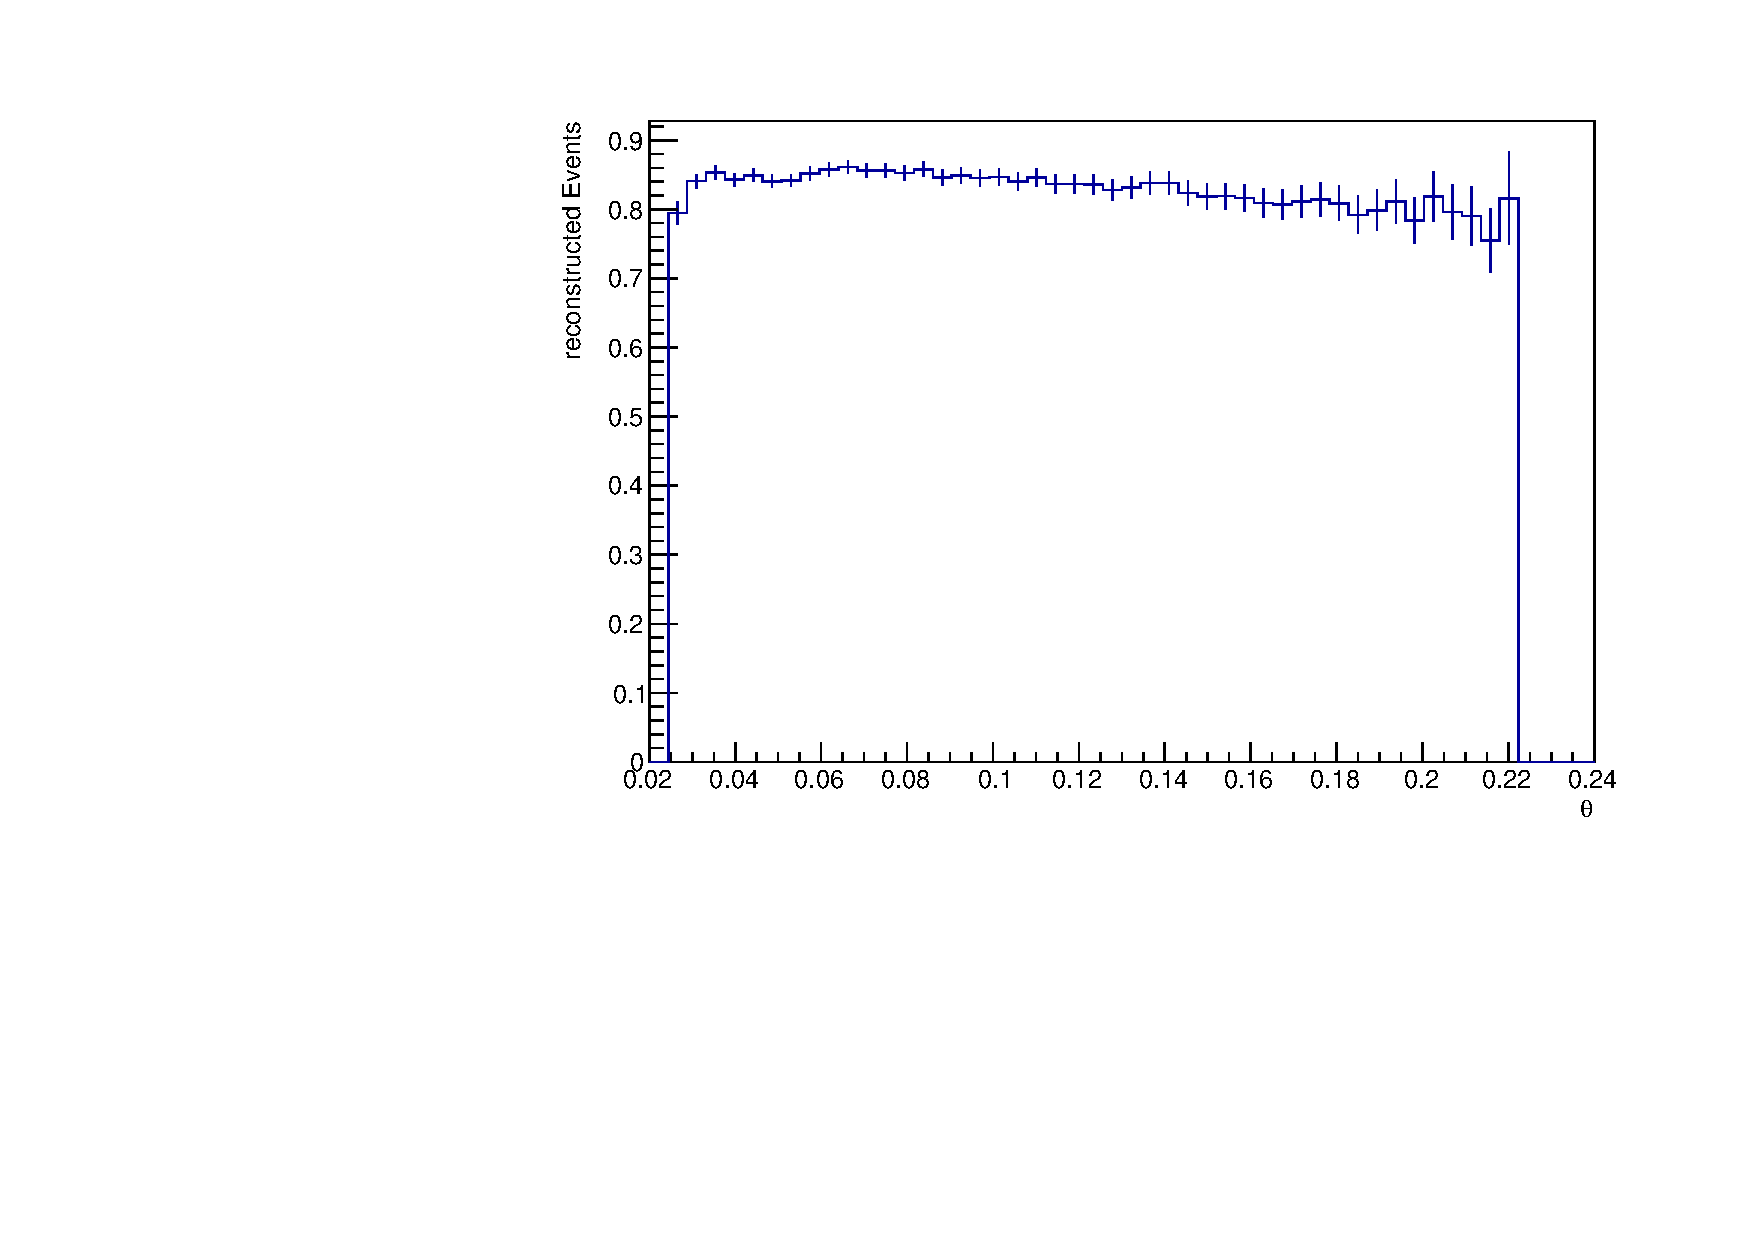
\includegraphics[width=0.9\textwidth]{up_pdf/neg/h_theta_reco_K_neg.pdf}
\end{subfigure}
\begin{subfigure}{0.45\textwidth}
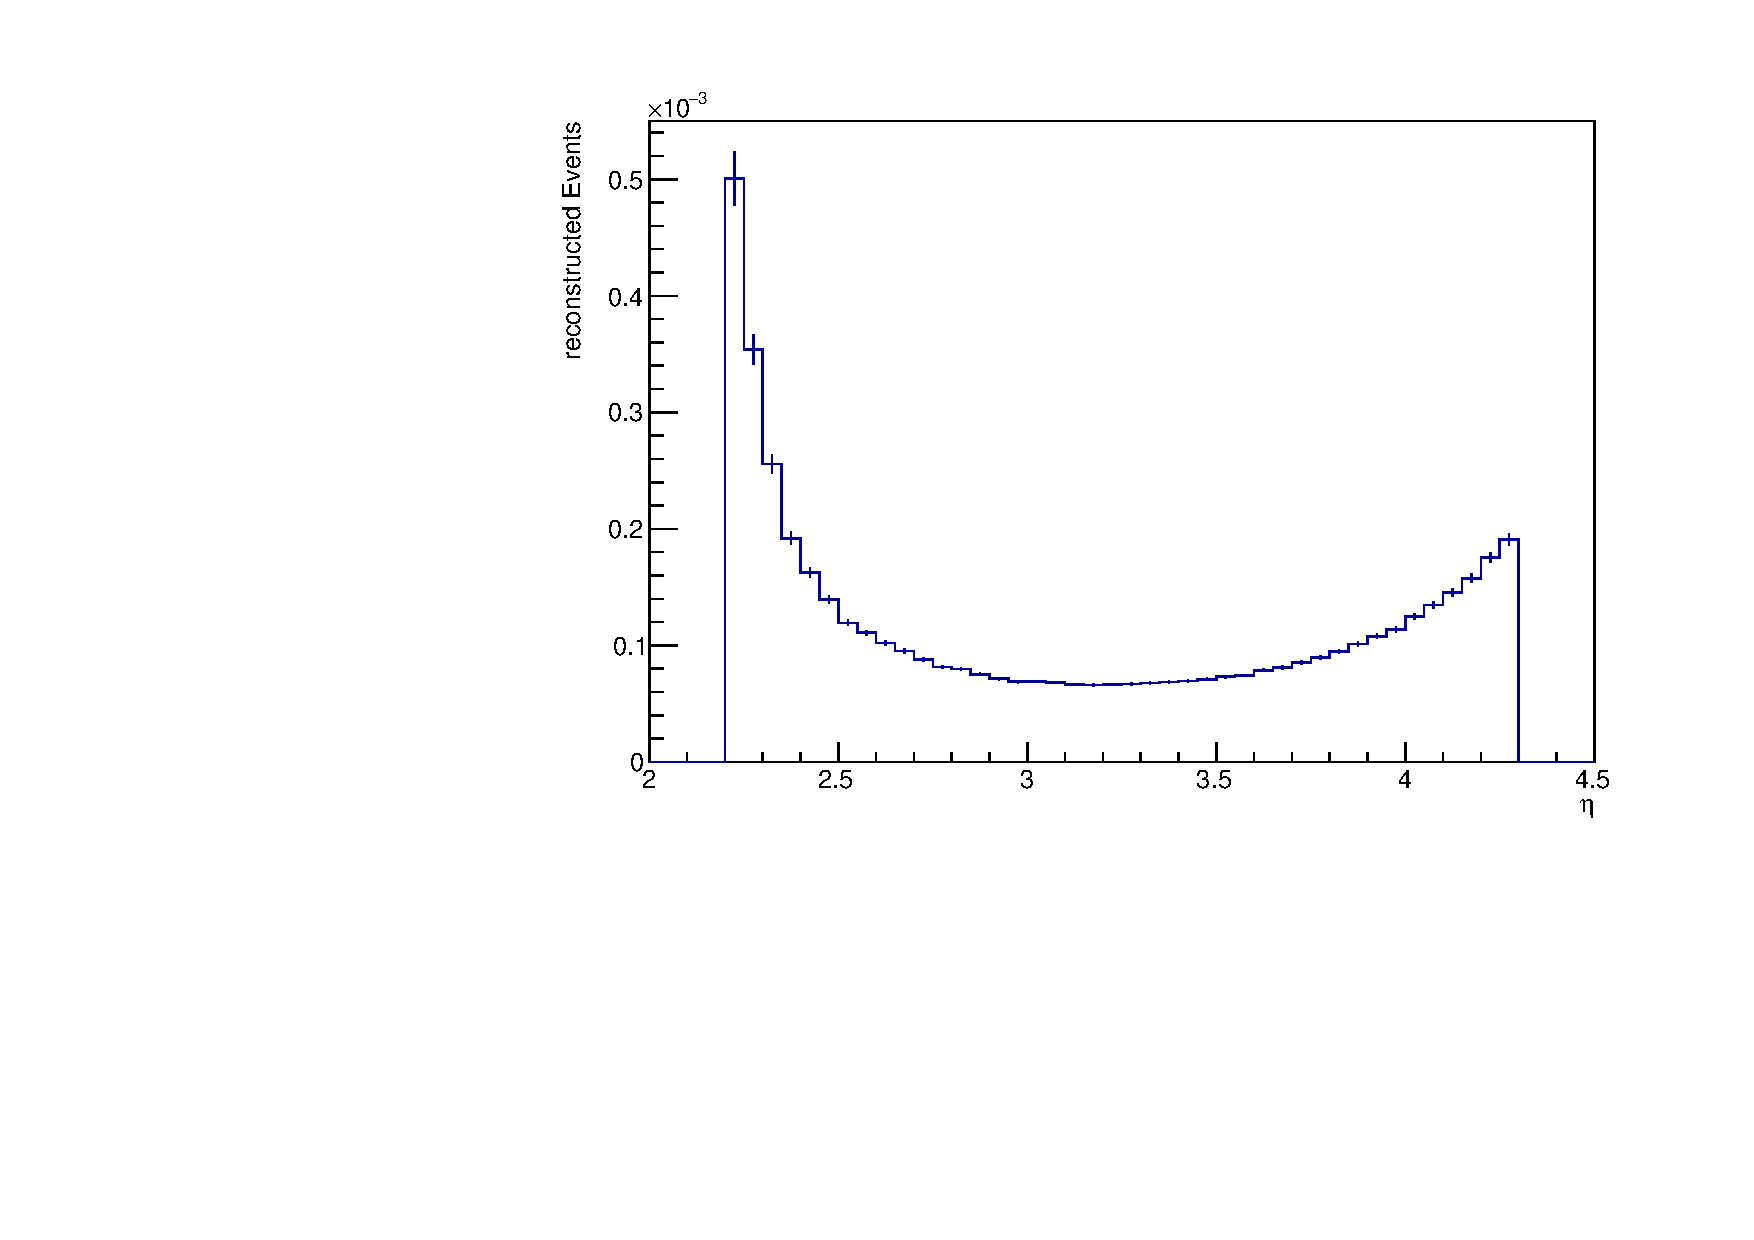
\includegraphics[width=0.9\textwidth]{up_pdf/neg/h_eta_reco_K_neg.pdf}
\end{subfigure}
\end{figure}
\end{frame}
\begin{frame}{soft $\pi$-efficiency}
\begin{figure}
\begin{subfigure}{0.45\textwidth}
\includegraphics[width=0.9\textwidth]{up_pdf/neg/h_pt_reco_SPi_neg.pdf}
\end{subfigure}
\begin{subfigure}{0.45\textwidth}
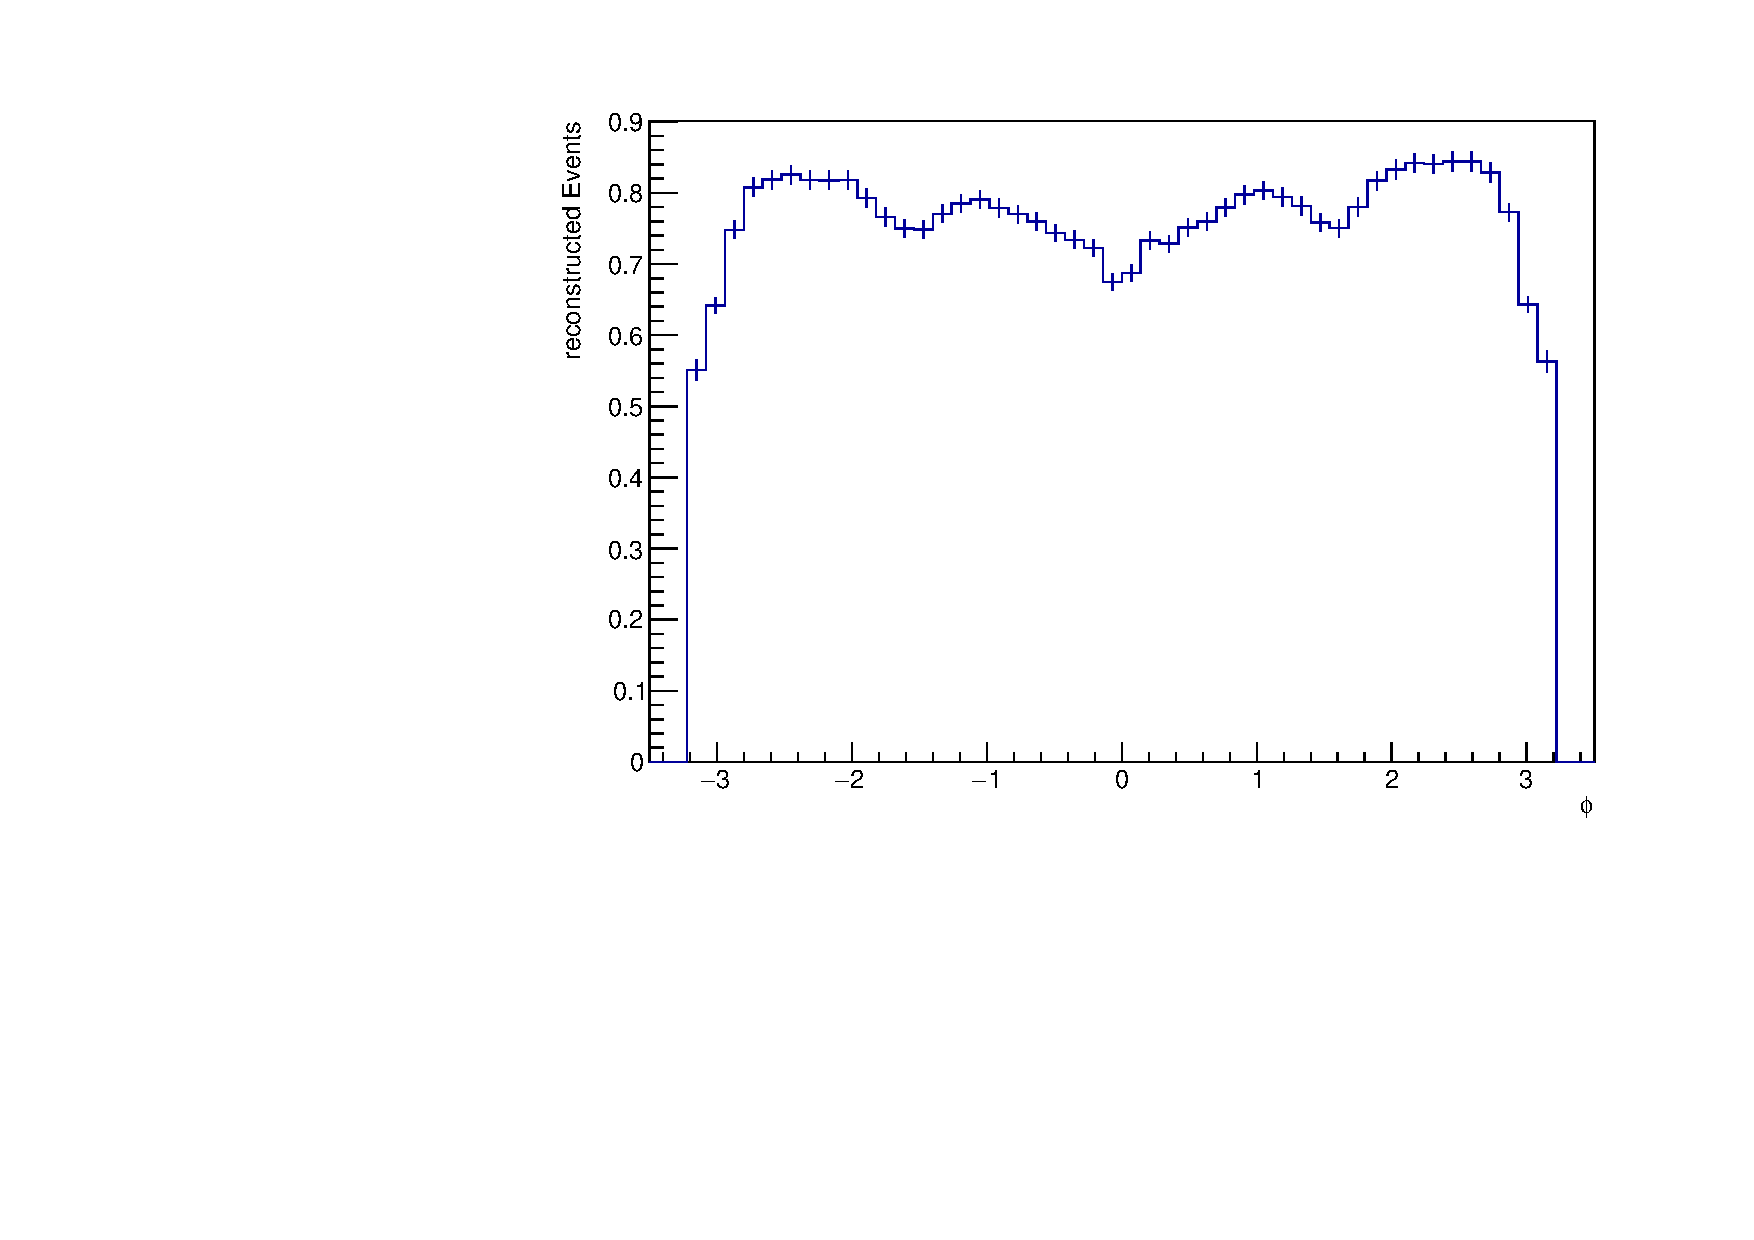
\includegraphics[width=0.9\textwidth]{up_pdf/neg/h_phi_reco_SPi_neg.pdf}
\end{subfigure}
\begin{subfigure}{0.45\textwidth}
\includegraphics[width=0.9\textwidth]{up_pdf/neg/h_theta_reco_SPi_neg.pdf}
\end{subfigure}
\begin{subfigure}{0.45\textwidth}
\includegraphics[width=0.9\textwidth]{up_pdf/neg/h_eta_reco_SPi_neg.pdf}
\end{subfigure}
\end{figure}
\end{frame}
\begin{frame}{$D^0$-efficiency}
\begin{figure}
\begin{subfigure}{0.45\textwidth}
\includegraphics[width=0.9\textwidth]{up_pdf/neg/h_pt_reco_D0_neg.pdf}
\end{subfigure}
\begin{subfigure}{0.45\textwidth}
\includegraphics[width=0.9\textwidth]{up_pdf/neg/h_phi_reco_D0_neg.pdf}
\end{subfigure}
\begin{subfigure}{0.45\textwidth}
\includegraphics[width=0.9\textwidth]{up_pdf/neg/h_theta_reco_D0_neg.pdf}
\end{subfigure}
\begin{subfigure}{0.45\textwidth}
\includegraphics[width=0.9\textwidth]{up_pdf/neg/h_eta_reco_D0_neg.pdf}
\end{subfigure}
\end{figure}
\end{frame}
\begin{frame}{$D^*$-efficiency}
\begin{figure}
\begin{subfigure}{0.45\textwidth}
\includegraphics[width=0.9\textwidth]{up_pdf/neg/h_pt_reco_Dst_neg.pdf}
\end{subfigure}
\begin{subfigure}{0.45\textwidth}
\includegraphics[width=0.9\textwidth]{up_pdf/neg/h_phi_reco_Dst_neg.pdf}
\end{subfigure}
\begin{subfigure}{0.45\textwidth}
\includegraphics[width=0.9\textwidth]{up_pdf/neg/h_theta_reco_Dst_neg.pdf}
\end{subfigure}
\begin{subfigure}{0.45\textwidth}
\includegraphics[width=0.9\textwidth]{up_pdf/neg/h_eta_reco_Dst_neg.pdf}
\end{subfigure}
\end{figure}
\end{frame}
\end{document}
